% This file was converted to LaTeX by Writer2LaTeX ver. 1.4
% see http://writer2latex.sourceforge.net for more info
\documentclass[a4paper]{article}
\usepackage[ascii]{inputenc}
\usepackage[T1]{fontenc}
\usepackage[english,portuges]{babel}
\usepackage{amsmath}
\usepackage{amssymb,amsfonts,textcomp}
\usepackage{color}
\usepackage{array}
\usepackage{supertabular}
\usepackage{hhline}
\usepackage{hyperref}
\hypersetup{pdftex, colorlinks=true, linkcolor=blue, citecolor=blue, filecolor=blue, urlcolor=blue, pdftitle=FAESA -- FACULDADES INTEGRADAS ESP\'IRITO SANTENSE, pdfauthor=Windows User, pdfsubject=, pdfkeywords=}
\usepackage[pdftex]{graphicx}
% footnotes configuration
\makeatletter
\renewcommand\thefootnote{\arabic{footnote}}
\makeatother
% Text styles
\newcommand\textstyleTtuloChar[1]{\textsf{\textbf{#1}}}
\makeatletter
\newcommand\arraybslash{\let\\\@arraycr}
\makeatother
% List styles
\newcounter{saveenum}
\newcommand\liststyleWWviiiNumi{%
\renewcommand\theenumi{\arabic{enumi}}
\renewcommand\theenumii{\arabic{enumi}.\arabic{enumii}}
\renewcommand\theenumiii{\arabic{enumi}.\arabic{enumii}.\arabic{enumiii}}
\renewcommand\theenumiv{\arabic{enumi}.\arabic{enumii}.\arabic{enumiii}.\arabic{enumiv}}
\renewcommand\labelenumi{\theenumi}
\renewcommand\labelenumii{\theenumii}
\renewcommand\labelenumiii{\theenumiii}
\renewcommand\labelenumiv{\theenumiv.}
}
\newcommand\liststyleWWviiiNumxxvii{%
\renewcommand\theenumi{\alph{enumi}}
\renewcommand\theenumii{\alph{enumii}}
\renewcommand\theenumiii{\roman{enumiii}}
\renewcommand\theenumiv{\arabic{enumiv}}
\renewcommand\labelenumi{\theenumi)}
\renewcommand\labelenumii{\theenumii.}
\renewcommand\labelenumiii{\theenumiii.}
\renewcommand\labelenumiv{\theenumiv.}
}
\newcommand\liststyleWWviiiNumiii{%
\renewcommand\theenumi{\alph{enumi}}
\renewcommand\theenumii{\arabic{enumii}}
\renewcommand\theenumiii{\arabic{enumiii}}
\renewcommand\theenumiv{\arabic{enumiv}}
\renewcommand\labelenumi{\theenumi)}
\renewcommand\labelenumii{\theenumii.}
\renewcommand\labelenumiii{\theenumiii.}
\renewcommand\labelenumiv{\theenumiv.}
}
\newcommand\liststyleWWviiiNumxviii{%
\renewcommand\theenumi{\alph{enumi}}
\renewcommand\theenumii{\alph{enumii}}
\renewcommand\theenumiii{\roman{enumiii}}
\renewcommand\theenumiv{\arabic{enumiv}}
\renewcommand\labelenumi{\theenumi)}
\renewcommand\labelenumii{\theenumii.}
\renewcommand\labelenumiii{\theenumiii.}
\renewcommand\labelenumiv{\theenumiv.}
}
\newcommand\liststyleWWviiiNumxii{%
\renewcommand\theenumi{\alph{enumi}}
\renewcommand\theenumii{\arabic{enumii}}
\renewcommand\theenumiii{\arabic{enumiii}}
\renewcommand\theenumiv{\arabic{enumiv}}
\renewcommand\labelenumi{\theenumi)}
\renewcommand\labelenumii{\theenumii.}
\renewcommand\labelenumiii{\theenumiii.}
\renewcommand\labelenumiv{\theenumiv.}
}
\newcommand\liststyleWWviiiNumxxv{%
\renewcommand\theenumi{\alph{enumi}}
\renewcommand\theenumii{\alph{enumii}}
\renewcommand\theenumiii{\roman{enumiii}}
\renewcommand\theenumiv{\arabic{enumiv}}
\renewcommand\labelenumi{\theenumi)}
\renewcommand\labelenumii{\theenumii.}
\renewcommand\labelenumiii{\theenumiii.}
\renewcommand\labelenumiv{\theenumiv.}
}
\newcommand\liststyleWWviiiNumxxxvi{%
\renewcommand\theenumi{\alph{enumi}}
\renewcommand\theenumii{\alph{enumii}}
\renewcommand\theenumiii{\roman{enumiii}}
\renewcommand\theenumiv{\arabic{enumiv}}
\renewcommand\labelenumi{\theenumi)}
\renewcommand\labelenumii{\theenumii.}
\renewcommand\labelenumiii{\theenumiii.}
\renewcommand\labelenumiv{\theenumiv.}
}
\newcommand\liststyleWWviiiNumxi{%
\renewcommand\theenumi{\alph{enumi}}
\renewcommand\theenumii{\alph{enumii}}
\renewcommand\theenumiii{\roman{enumiii}}
\renewcommand\theenumiv{\arabic{enumiv}}
\renewcommand\labelenumi{\theenumi)}
\renewcommand\labelenumii{\theenumii.}
\renewcommand\labelenumiii{\theenumiii.}
\renewcommand\labelenumiv{\theenumiv.}
}
\newcommand\liststyleWWviiiNumxxvi{%
\renewcommand\theenumi{\alph{enumi}}
\renewcommand\theenumii{\alph{enumii}}
\renewcommand\theenumiii{\roman{enumiii}}
\renewcommand\theenumiv{\arabic{enumiv}}
\renewcommand\labelenumi{\theenumi)}
\renewcommand\labelenumii{\theenumii.}
\renewcommand\labelenumiii{\theenumiii.}
\renewcommand\labelenumiv{\theenumiv.}
}
\newcommand\liststyleWWviiiNumxxviii{%
\renewcommand\theenumi{\alph{enumi}}
\renewcommand\theenumii{\alph{enumii}}
\renewcommand\theenumiii{\roman{enumiii}}
\renewcommand\theenumiv{\arabic{enumiv}}
\renewcommand\labelenumi{\theenumi)}
\renewcommand\labelenumii{\theenumii.}
\renewcommand\labelenumiii{\theenumiii.}
\renewcommand\labelenumiv{\theenumiv.}
}
\newcommand\liststyleWWviiiNumix{%
\renewcommand\theenumi{\alph{enumi}}
\renewcommand\theenumii{\alph{enumii}}
\renewcommand\theenumiii{\roman{enumiii}}
\renewcommand\theenumiv{\arabic{enumiv}}
\renewcommand\labelenumi{\theenumi)}
\renewcommand\labelenumii{\theenumii.}
\renewcommand\labelenumiii{\theenumiii.}
\renewcommand\labelenumiv{\theenumiv.}
}
\newcommand\liststyleWWviiiNumxxxviii{%
\renewcommand\theenumi{\alph{enumi}}
\renewcommand\theenumii{\alph{enumii}}
\renewcommand\theenumiii{\roman{enumiii}}
\renewcommand\theenumiv{\arabic{enumiv}}
\renewcommand\labelenumi{\theenumi)}
\renewcommand\labelenumii{\theenumii.}
\renewcommand\labelenumiii{\theenumiii.}
\renewcommand\labelenumiv{\theenumiv.}
}
\newcommand\liststyleWWviiiNumxv{%
\renewcommand\theenumi{\alph{enumi}}
\renewcommand\theenumii{\alph{enumii}}
\renewcommand\theenumiii{\roman{enumiii}}
\renewcommand\theenumiv{\arabic{enumiv}}
\renewcommand\labelenumi{\theenumi)}
\renewcommand\labelenumii{\theenumii.}
\renewcommand\labelenumiii{\theenumiii.}
\renewcommand\labelenumiv{\theenumiv.}
}
\newcommand\liststyleWWviiiNumviii{%
\renewcommand\theenumi{\alph{enumi}}
\renewcommand\theenumii{\alph{enumii}}
\renewcommand\theenumiii{\roman{enumiii}}
\renewcommand\theenumiv{\arabic{enumiv}}
\renewcommand\labelenumi{\theenumi)}
\renewcommand\labelenumii{\theenumii.}
\renewcommand\labelenumiii{\theenumiii.}
\renewcommand\labelenumiv{\theenumiv.}
}
\newcommand\liststyleWWviiiNumxvii{%
\renewcommand\theenumi{\alph{enumi}}
\renewcommand\theenumii{\alph{enumii}}
\renewcommand\theenumiii{\roman{enumiii}}
\renewcommand\theenumiv{\arabic{enumiv}}
\renewcommand\labelenumi{\theenumi)}
\renewcommand\labelenumii{\theenumii.}
\renewcommand\labelenumiii{\theenumiii.}
\renewcommand\labelenumiv{\theenumiv.}
}
\newcommand\liststyleWWviiiNumxiv{%
\renewcommand\theenumi{\alph{enumi}}
\renewcommand\theenumii{\alph{enumii}}
\renewcommand\theenumiii{\roman{enumiii}}
\renewcommand\theenumiv{\arabic{enumiv}}
\renewcommand\labelenumi{\theenumi)}
\renewcommand\labelenumii{\theenumii.}
\renewcommand\labelenumiii{\theenumiii.}
\renewcommand\labelenumiv{\theenumiv.}
}
\newcommand\liststyleWWviiiNumxxx{%
\renewcommand\theenumi{\alph{enumi}}
\renewcommand\theenumii{\alph{enumii}}
\renewcommand\theenumiii{\roman{enumiii}}
\renewcommand\theenumiv{\arabic{enumiv}}
\renewcommand\labelenumi{\theenumi)}
\renewcommand\labelenumii{\theenumii.}
\renewcommand\labelenumiii{\theenumiii.}
\renewcommand\labelenumiv{\theenumiv.}
}
\newcommand\liststyleWWviiiNumxxi{%
\renewcommand\theenumi{\alph{enumi}}
\renewcommand\theenumii{\alph{enumii}}
\renewcommand\theenumiii{\roman{enumiii}}
\renewcommand\theenumiv{\arabic{enumiv}}
\renewcommand\labelenumi{\theenumi)}
\renewcommand\labelenumii{\theenumii.}
\renewcommand\labelenumiii{\theenumiii.}
\renewcommand\labelenumiv{\theenumiv.}
}
\newcommand\liststyleWWviiiNumxiii{%
\renewcommand\theenumi{\alph{enumi}}
\renewcommand\theenumii{\alph{enumii}}
\renewcommand\theenumiii{\roman{enumiii}}
\renewcommand\theenumiv{\arabic{enumiv}}
\renewcommand\labelenumi{\theenumi)}
\renewcommand\labelenumii{\theenumii.}
\renewcommand\labelenumiii{\theenumiii.}
\renewcommand\labelenumiv{\theenumiv.}
}
\newcommand\liststyleWWviiiNumx{%
\renewcommand\theenumi{\alph{enumi}}
\renewcommand\theenumii{\alph{enumii}}
\renewcommand\theenumiii{\roman{enumiii}}
\renewcommand\theenumiv{\arabic{enumiv}}
\renewcommand\labelenumi{\theenumi)}
\renewcommand\labelenumii{\theenumii.}
\renewcommand\labelenumiii{\theenumiii.}
\renewcommand\labelenumiv{\theenumiv.}
}
\newcommand\liststyleWWviiiNumxix{%
\renewcommand\theenumi{\alph{enumi}}
\renewcommand\theenumii{\alph{enumii}}
\renewcommand\theenumiii{\roman{enumiii}}
\renewcommand\theenumiv{\arabic{enumiv}}
\renewcommand\labelenumi{\theenumi)}
\renewcommand\labelenumii{\theenumii.}
\renewcommand\labelenumiii{\theenumiii.}
\renewcommand\labelenumiv{\theenumiv.}
}
\newcommand\liststyleWWviiiNumxx{%
\renewcommand\theenumi{\alph{enumi}}
\renewcommand\theenumii{\alph{enumii}}
\renewcommand\theenumiii{\roman{enumiii}}
\renewcommand\theenumiv{\arabic{enumiv}}
\renewcommand\labelenumi{\theenumi)}
\renewcommand\labelenumii{\theenumii.}
\renewcommand\labelenumiii{\theenumiii.}
\renewcommand\labelenumiv{\theenumiv.}
}
\newcommand\liststyleWWviiiNumxxxii{%
\renewcommand\theenumi{\alph{enumi}}
\renewcommand\theenumii{\alph{enumii}}
\renewcommand\theenumiii{\roman{enumiii}}
\renewcommand\theenumiv{\arabic{enumiv}}
\renewcommand\labelenumi{\theenumi)}
\renewcommand\labelenumii{\theenumii.}
\renewcommand\labelenumiii{\theenumiii.}
\renewcommand\labelenumiv{\theenumiv.}
}
\newcommand\liststyleWWviiiNumxxxvii{%
\renewcommand\theenumi{\alph{enumi}}
\renewcommand\theenumii{\alph{enumii}}
\renewcommand\theenumiii{\roman{enumiii}}
\renewcommand\theenumiv{\arabic{enumiv}}
\renewcommand\labelenumi{\theenumi)}
\renewcommand\labelenumii{\theenumii.}
\renewcommand\labelenumiii{\theenumiii.}
\renewcommand\labelenumiv{\theenumiv.}
}
\newcommand\liststyleWWviiiNumxxxv{%
\renewcommand\theenumi{\alph{enumi}}
\renewcommand\theenumii{\alph{enumii}}
\renewcommand\theenumiii{\roman{enumiii}}
\renewcommand\theenumiv{\arabic{enumiv}}
\renewcommand\labelenumi{\theenumi)}
\renewcommand\labelenumii{\theenumii.}
\renewcommand\labelenumiii{\theenumiii.}
\renewcommand\labelenumiv{\theenumiv.}
}
% Page layout (geometry)
\setlength\voffset{-1in}
\setlength\hoffset{-1in}
\setlength\topmargin{3cm}
\setlength\oddsidemargin{3cm}
\setlength\textheight{19.977001cm}
\setlength\textwidth{16.001cm}
\setlength\footskip{1.3610001cm}
\setlength\headheight{1.73cm}
\setlength\headsep{1.632cm}
% Footnote rule
\setlength{\skip\footins}{0.119cm}
\renewcommand\footnoterule{\vspace*{-0.018cm}\setlength\leftskip{0pt}\setlength\rightskip{0pt plus 1fil}\noindent\textcolor{black}{\rule{0.25\columnwidth}{0.018cm}}\vspace*{0.101cm}}
% Pages styles
\makeatletter
\newcommand\ps@Standard{
  \renewcommand\@oddhead{}
  \renewcommand\@evenhead{}
  \renewcommand\@oddfoot{}
  \renewcommand\@evenfoot{}
  \renewcommand\thepage{\arabic{page}}
}
\newcommand\ps@Convertii{
  \renewcommand\@oddhead{\thepage{}}
  \renewcommand\@evenhead{\@oddhead}
  \renewcommand\@oddfoot{}
  \renewcommand\@evenfoot{\@oddfoot}
  \renewcommand\thepage{\arabic{page}}
}
\newcommand\ps@Converti{
  \renewcommand\@oddhead{}
  \renewcommand\@evenhead{\@oddhead}
  \renewcommand\@oddfoot{}
  \renewcommand\@evenfoot{\@oddfoot}
  \renewcommand\thepage{\arabic{page}}
}
\makeatother
\pagestyle{Standard}
\setlength\tabcolsep{1mm}
\renewcommand\arraystretch{1.3}
\title{FAESA -- FACULDADES INTEGRADAS ESP\'IRITO SANTENSE}
\author{Windows User}
\date{2012-12-19}
\begin{document}
\clearpage\setcounter{page}{1}\pagestyle{Standard}
{\centering\selectlanguage{portuges}\sffamily\bfseries
FUNDA\c{C}\~AO DE ASSIST\^ENCIA E EDUCA\c{C}\~AO - FAESA
\par}

{\centering\selectlanguage{portuges}\sffamily\bfseries
FACULDADES INTEGRADAS ESP\'IRITO-SANTENSE
\par}

{\centering\selectlanguage{portuges}\sffamily\bfseries
CURSO DE GRADUA\c{C}\~AO EM SISTEMAS DE INFORMA\c{C}\~AO
\par}


\bigskip


\bigskip


\bigskip


\bigskip


\bigskip


\bigskip


\bigskip


\bigskip


\bigskip

{\centering\selectlanguage{portuges}\sffamily\bfseries
EDGAR ELER
\par}


\bigskip


\bigskip


\bigskip


\bigskip


\bigskip


\bigskip


\bigskip


\bigskip


\bigskip


\bigskip


\bigskip

{\centering\selectlanguage{portuges}
\textsf{\textbf{A INTELIG\^ENCIA DE NEG\'OCIOS COMO FERRAMENTA M\'OVEL DE GEST\~AO DE VENDAS NUMA EMPRESA DE COM\'ERCIO
DE FERRAGENS}}
\par}


\bigskip


\bigskip


\bigskip


\bigskip


\bigskip


\bigskip


\bigskip


\bigskip


\bigskip


\bigskip


\bigskip


\bigskip


\bigskip


\bigskip


\bigskip


\bigskip


\bigskip


\bigskip


\bigskip


\bigskip

{\centering\selectlanguage{portuges}\sffamily
VIT\'ORIA
\par}

{\centering\selectlanguage{portuges}
\textsf{2012}
\par}

{\centering\selectlanguage{portuges}\sffamily\bfseries
EDGAR ELER
\par}


\bigskip


\bigskip


\bigskip


\bigskip


\bigskip


\bigskip


\bigskip


\bigskip


\bigskip


\bigskip


\bigskip


\bigskip


\bigskip


\bigskip


\bigskip


\bigskip


\bigskip

{\centering\selectlanguage{portuges}
\textsf{\textbf{A INTELIG\^ENCIA DE NEG\'OCIOS COMO FERRAMENTA M\'OVEL DE GEST\~AO DE VENDAS NUMA EMPRESA DE COM\'ERCIO
DE FERRAGENS}}
\par}


\bigskip


\bigskip


\bigskip


\bigskip


\bigskip


\bigskip


\bigskip


\bigskip


\bigskip


\bigskip

{\selectlanguage{portuges}
\textsf{Trabalho de Conclus\~ao do Curso de Gradua\c{c}\~ao em Sistemas de Informa\c{c}\~ao apresentado \`as Faculdades
Integradas Esp\'irito-Santenses como requisito parcial para a obten\c{c}\~ao do t\'itulo de Bacharel em Sistemas de
Informa\c{c}\~ao, sob orienta\c{c}\~ao da prof{\textordfeminine}. Denise Franzotti Togneri.}}


\bigskip


\bigskip


\bigskip


\bigskip


\bigskip


\bigskip


\bigskip


\bigskip


\bigskip

{\centering\selectlanguage{portuges}\sffamily
VIT\'ORIA
\par}

{\centering\selectlanguage{portuges}
\textsf{2012}
\par}

\clearpage\setcounter{page}{1}\pagestyle{Converti}
{\centering\selectlanguage{portuges}\sffamily\bfseries
[Warning: Draw object ignored]EDGAR ELER
\par}


\bigskip


\bigskip


\bigskip


\bigskip


\bigskip


\bigskip


\bigskip


\bigskip


\bigskip


\bigskip


\bigskip


\bigskip


\bigskip


\bigskip


\bigskip


\bigskip

{\centering\selectlanguage{portuges}\sffamily\bfseries
A INTELIG\^ENCIA DE NEG\'OCIOS COMO FERRAMENTA DE
\par}

{\centering\selectlanguage{portuges}\sffamily\bfseries
GEST\~AO DE VENDAS NUMA EMPRESA DE COM\'ERCIO DE
\par}

{\centering\selectlanguage{portuges}\sffamily\bfseries
FERRAGENS
\par}


\bigskip


\bigskip


\bigskip


\bigskip


\bigskip


\bigskip


\bigskip

{\selectlanguage{portuges}\sffamily\bfseries
BANCA EXAMINADORA}


\bigskip


\bigskip

{\selectlanguage{portuges}\sffamily\bfseries
\_\_\_\_\_\_\_\_\_\_\_\_\_\_\_\_\_\_\_\_\_\_\_\_\_\_\_\_\_\_\_\_}

{\selectlanguage{portuges}\sffamily
Denise Franzotti Togneri}

{\selectlanguage{portuges}\sffamily
Orientadora}


\bigskip


\bigskip

{\selectlanguage{portuges}\sffamily\bfseries
\_\_\_\_\_\_\_\_\_\_\_\_\_\_\_\_\_\_\_\_\_\_\_\_\_\_\_\_\_\_\_\_}

{\selectlanguage{portuges}\sffamily
Eliana Caus Sampaio}


\bigskip


\bigskip

{\selectlanguage{portuges}\sffamily\bfseries
\_\_\_\_\_\_\_\_\_\_\_\_\_\_\_\_\_\_\_\_\_\_\_\_\_\_\_\_\_\_\_\_}

{\selectlanguage{portuges}\sffamily
Tiago Wirtti}


\bigskip


\bigskip


\bigskip


\bigskip


\bigskip


\bigskip

{\selectlanguage{portuges}
\foreignlanguage{portuges}{\textsf{\textbf{VIT\'ORIA, 10 DE DEZEMBRO DE 2012.}}}}


\bigskip


\bigskip


\bigskip


\bigskip


\bigskip


\bigskip


\bigskip


\bigskip


\bigskip


\bigskip


\bigskip


\bigskip


\bigskip


\bigskip


\bigskip


\bigskip


\bigskip


\bigskip


\bigskip


\bigskip


\bigskip


\bigskip


\bigskip


\bigskip


\bigskip


\bigskip


\bigskip


\bigskip


\bigskip


\bigskip


\bigskip


\bigskip

{\selectlanguage{portuges}
\textsf{\textit{A melhor maneira de prever o futuro \'e invent\'a-lo.}}}

{\raggedleft\selectlanguage{portuges}
\textsf{\textit{\ \ \ \ \ \ \ \ \ \ \ \ \ \ \ \ \ \ \ \ \ \ \ \ \ \ \ \ \ \ \ \ \ \ \ \ \ \ \ \ Alan Curtis Kay}}
\par}

\clearpage{\centering\selectlanguage{portuges}\sffamily\bfseries
AGRADECIMENTOS
\par}


\bigskip

\foreignlanguage{portuges}{\textsf{Reconhe\c{c}o e gostaria de agradecer a todos aqueles que diretamente ou
indiretamente me auxiliaram na realiza\c{c}\~ao deste trabalho de conclus\~ao de curso.}}

{\selectlanguage{portuges}
\textsf{Em primeiro momento, a Deus. Ele me manteve firme, fornecendo sustento, energia emocional e espiritual, me
direcionando ao objetivo final do trabalho e ao t\'ermino de mais uma etapa de minha vida.}}

{\selectlanguage{portuges}
\textsf{\`A minha fam\'ilia, pela profunda capacidade de entender a minha \'ardua caminhada, e por sempre acreditar no
meu sucesso e, em muitos momentos, o amor e o apoio deles era a certeza que precisava para prosseguir.}}

{\selectlanguage{portuges}
\textsf{\`A orientadora, Professora Denise Franzotti Togneri, pois esta foi de fundamental import\^ancia para o
desenvolvimento desta monografia. Os conhecimentos adquiridos somente demonstram o enorme esfor\c{c}o, a confian\c{c}a
depositada, disponibilidade e dedica\c{c}\~ao que a mesma teve ao longo das orienta\c{c}\~oes.}}

{\selectlanguage{portuges}
\textsf{Aos meus amigos, que compartilharam momentos de perto ou de longe, felizes ou tristes, minha eterna
gratid\~ao.}}

{\selectlanguage{portuges}
\textsf{Aos professores, que contribu\'iram para a minha forma\c{c}\~ao acad\^emica, passando todo conhecimento
poss\'ivel.}}

{\selectlanguage{portuges}
\textsf{Aos funcion\'arios e \`a FAESA, pois foi nesse \^ambito em que convivi e aprendi a refletir em torno da vida
profissional e suas in\'umeras possibilidades, al\'em de que souberam estruturar o curso, mantendo a ordem e diretriz
acad\^emica.}}

{\selectlanguage{portuges}
\textsf{Finalmente, meus mais sinceros agradecimentos a todos pela oportunidade e credibilidade. Deus aben\c{c}oe a
voc\^es.}\textsf{\textbf{ }}}

\clearpage{\centering\selectlanguage{portuges}\sffamily\bfseries
RESUMO
\par}


\bigskip

{\selectlanguage{portuges}
[Warning: Draw object ignored]\textsf{A gest\~ao de vendas de uma empresa de com\'ercio de ferragens \'e um desafio que
envolve principalmente muito planejamento e tomada correta de decis\~oes. Para a tomada destas decis\~oes \'e
fundamental o conhecimento da realidade da empresa. N\~ao \'e poss\'ivel se conhecer a realidade correta da empresa,
mais especificamente das vendas da empresa, caso o gestor n\~ao disponha de ferramentas que lhe forne\c{c}am
informa\c{c}\~oes capazes de se montar uma vis\~ao clara sobre o desempenho da empresa e como proceder mediante estas
informa\c{c}\~oes. Outra necessidade que eles possuem \'e de que estas informa\c{c}\~oes possam ser acessadas de
qualquer lugar onde estejam, uma vez que a mobilidade dos gestores de vendas da empresa \'e alta. Para a gera\c{c}\~ao
destas informa\c{c}\~oes, prop\~oe-se a cria\c{c}\~ao de um Sistema de Informa\c{c}\~oes Gerenciais (SIG) M\'ovel para
a gest\~ao de vendas. Este sistema disp\~oe de relat\'orios e gr\'aficos espec\'ificos que atendem \`a demanda
apresentada pela gest\~ao de vendas, que podem ser acessados por meio de Tablets com os sistemas operacionais Android,
da Google, ou iOS, da Apple. Os requisitos a serem atendidos foram levantados junto ao gerente de vendas da empresa de
ferragens e modelados utilizando-se Diagrama de Casos de Uso. As informa\c{c}\~oes foram modeladas adotando-se o modelo
floco de neve e o prot\'otipo do sistema foi constru\'ido usando-se as ferramentas MicroStrategy, Pentaho Data
Integration, Oracle Database 11g, Windows Server 2008 e o Android 4.0. A partir destes relat\'orios, o gestor de vendas
ir\'a dispor de informa\c{c}\~oes valiosas e que o apoiar\~ao na correta tomada de decis\~ao para a \'area de vendas,
foco do neg\'ocio de uma empresa de com\'ercio de ferragens.}\foreignlanguage{portuges}{\textsf{ }}}


\bigskip

{\selectlanguage{portuges}\sffamily
Palavras-chave: Intelig\^encia de Neg\'ocios; Sistemas de Informa\c{c}\~oes Gerenciais; Gest\~ao de Vendas; Com\'ercio
de Ferragens.}

\clearpage{\centering\selectlanguage{english}\sffamily\bfseries
ABSTRACT
\par}


\bigskip

{\selectlanguage{portuges}
\foreignlanguage{english}{\textsf{The sales management of a hardware store company is a challenge that mainly involves a
lot of planning and make the right decisions. For make these right decisions is crucial to understand the reality of
the company. It is not possible to know the correct reality of the company, more specifically the reality of the sales
of the company, if the manager doesn't have tools that provide information able to assemble a clearly vision about the
performance of the company and how to proceed through this information. Another company's demand is that they need to
access these information anywhere, because the mobility of the company's sales managers is high. To generate this
information, is proposed the creation of a Mobile Management Information System (MIS) to the sales management. This
system has specific reports and charts that fit with the demand made by the sales management that can be accessed by
Tablets with the operational systems Android, from Google, and the iOS, from Apple. The requirements to be filled were
obtained with the company's sales manager and were designed using the Use-Case Diagram. The information were designed
adopting the snow-flake model and the prototype of the system was built using the tools MicroStrategy, Pentaho Data
Integration, Oracle Database 11g, Windows Server 2008 and the Android 4.0 From these reports, the sales manager will
have value information that will support him to make the right decision to the sales area, the business focus of a
hardware store company. }}}


\bigskip

{\selectlanguage{portuges}
\foreignlanguage{english}{\textsf{Keywords: Business Intelligence; Management Information Systems; Sales Management;
Hardware Sales.}}}

\clearpage{\centering\selectlanguage{portuges}\sffamily\bfseries
LISTA DE FIGURAS
\par}


\bigskip

{\selectlanguage{portuges}\sffamily\itshape
\textup{Figura 1: Como os SIG adquirem seus dados do SPT da empresa\ \ 24}}

{\selectlanguage{portuges}\sffamily\itshape
\textup{Figura 2: Componentes do SIG\ \ 25}}

{\selectlanguage{portuges}\sffamily\itshape
\textup{Figura 3: Exemplo de um modelo relacional ou tradicional\ \ 31}}

{\selectlanguage{portuges}\sffamily\itshape
\textup{Figura 4: Exemplo de um modelo dimensional\ \ 32}}

{\selectlanguage{portuges}\sffamily\itshape
\textup{Figura 5: Um exemplo de dados baseados em assuntos/neg\'ocios\ \ 33}}

{\selectlanguage{portuges}\sffamily\itshape
\textup{Figura 6: A quest\~ao da integra\c{c}\~ao\ \ 34}}

{\selectlanguage{portuges}\sffamily\itshape
\textup{Figura 7: A quest\~ao da n\~ao-volatidade\ \ 34}}

{\selectlanguage{portuges}\sffamily\itshape
\textup{Figura 8: A quest\~ao da varia\c{c}\~ao em rela\c{c}\~ao ao tempo\ \ 35}}

{\selectlanguage{portuges}\sffamily\itshape
\textup{Figura 9: Cubo tri-dimensional de dados de venda que possui as dimens\~oes Loja (Store), Tempo (Time) e Produto
(Product), e o fato de valores medidos (measure values)\ \ 36}}

{\selectlanguage{portuges}\sffamily\itshape
\textup{Figura 10: Modelagem estrela para um banco de dados de vendas, mostrando o relacionamento das chaves
prim\'arias\ \ 44}}

{\selectlanguage{portuges}\sffamily\itshape
\textup{Figura 11: Uma modelagem floco de neve\ \ 45}}

{\selectlanguage{portuges}\sffamily\itshape
\textup{Figura 12: Arquitetura t\'ipica de um sistema de BI\ \ 47}}

{\selectlanguage{portuges}\sffamily\itshape
\textup{Figura 13: Organograma da NIB Ferragens\ \ 49}}

{\selectlanguage{portuges}\sffamily\itshape
\textup{Figura 14: Diagrama de casos de uso principal proposto para a gest\~ao de vendas da NIB\ \ 52}}

{\selectlanguage{portuges}\sffamily\itshape
\textup{Figura 15: Diagrama de casos de uso GerenciarVendas\ \ 53}}

{\selectlanguage{portuges}\sffamily\itshape
\textup{Figura 16: Diagrama de casos de uso DemonstrarMetas\ \ 55}}

{\selectlanguage{portuges}\sffamily\itshape
\textup{Figura 17: Modelo Dimensional de Dados\ \ 61}}

{\selectlanguage{portuges}\sffamily\itshape
\textup{Figura 18: Fluxo de execu\c{c}\~ao do sistema\ \ 68}}

{\selectlanguage{portuges}\sffamily\itshape
\textup{Figura 19: Arquitetura do Sistema\ \ 71}}

{\selectlanguage{portuges}\sffamily\itshape
\textup{Figura 20: Tela inicial do sistema\ \ 73}}

{\selectlanguage{portuges}\sffamily\itshape
\textup{Figura 21: Tela do Hist\'orico de Vendas\ \ 74}}

{\selectlanguage{portuges}\sffamily\itshape
\textup{Figura 22: Tela de Produtos\ \ 75}}

{\selectlanguage{portuges}\sffamily\itshape
\textup{Figura 23: Tela de Regi\~oes\ \ 76}}


\bigskip


\bigskip

\clearpage{\centering\selectlanguage{portuges}\sffamily\bfseries
LISTA DE QUADROS
\par}


\bigskip

{\selectlanguage{portuges}\sffamily\itshape
\textup{Quadro 1: As Caracter\'isticas da Informa\c{c}\~ao Valiosa\ \ 19}}

{\selectlanguage{portuges}\sffamily\itshape
\textup{Quadro 2: Compara\c{c}\~ao entre os SADs e os SIGs\ \ 28}}

{\selectlanguage{portuges}\sffamily\itshape
\textup{Quadro 3: Compara\c{c}\~ao entre modelo relacional e modelo dimensional\ \ 31}}


\bigskip

\clearpage{\centering
\foreignlanguage{portuges}{\textsf{\textbf{LISTA DE ABREVIATURAS E SIGLAS}}}
\par}


\bigskip

\foreignlanguage{portuges}{\textsf{BI -- Business Intelligence}}

\foreignlanguage{english}{\textsf{CRM -- Customer Relationship Management}}

{\selectlanguage{english}\sffamily
DM -- Data Mart}

{\selectlanguage{english}\sffamily
DW -- Data Warehouse}

\foreignlanguage{english}{\textsf{DOLAP -- Dimensional Online Analytical Processing}}

\foreignlanguage{english}{\textsf{ERM -- Enterprise Relationship Management}}

\foreignlanguage{english}{\textsf{ERP -- Enterprise Resource Planning}}

\foreignlanguage{english}{\textsf{ETL -- Extract Transform Load}}

\foreignlanguage{english}{\textsf{HOLAP -- Hybrid Online Analytical Processing}}

\foreignlanguage{english}{\textsf{MOLAP -- Multidimensional Online Analytical Processing}}

{\selectlanguage{english}\sffamily
ODS -- Operational Data Store}

\foreignlanguage{english}{\textsf{OLAP -- Online Analytical Processing}}

\foreignlanguage{portuges}{\textsf{OLTP \ {}- Online Transaction Processing}}

\foreignlanguage{portuges}{\textsf{SGBD -- Sistema de Gerenciamento de Banco de Dados}}

\foreignlanguage{english}{\textsf{ROLAP -- Relational Online Transaction Processing}}

{\selectlanguage{portuges}\sffamily
SAD -- Sistema de Apoio \`a Decis\~ao}

{\selectlanguage{portuges}
\textsf{SIG -- Sistema de Informa\c{c}\~oes Gerenciais}}

\clearpage\setcounter{page}{1}\pagestyle{Convertii}
{\centering\selectlanguage{portuges}\sffamily\bfseries
SUM\'ARIO
\par}


\bigskip

{\sffamily\bfseries
\textstyleTtuloChar{1 introdu\c{c}\~ao\textmd{\ \ }\foreignlanguage{portuges}{\textmd{14}}}}

{\selectlanguage{portuges}\sffamily\scshape
1.1 O PROBLEMA\ \ 15}

{\selectlanguage{portuges}\sffamily\scshape
1.2 HIP\'OTESE\ \ 15}

{\selectlanguage{portuges}\sffamily\scshape
1.3 OBJETIVOS\ \ 15}

{\selectlanguage{portuges}\sffamily\itshape
\textbf{\textup{1.3.1 Geral}}\textup{\ \ 15}}

{\selectlanguage{portuges}\sffamily\itshape
\textbf{\textup{1.3.2 Espec\'ificos}}\textup{\ \ 15}}

{\selectlanguage{portuges}\sffamily\itshape
\textup{1.4 JUSTIFICATIVA\ \ 16}}

{\selectlanguage{portuges}\sffamily\scshape
1.5 METODOLOGIA\ \ 16}

{\selectlanguage{portuges}\sffamily\scshape
1.6 ORGANIZA\c{C}\~AO DA MONOGRAFIA\ \ 16}

{\sffamily\bfseries
\textstyleTtuloChar{2 Sistemas de Informa\c{c}\~oes Gerenciais\textmd{\ \ }\foreignlanguage{portuges}{\textmd{18}}}}

{\selectlanguage{portuges}\sffamily\scshape
2.1 A INFORMA\c{C}\~AO NO PROCESSO DECIS\'ORIO\ \ 18}

{\selectlanguage{portuges}\sffamily\scshape
2.2 MANIPULA\c{C}\~AO E ESTRUTURA\c{C}\~AO DA INFORMA\c{C}\~AO\ \ 20}

{\selectlanguage{portuges}\sffamily\scshape
2.3 SISTEMAS DE INFORMA\c{C}\~OES GERENCIAIS (SIG), SISTEMAS DE APOIO \`A DECIS\~AO (SAD) E INTELIG\^ENCIA DE NEG\'OCIOS
(BUSINESS INTELLIGENCE - BI)\ \ 22}

{\selectlanguage{portuges}\sffamily\itshape
\textbf{\textup{2.3.1 Sistemas de Informa\c{c}\~oes Gerenciais (SIG)}}\textup{\ \ 23}}

{\selectlanguage{portuges}\sffamily\itshape
\textbf{\textup{2.3.2 Sistemas de Apoio \`a Decis\~ao (SAD)}}\textup{\ \ 27}}

{\selectlanguage{portuges}\sffamily\itshape
\textbf{\textup{2.3.3 Diferen\c{c}as entre SIG e SAD}}\textup{\ \ 27}}

{\selectlanguage{portuges}\sffamily\itshape
\textbf{\textup{2.3.4 Business Intelligence (BI)}}\textup{\ \ 29}}

{\selectlanguage{portuges}\sffamily\scshape
2.4 MODELAGEM DE UM SISTEMA DE BI\ \ 36}

{\selectlanguage{portuges}\sffamily\itshape
\textbf{\textup{2.4.1 Etapas para constru\c{c}\~ao de um Sistema de BI}}\textup{\ \ 36}}

{\selectlanguage{portuges}\sffamily\itshape
\textbf{\textup{2.4.2 Armazenamento de Dados}}\textup{\ \ 41}}

{\selectlanguage{portuges}\sffamily\scshape
2.5 FERRAMENTAS E TECNOLOGIAS PARA A MONTAGEM DOS RELAT\'ORIOS\ \ 46}

{\sffamily\bfseries
\textstyleTtuloChar{3 ESTUDO DE CASO: NIB FERRAGENS\textmd{\ \ }\foreignlanguage{portuges}{\textmd{48}}}}

{\selectlanguage{portuges}\sffamily\scshape
3.1 NIB FERRAGENS\ \ 48}

{\selectlanguage{portuges}\sffamily\scshape
3.2 REQUISITOS FUNCIONAIS PARA APOIO \`A GEST\~AO DE VENDAS\ \ 51}

{\selectlanguage{portuges}\sffamily\itshape
\textbf{\textup{3.2.1 Caso de uso GerenciarVendas}}\textup{\ \ 52}}

{\selectlanguage{portuges}\sffamily\itshape
\textbf{\textup{3.2.2 Caso de uso DemonstrarMetas}}\textup{\ \ 55}}

{\selectlanguage{portuges}\sffamily\scshape
3.3 PROPOSTA DE UM SIG DE VENDAS\ \ 56}

{\selectlanguage{portuges}\sffamily\scshape
3.4 TRABALHOS CORRELATOS\ \ 58}

{\selectlanguage{portuges}\sffamily\scshape
\textstyleTtuloChar{4 AN\'ALISE E PROJETO\textmd{\ \ 60}}}

{\selectlanguage{portuges}\sffamily\scshape
4.1 AN\'ALISE E MODELAGEM DIMENSIONAL DOS DADOS\ \ 60}

{\selectlanguage{portuges}\sffamily\scshape
4.2 TECNOLOGIAS UTILIZADAS NA PROTOTIPA\c{C}\~AO\ \ 64}

{\selectlanguage{portuges}\sffamily\itshape
\textbf{\textup{4.2.1 Armazenamento do Data Mart}}\textup{\ \ 64}}

{\selectlanguage{portuges}\sffamily\itshape
\textbf{\textup{4.2.2 Camada de ETL}}\textup{\ \ 65}}

{\selectlanguage{portuges}\sffamily\itshape
\textbf{\textup{4.2.3 Mapeamento do Modelo Dimensional e da Camada Visual}}\textup{\ \ 65}}

{\selectlanguage{portuges}\sffamily\itshape
\textbf{\textup{4.2.4 Camada de Servidor}}\textup{\ \ 66}}

{\selectlanguage{portuges}\sffamily\itshape
\textbf{\textup{4.2.5 Plataforma M\'ovel -- Camada de Acesso \`as Informa\c{c}\~oes}}\textup{\ \ 67}}

{\selectlanguage{portuges}\sffamily\scshape
4.3 RESTRI\c{C}\~OES DE IMPLEMENTA\c{C}\~AO\ \ 67}

{\selectlanguage{portuges}\sffamily\scshape
4.4 FLUXO DE EXECU\c{C}\~AO\ \ 68}

{\selectlanguage{portuges}\sffamily\scshape
4.5 ARQUITETURA DO SISTEMA\ \ 70}

{\selectlanguage{portuges}\sffamily\scshape
4.6 PROT\'OTIPO DO SISTEMA\ \ 72}

{\sffamily\bfseries
\textstyleTtuloChar{5 CONCLUS\~OES E PERSPECTIVAS FUTURAS\textmd{\ \ }\foreignlanguage{portuges}{\textmd{77}}}}

{\sffamily\bfseries
\textstyleTtuloChar{6 REFER\^ENCIAS\textmd{\ \ 7}\foreignlanguage{portuges}{\textmd{9}}}}


\bigskip


\bigskip


\bigskip

\liststyleWWviiiNumi
\begin{enumerate}
\item \clearpage{\selectlanguage{portuges}\sffamily\bfseries
INTRODU\c{C}\~AO}
\end{enumerate}

\bigskip

{\selectlanguage{portuges}\sffamily
A NIB Ferragens Ltda., uma organiza\c{c}\~ao com 30 anos de hist\'oria, \'e uma empresa do ramo de com\'ercio de
ferragens para constru\c{c}\~ao civil, com matriz na cidade de Cariacica -- ES.}

{\selectlanguage{portuges}
\textsf{A empresa hoje possui diversos Sistemas de Processamento de Transa\c{c}\~ao}\footnote{\ \textsf{Sistemas de
Processamento de Transa\c{c}\~ao ``s\~ao os que tratam das transa\c{c}\~oes rotineiras, repetitivas e comuns da
organiza\c{c}\~ao, pertinentes ao curso normal dos neg\'ocios, trabalhando com dados detalhados sobre essas
transa\c{c}\~oes'' (Beal, 2004, p. 18).}\par \par }\textsf{ (SPT), tais como sistema financeiro, de gerenciamento de
produtos, de vendas, de faturamento e de log\'istica. A organiza\c{c}\~ao possui diversas filiais que utilizam estoques
e pre\c{c}os diferentes, dependendo de cada localidade, n\~ao possuindo, para um controle e gerenciamento de vendas,
sistemas que auxiliem os processos decis\'orios relacionados \`a \'area de vendas.}}

{\selectlanguage{portuges}
\textsf{Os gestores de vendas da NIB Ferragens desempenham atividades que demandam deslocamentos di\'arios, tanto para
clientes quanto entre as filiais, e atualmente os gestores apenas tem acesso aos SPTs quando est\~ao dentro da empresa,
o que gera atrasos nas tomadas de decis\~oes, algo que n\~ao ocorreria caso os gestores dispusessem de ferramentas que
fornecessem informa\c{c}\~oes numa plataforma m\'ovel.}}

{\selectlanguage{portuges}
\textsf{Para apoiar a gest\~ao de vendas, a organiza\c{c}\~ao necessita implantar neste processo um modelo que venha a
suprir a necessidade da unifica\c{c}\~ao e associa\c{c}\~ao dos dados como a rela\c{c}\~ao vendas/hora dos vendedores,
os pre\c{c}os aplicados pelos concorrentes, os pre\c{c}os aplicados pelos fornecedores, o n\'ivel de demanda do mercado
de constru\c{c}\~ao civil de determinada localidade da filial, o n\'ivel de conhecimento que o mercado de ferragens
para constru\c{c}\~ao civil da localidade da filial tem para com o nome e os produtos da empresa, obtido por meio de
pesquisa de mercado, e o custo do investimento a ser feito em marketing. A partir destas informa\c{c}\~oes coletadas,
\'e necess\'ario fornecer os relat\'orios referentes aos investimentos e mudan\c{c}as que, se forem realizados em um
tempo determinado, }\textsf{acarretar\~ao numa determinada varia\c{c}\~ao positiva no faturamento e conhecimento do
nome, da marca e dos produtos da empresa.}}


\bigskip

\liststyleWWviiiNumi
\setcounter{saveenum}{\value{enumi}}
\begin{enumerate}
\setcounter{enumi}{\value{saveenum}}
\item \setcounter{saveenum}{\value{enumii}}
\begin{enumerate}
\setcounter{enumii}{\value{saveenum}}
\item {\selectlanguage{portuges}\sffamily
O PROBLEMA}
\end{enumerate}
\end{enumerate}
{\selectlanguage{portuges}\sffamily
Como apoiar a gest\~ao m\'ovel de vendas de uma empresa de com\'ercio de ferragens que depende somente das
informa\c{c}\~oes geradas pelos diversos SPT{\textasciiacute}s implantados na empresa?}


\bigskip

\liststyleWWviiiNumi
\setcounter{saveenum}{\value{enumi}}
\begin{enumerate}
\setcounter{enumi}{\value{saveenum}}
\item \setcounter{saveenum}{\value{enumii}}
\begin{enumerate}
\setcounter{enumii}{\value{saveenum}}
\item {\selectlanguage{portuges}\sffamily
HIP\'OTESE}
\end{enumerate}
\end{enumerate}
{\selectlanguage{portuges}
\textsf{Diante dos problemas levantados, uma prov\'avel solu\c{c}\~ao \'e desenvolver um Sistema M\'ovel de
Informa\c{c}\~oes Gerenciais para a gest\~ao completa e precisa das vendas da empresa.}}


\bigskip

\liststyleWWviiiNumi
\setcounter{saveenum}{\value{enumi}}
\begin{enumerate}
\setcounter{enumi}{\value{saveenum}}
\item \setcounter{saveenum}{\value{enumii}}
\begin{enumerate}
\setcounter{enumii}{\value{saveenum}}
\item {\selectlanguage{portuges}\sffamily
OBJETIVOS}

\setcounter{saveenum}{\value{enumiii}}
\begin{enumerate}
\setcounter{enumiii}{\value{saveenum}}
\item {\selectlanguage{portuges}\sffamily\bfseries
Geral}
\end{enumerate}
\end{enumerate}
\end{enumerate}
{\selectlanguage{portuges}
\textsf{Construir um sistema m\'ovel capaz de coletar e avaliar as informa\c{c}\~oes ligadas \`as vendas da empresa.}}


\bigskip

\liststyleWWviiiNumi
\setcounter{saveenum}{\value{enumi}}
\begin{enumerate}
\setcounter{enumi}{\value{saveenum}}
\item \setcounter{saveenum}{\value{enumii}}
\begin{enumerate}
\setcounter{enumii}{\value{saveenum}}
\item \setcounter{saveenum}{\value{enumiii}}
\begin{enumerate}
\setcounter{enumiii}{\value{saveenum}}
\item {\selectlanguage{portuges}\sffamily\bfseries
Espec\'ificos}
\end{enumerate}
\end{enumerate}
\end{enumerate}
{\selectlanguage{portuges}\sffamily
Os objetivos espec\'ificos s\~ao:}

\liststyleWWviiiNumxxvii
\begin{enumerate}
\item {\selectlanguage{portuges}\sffamily
Investigar os Sistemas de Informa\c{c}\~oes Gerenciais e suas aplicabilidades na \'area de vendas;}
\item {\selectlanguage{portuges}\sffamily
Investigar a computa\c{c}\~ao m\'ovel;}
\item {\selectlanguage{portuges}\sffamily
Levantar e documentar os requisitos que dever\~ao ser atendidos por um SIG de vendas;}
\item {\selectlanguage{portuges}
\textsf{Analisar, projetar, construir e testar um SIG m\'ovel de vendas.}}
\end{enumerate}

\bigskip

\liststyleWWviiiNumi
\begin{enumerate}
\item \begin{enumerate}
\item {\selectlanguage{portuges}\sffamily
JUSTIFICATIVA}
\end{enumerate}
\end{enumerate}
{\selectlanguage{portuges}\sffamily
Na d\'ecada de 80 surge o conceito de Intelig\^encia de Neg\'ocios, baseado na coleta e explora\c{c}\~ao de
informa\c{c}\~oes corporativas de maneira que, com estas, seja poss\'ivel desenvolver solu\c{c}\~oes e caminhos
pautados para o suporte \`a tomada de decis\~ao.}

{\selectlanguage{portuges}\sffamily
Com o surgimento deste conceito, as corpora\c{c}\~oes passaram a investir parte de seu capital nas tecnologias de
Intelig\^encia de Neg\'ocios, de forma que, a partir dos relat\'orios e t\'ecnicas fornecidas pela mesma, tivessem base
segura e estrat\'egica para a correta tomada de decis\~oes.}

{\selectlanguage{portuges}
\textsf{Sendo assim, um Sistema M\'ovel de Informa\c{c}\~oes Gerenciais, aplicado na \'area de vendas, implantando as
t\'ecnicas de Intelig\^encia de Neg\'ocios, ir\'a contribuir com a empresa, uma vez que as informa\c{c}\~oes geradas
podem ser aplicadas para avalia\c{c}\~oes dos desempenhos e an\'alises de mercado, utilizando os modelos diferenciados
de disposi\c{c}\~ao e organiza\c{c}\~ao dos dados. Com estas informa\c{c}\~oes, \'e poss\'ivel viabilizar o suporte
\`as decis\~oes referentes \`a \'area de vendas, que \'e a atividade central da empresa.}}

{\selectlanguage{portuges}\sffamily
Com a Intelig\^encia de Neg\'ocios, a ger\^encia de vendas da organiza\c{c}\~ao conseguir\'a atingir em cheio os pontos
em que se deve investir, melhorar e capacitar, tra\c{c}ando um rumo e um ponto a seguir, a partir da coleta e
avalia\c{c}\~ao das informa\c{c}\~oes das vendas.}


\bigskip

\liststyleWWviiiNumi
\setcounter{saveenum}{\value{enumi}}
\begin{enumerate}
\setcounter{enumi}{\value{saveenum}}
\item \setcounter{saveenum}{\value{enumii}}
\begin{enumerate}
\setcounter{enumii}{\value{saveenum}}
\item {\selectlanguage{portuges}\sffamily
METODOLOGIA}
\end{enumerate}
\end{enumerate}
{\selectlanguage{portuges}
\textsf{Inicialmente foi feita uma revis\~ao bibliogr\'afica sobre os assuntos abordados, foram levantados os requisitos
junto ao gerente de vendas e documentados utilizando-se os diagramas de caso de uso. A an\'alise, o projeto e a
apresenta\c{c}\~ao do prot\'otipo do sistema.}}


\bigskip

\liststyleWWviiiNumi
\setcounter{saveenum}{\value{enumi}}
\begin{enumerate}
\setcounter{enumi}{\value{saveenum}}
\item \setcounter{saveenum}{\value{enumii}}
\begin{enumerate}
\setcounter{enumii}{\value{saveenum}}
\item {\selectlanguage{portuges}\sffamily
ORGANIZA\c{C}\~AO DA MONOGRAFIA}
\end{enumerate}
\end{enumerate}
{\selectlanguage{portuges}\sffamily
Este trabalho cont\'em, al\'em desta Introdu\c{c}\~ao, mais cinco cap\'itulos. }

{\selectlanguage{portuges}
\textsf{O cap\'itulo 2 -- Sistemas de Informa\c{c}\~oes Gerenciais -- aborda os conceitos de Informa\c{c}\~ao, sua
import\^ancia na tomada de decis\~oes, Sistemas de Informa\c{c}\~oes }\textsf{Gerenciais e Sistemas de Apoio \`a
Decis\~ao, estrutura\c{c}\~ao e modelagem de Intelig\^encia de Neg\'ocios.}}

{\selectlanguage{portuges}
\textsf{O cap\'itulo 3 -- Estudo de Caso: NIB Ferragens -- apresenta a estrutura organizacional da NIB Ferragens, o
problema enfrentado na Gest\~ao de Vendas da empresa, o levantamento dos requisitos funcionais e a proposta do Sistema
de Informa\c{c}\~oes Gerenciais.}}

{\selectlanguage{portuges}
\textsf{O cap\'itulo 4 -- An\'alise e Projeto -- apresenta a modelagem e o projeto do Sistema M\'ovel de
Informa\c{c}\~oes Gerenciais proposto para a Gest\~ao de Vendas da NIB Ferragens.}}

{\selectlanguage{portuges}
\textsf{O cap\'itulo 5 -- Conclus\~oes e Perspectivas Futuras -- apresenta uma descri\c{c}\~ao geral do que foi abordado
nos cap\'itulos anteriores e faz uma descri\c{c}\~ao geral sobre as possibilidades do sistema tanto na NIB Ferragens
quanto no mercado de com\'ercio em geral.}}


\bigskip


\bigskip

\liststyleWWviiiNumi
\setcounter{saveenum}{\value{enumi}}
\begin{enumerate}
\setcounter{enumi}{\value{saveenum}}
\item \clearpage{\selectlanguage{portuges}\sffamily\bfseries
SISTEMAS DE INFORMA\c{C}\~OES GERENCIAIS}
\end{enumerate}

\bigskip

{\selectlanguage{portuges}
\textsf{Este cap\'itulo aborda os conceitos de informa\c{c}\~ao, seu papel no processo decis\'orio e os meios de se
produzir esta informa\c{c}\~ao de forma clara e coerente como esperado pela ger\^encia da organiza\c{c}\~ao a fim de,
obedecendo \`as metas e objetivos dos gerentes para determinado processo ou \'area, ser base concreta para a tomada de
decis\~oes referentes ao processo ou \'area em quest\~ao.}}


\bigskip

\liststyleWWviiiNumi
\setcounter{saveenum}{\value{enumi}}
\begin{enumerate}
\setcounter{enumi}{\value{saveenum}}
\item \setcounter{saveenum}{\value{enumii}}
\begin{enumerate}
\setcounter{enumii}{\value{saveenum}}
\item {\selectlanguage{portuges}\sffamily
A INFORMA\c{C}\~AO NO PROCESSO DECIS\'ORIO}
\end{enumerate}
\end{enumerate}
{\selectlanguage{portuges}\sffamily
A informa\c{c}\~ao \'e fundamental no apoio \`as estrat\'egias e processos de tomada de decis\~ao, bem como no controle
das opera\c{c}\~oes empresariais. Sua utiliza\c{c}\~ao representa uma interven\c{c}\~ao no processo de gest\~ao,
podendo, inclusive, provocar mudan\c{c}a organizacional, \`a medida que afeta os diversos elementos que comp\~oem um
sistema de gest\~ao. Esse recurso vital da organiza\c{c}\~ao, quando devidamente estruturado, integra as fun\c{c}\~oes
das v\'arias unidades da empresa, por meio dos diversos sistemas organizacionais (BEUREN, 1998, p. 43). }

{\selectlanguage{portuges}
\textsf{A informa\c{c}\~ao \'e uma cole\c{c}\~ao de fatos organizados de modo que adquirem um valor adicional al\'em do
valor dos pr\'oprios fatos. Os dados consistem em fatos n\~ao trabalhados, sem utilidade, sem significado (STAIR;
REYNOLDS, 2002, p. 4).}}

{\selectlanguage{portuges}
\textsf{A validade e a import\^ancia da informa\c{c}\~ao s\~ao medidas de acordo com o conhecimento proporcionado por
sua exist\^encia. Conhecimento ``representa a percep\c{c}\~ao e a compreens\~ao de um conjunto de informa\c{c}\~oes e
de como estas informa\c{c}\~oes podem ser \'uteis para uma tarefa espec\'ifica''. O quadro 1 representa, de acordo com
Stair e Reynolds (2002, p. 5), as caracter\'isticas da informa\c{c}\~ao valiosa.}}


\bigskip


\bigskip


\bigskip

\begin{flushleft}
\tablefirsthead{}
\tablehead{}
\tabletail{}
\tablelasttail{}
\begin{supertabular}{|m{3.1599998cm}|m{12.458cm}|}
\hline
{\selectlanguage{portuges}\sffamily\bfseries Caracter\'isticas} &
{\selectlanguage{portuges}\sffamily\bfseries Defini\c{c}\~oes}\\\hline
{\selectlanguage{portuges}\sffamily Precisa} &
{\selectlanguage{portuges}\sffamily A informa\c{c}\~ao precisa n\~ao cont\'em erro. Em alguns casos, a informa\c{c}\~ao
imprecisa \'e gerada porque dados imprecisos s\~ao alimentados no processo de transforma\c{c}\~ao (isso \'e comumente
chamado de entra lixo e sai lixo)}\\\hline
{\selectlanguage{portuges}\sffamily Completa} &
{\selectlanguage{portuges}\sffamily A informa\c{c}\~ao completa cont\'em todos os fatos importantes. Por exemplo, um
relat\'orio de investimento que n\~ao inclua todos os custos importantes n\~ao \'e completo.}\\\hline
{\selectlanguage{portuges}\sffamily Econ\^omica} &
{\selectlanguage{portuges}\sffamily A informa\c{c}\~ao tamb\'em deve ser relativamente econ\^omica para ser viabilizada.
Os tomadores de decis\~ao sempre precisam equilibrar o valor da informa\c{c}\~ao com o custo de produzi-la.}\\\hline
{\selectlanguage{portuges}\sffamily Flex\'ivel} &
{\selectlanguage{portuges}\sffamily A informa\c{c}\~ao flex\'ivel pode ser usada para uma variedade de prop\'ositos. Por
exemplo, a informa\c{c}\~ao sobre o estoque dispon\'ivel para uma pe\c{c}a em particular pode ser \'util para o
vendedor num fechamento de venda, para o gerente de produ\c{c}\~ao, que determina a necessidade ou n\~ao de mais
estoque, e para o executivo financeiro, que especifica o valor total que a empresa investiu em estoque.}\\\hline
{\selectlanguage{portuges}\sffamily Confi\'avel} &
{\selectlanguage{portuges}\sffamily A informa\c{c}\~ao confi\'avel pode ser dependente de algum outro fator. Em muitos
casos, a confiabilidade da informa\c{c}\~ao depende do m\'etodo de coleta dos dados. Em outros exemplos, a
confiabilidade depende da fonte da informa\c{c}\~ao. Um rumor, sem fonte conhecida, sobre a eleva\c{c}\~ao de pre\c{c}o
do petr\'oleo pode n\~ao ser confi\'avel.}\\\hline
{\selectlanguage{portuges}\sffamily Relevante} &
{\selectlanguage{portuges}\sffamily A informa\c{c}\~ao relevante \'e essencial para o tomador de decis\~ao. A queda de
pre\c{c}o da madeira pode n\~ao ser relevante para um fabricante de chip de computador.}\\\hline
{\selectlanguage{portuges}\sffamily Simples} &
{\selectlanguage{portuges}\sffamily A informa\c{c}\~ao tamb\'em deve ser simples, n\~ao excessivamente complexa.
Informa\c{c}\~ao sofisticada e detalhada pode sobrecarregar o conjunto de informa\c{c}\~oes. Quando um tomador de
decis\~ao disp\~oe de muita informa\c{c}\~ao, h\'a dificuldade em determinar qual delas \'e realmente
importante.}\\\hline
{\selectlanguage{portuges}\sffamily Pontual} &
{\selectlanguage{portuges}\sffamily Informa\c{c}\~ao pontual \'e aquela obtida quando necess\'aria. Por exemplo, as
condi\c{c}\~oes do tempo para a \'ultima semana n\~ao interferir\~ao na escolha do vestir hoje.}\\\hline
{\selectlanguage{portuges}\sffamily Verific\'avel} &
{\selectlanguage{portuges} \textsf{A informa\c{c}\~ao deve ser verific\'avel. Isso significa que voc\^e pode conferi-la
e se assegurar de que est\'a correta, talvez confrontando muitas fontes para uma mesma informa\c{c}\~ao.}}\\\hline
{\selectlanguage{portuges}\sffamily Acess\'ivel} &
{\selectlanguage{portuges}\sffamily A informa\c{c}\~ao deve ser facilmente acess\'ivel aos usu\'arios autorizados.
Obt\^e-la na forma correta e no tempo certo atender\'a, certamente, a suas necessidades.}\\\hline
{\selectlanguage{portuges}\sffamily Segura} &
{\selectlanguage{portuges}\sffamily A informa\c{c}\~ao deve ser segura para possibilitar seu acesso apenas pelos
usu\'arios autorizados.}\\\hline
\end{supertabular}
\end{flushleft}
{\selectlanguage{portuges}
\textsf{QUADRO 1: As Caracter\'isticas da Informa\c{c}\~ao Valiosa. }}

{\selectlanguage{portuges}\sffamily
Fonte: STAIR; REYNOLDS, 2001, p. 6. }

{\selectlanguage{portuges}\sffamily
{}``O processo de administra\c{c}\~ao nas empresas utiliza a informa\c{c}\~ao como apoio \`as decis\~oes, atrav\'es de
sistemas informativos que observam requisitos quanto a transmissores e receptores de informa\c{c}\~oes, canais de
transmiss\~ao, conte\'udo das informa\c{c}\~oes, periodicidade das comunica\c{c}\~oes, bem como processos de
convers\~ao das informa\c{c}\~oes em decis\~oes junto a cada um dos centros de responsabilidades -- unidades
organizacionais -- da empresa.'' (REBOU\c{C}AS, 2007, p. 32). Nota-se que a informa\c{c}\~ao para quaisquer
corpora\c{c}\~oes tem fun\c{c}\~ao vital em todo processo decis\'orio e que os sistemas gerenciais s\~ao pe\c{c}as
essenciais para a gera\c{c}\~ao destas informa\c{c}\~oes v\'alidas. }

{\selectlanguage{portuges}
\textsf{\'E de consenso geral que a informa\c{c}\~ao \'e ao mesmo tempo mat\'eria-prima e produto acabado da atividade
de sistemas. E sabe-se tamb\'em que a informa\c{c}\~ao -- adequadamente estruturada -- contribui para que a empresa se
torne mais e mais din\^amica, a ponto de afirmar-se que tanto mais din\^amica ser\'a uma empresa quanto melhores e mais
adequadas forem as informa\c{c}\~oes que os gerentes disp\~oem para as suas tomadas de decis\~ao (CASSARRO, 2001, p.
34). }}

{\selectlanguage{portuges}\sffamily
A informa\c{c}\~ao \'agil sobre os processos organizacionais, com procedimentos anal\'iticos rigorosos, para fomentar
decis\~oes, n\~ao menos \'ageis, resulta num importante potencial para o gestor tomar decis\~oes muito mais acentuadas
do que aquele que se baseia apenas na sua experi\^encia e conhecimento (BEUREN, 1998, p. 77).}

{\selectlanguage{portuges}\sffamily
A partir destes dados pode-se dizer que a informa\c{c}\~ao, quando bem elaborada e estruturada, contribui em muito para
o crescimento de toda empresa. O contr\'ario tamb\'em \'e um fato a partir do momento em que temos o quadro apresentado
na maioria das empresas de pequeno e m\'edio porte, com informa\c{c}\~oes geradas em grande parte por sistemas
diferentes e n\~ao integrados, onde n\~ao se obt\'em a resposta esperada de acordo com os objetivos e metas
organizacionais da empresa, n\~ao dando suporte a quaisquer decis\~oes que a empresa venha a tomar baseada num
prospecto dos desempenhos desenvolvidos no \'ultimo per\'iodo analisado, que seria o objetivo de todo sistema
gerencial. }


\bigskip

\liststyleWWviiiNumi
\setcounter{saveenum}{\value{enumi}}
\begin{enumerate}
\setcounter{enumi}{\value{saveenum}}
\item \setcounter{saveenum}{\value{enumii}}
\begin{enumerate}
\setcounter{enumii}{\value{saveenum}}
\item {\selectlanguage{portuges}\sffamily
MANIPULA\c{C}\~AO E ESTRUTURA\c{C}\~AO DA INFORMA\c{C}\~AO}
\end{enumerate}
\end{enumerate}
{\selectlanguage{portuges}\sffamily
Os sistemas de informa\c{c}\~ao, atrav\'es da gera\c{c}\~ao de informa\c{c}\~oes para o processo decis\'orio, contribuem
para a efic\'acia do executivo no exerc\'icio das fun\c{c}\~oes de planejamento, organiza\c{c}\~ao, dire\c{c}\~ao e
controle na gest\~ao das empresas (REBOU\c{C}AS, 2007, p. 32). }

{\selectlanguage{portuges}
\textsf{Com a correta manipula\c{c}\~ao e estrutura\c{c}\~ao da informa\c{c}\~ao, pode-se tra\c{c}ar e identificar as
metas e estrat\'egias da empresa. ``A informa\c{c}\~ao pode ser visualizada e analisada em uma dupla perspectiva. Ela
pode facilitar a identifica\c{c}\~ao de alternativas inovadoras no processo de elabora\c{c}\~ao da estrat\'egia
empresarial, ou seja, ela pode apoiar a defini\c{c}\~ao estrat\'egica de outras vari\'aveis. Por outro lado, a
informa\c{c}\~ao tamb\'em pode conFigurar-se como um componente vital que se incorpora na estrat\'egia definida.''
(BEUREN, 1998, p. 51). }}

{\selectlanguage{portuges}
\textsf{Deve-se, por\'em, ter em mente que n\~ao basta apenas a gera\c{c}\~ao da informa\c{c}\~ao por si s\'o, sendo
necess\'ario que a mesma seja encaminhada aos que possuem autonomia para analisar tais informa\c{c}\~oes e tomar as
decis\~oes baseadas nestas. Para se obter informa\c{c}\~ao precisa-se compilar, reunir fatos e n\'umeros, os quais,
devidamente preparados, possibilitam a elabora\c{c}\~ao de uma dada informa\c{c}\~ao. Todavia, por melhor que seja a
informa\c{c}\~ao, se esta n\~ao for comunicada a quem de direito, todo o trabalho ter\'a sido pura perda de tempo
(CASSARRO, 2001, p. 34). }}

{\selectlanguage{portuges}\sffamily
A ado\c{c}\~ao de sistemas, modelos e tecnologias de suporte \`a decis\~ao deve ser escolhida pela alta
administra\c{c}\~ao da empresa, pois ``[...] n\~ao adianta a empresa ter um processo administrativo adequado, se faltar
um sistema estruturado de informa\c{c}\~oes gerenciais que alimente esse processo decis\'orio, bem como o
desenvolvimento, a implementa\c{c}\~ao e a avalia\c{c}\~ao das decis\~oes e a\c{c}\~oes posteriores.'' (REBOU\c{C}AS,
2007, p. 74). }

{\selectlanguage{portuges}\sffamily
O processo decis\'orio \'e baseado apenas na experi\^encia dos executivos envolvidos e sem car\'ater cient\'ifico,
dependente de dados elaborados e analisados tecnicamente. Existem m\'etodos e t\'ecnicas mais sofisticadas; por\'em, as
decis\~oes dependem muito da confian\c{c}a e da seguran\c{c}a que se tem dessas informa\c{c}\~oes. Para estimular a
utiliza\c{c}\~ao dessas informa\c{c}\~oes, podem ser criados c\'odigos e pol\'iticas que estabele\c{c}am e regulem a
aplica\c{c}\~ao e a divulga\c{c}\~ao dos dados levantados (REBOU\c{C}AS, 2007, p. 76). }

{\selectlanguage{portuges}\sffamily
A partir disto pode-se afirmar que um sistema para o gerenciamento, estrutura\c{c}\~ao e elabora\c{c}\~ao destas
informa\c{c}\~oes \'e ferramenta fundamental para o crescimento mais \'agil das empresas no mundo atual. Pode-se dizer,
tamb\'em, que sistemas mal elaborados e que gerem informa\c{c}\~oes incorretas ou num espa\c{c}o de tempo maior tendem
a atrasar ou at\'e anular o crescimento proposto e objetivado pela alta administra\c{c}\~ao da empresa. }

{\selectlanguage{portuges}\sffamily
Como via de regra e exig\^encia para a verifica\c{c}\~ao da qualidade dos sistemas, \'e preciso saber se os sistemas a
serem escolhidos e implantados ajudam a ger\^encia s\^enior a atacar e enfrentar quest\~oes estrat\'egicas e
tend\^encias de longo prazo tanto na empresa quanto no ambiente externo. Sua principal preocupa\c{c}\~ao \'e
compatibilizar as mudan\c{c}as no ambiente externo com a capacidade da organiza\c{c}\~ao. Quais ser\~ao os n\'iveis de
emprego em cinco anos? Quais s\~ao as tend\^encias de longo prazo do custo do setor e onde nossa empresa se encaixa?
Que produtos deveremos estar fazendo dentro de cinco anos? (LAUDON, 2004, p. 40). }

{\selectlanguage{portuges}\sffamily
Os executivos das empresas devem estar cientes de que as necessidades e a import\^ancia das informa\c{c}\~oes podem
crescer de maneira exponencial em rela\c{c}\~ao ao crescimento das empresas. Naturalmente, para que ocorra essa
evolu\c{c}\~ao da necessidade das informa\c{c}\~oes nas empresas \'e preciso que elas sejam confi\'aveis, relevantes e
dispon\'iveis em tempo, para proporcionar decis\~oes corretas aos executivos. E, nesse momento, deve ser considerado o
valor efetivo da informa\c{c}\~ao, que pode ser resultante de dois itens, a saber, o impacto que a informa\c{c}\~ao
provoca nas decis\~oes dos executivos e a utilidade dessa informa\c{c}\~ao, tendo em vista o seu tempo de
utiliza\c{c}\~ao pela empresa (REBOU\c{C}AS, 2007, p. 34-35).}


\bigskip

\liststyleWWviiiNumi
\setcounter{saveenum}{\value{enumi}}
\begin{enumerate}
\setcounter{enumi}{\value{saveenum}}
\item \setcounter{saveenum}{\value{enumii}}
\begin{enumerate}
\setcounter{enumii}{\value{saveenum}}
\item {\selectlanguage{portuges}
\textsf{SISTEMAS DE INFORMA\c{C}\~OES GERENCIAIS (SIG), SISTEMAS DE APOIO \`A DECIS\~AO (SAD) E INTELIG\^ENCIA DE
NEG\'OCIOS (}\textsf{\textit{BUSINESS INTELLIGENCE}}\textsf{ - BI)}}
\end{enumerate}
\end{enumerate}
{\selectlanguage{portuges}
\textsf{Nesta se\c{c}\~ao ser\~ao abordadas duas categorias de Sistemas de Informa\c{c}\~oes, os Sistemas de
Informa\c{c}\~oes Gerenciais (SIG) e os Sistemas de Apoio \`a Decis\~ao (SAD), e ser\'a explanado o conceito de
Intelig\^encia de Neg\'ocios.}}


\bigskip


\bigskip

\liststyleWWviiiNumi
\setcounter{saveenum}{\value{enumi}}
\begin{enumerate}
\setcounter{enumi}{\value{saveenum}}
\item \setcounter{saveenum}{\value{enumii}}
\begin{enumerate}
\setcounter{enumii}{\value{saveenum}}
\item \setcounter{saveenum}{\value{enumiii}}
\begin{enumerate}
\setcounter{enumiii}{\value{saveenum}}
\item {\selectlanguage{portuges}
\textsf{\textbf{Sistemas de Informa\c{c}\~oes Gerenciais (SIG)}}}
\end{enumerate}
\end{enumerate}
\end{enumerate}
{\selectlanguage{portuges}
\textsf{Os Sistemas de Informa\c{c}\~oes Gerenciais (SIG) s\~ao aqueles que apoiam o processo de transforma\c{c}\~ao de
dados em informa\c{c}\~oes que s\~ao utilizadas na estrutura decis\'oria da empresa, bem como proporcionam a
sustenta\c{c}\~ao administrativa para otimizar os resultados esperados (REBOU\c{C}AS, 1997, p. 39).}}

{\selectlanguage{portuges}
\textsf{Um SIG prov\^e suporte aos gerentes para alcan\c{c}ar suas metas corporativas, suprindo-os com
}\textsf{\textit{feedback}}\textsf{ e informa\c{c}\~oes para entender melhor as opera\c{c}\~oes regulares da
organiza\c{c}\~ao. Possibilita a compara\c{c}\~ao de resultados para se estabelecer as metas da companhia e a
identifica\c{c}\~ao de \'areas com problemas e oportunidades de aprimoramento. A partir desta compreens\~ao e
percep\c{c}\~ao melhoradas, os gerentes s\~ao capazes de controlar, organizar e planejar com mais efici\^encia e
efic\'acia. Dessa forma, um SIG efetivo pode fornecer \`a organiza\c{c}\~ao uma vantagem competitiva e, no m\'inimo,
uma margem tempor\'aria sobre outra organiza\c{c}\~ao carente de tal tipo de sistema (STAIR; REYNOLDS, 2002,
p.282-283).}}

{\selectlanguage{portuges}
\textsf{Os dados que entram em um SIG originam-se tanto de fontes internas quanto externas. A fonte de dados interna
mais significativa para um SIG s\~ao os diversos Sistemas de Processamento de Transa\c{c}\~oes e Sistemas de
Planejamento de Recursos Empresariais, bem como suas bases de dados associadas. Outros dados internos podem ser
oriundos de \'areas funcionais espec\'ificas da empresa. Fontes de dados externas podem incluir clientes, fornecedores,
competidores e acionistas, cujos dados n\~ao s\~ao capturados diretamente pelo Sistema de Processamento de
Transa\c{c}\~oes, bem como outras fontes, como a Internet, por exemplo. Al\'em disso, muitas empresas implementam
extranets como modo de conex\~ao e canal para troca de informa\c{c}\~oes com essas entidades (STAIR; REYNOLDS, 2006, p.
373).}}

{\selectlanguage{portuges}
\textsf{\ {}``O SIG usa os dados dessas fontes e os processa em informa\c{c}\~oes mais \'uteis para os gerentes,
basicamente, na forma de relat\'orios predeterminados.'' (STAIR; REYNOLDS, 2002, p. 279). Uma vez que se obtiveram os
dados por meio da entrada, os mesmos s\~ao processados e retornados como informa\c{c}\~oes \'uteis aos gerentes no
processo decis\'orio de determinado processo. }}

{\selectlanguage{portuges}
\textsf{A Figura 1 ilustra, de acordo com Laudon e Laudon (2007, p. 48), como os SIG adquirem seus dados do SPT da
empresa para o transformarem em relat\'orios aos gerentes.}}

{\selectlanguage{portuges}
 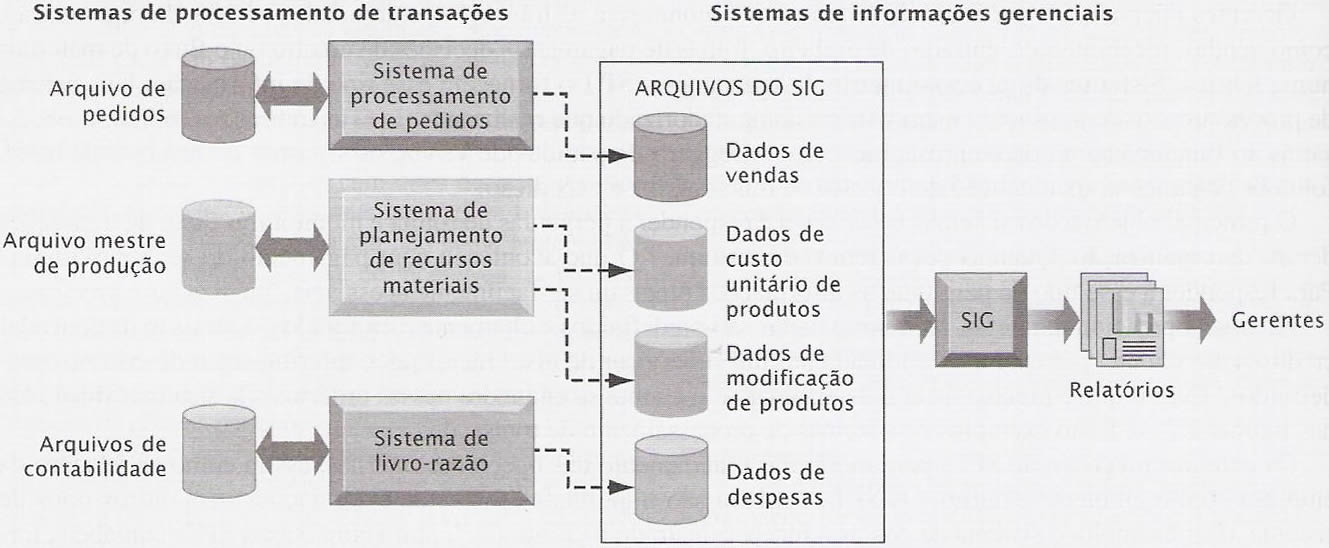
\includegraphics[width=13.115cm,height=5.413cm]{monograph-img001.jpg} \textsf{\MakeUppercase{ \newline
FIGURA }}\textsf{1: Como os SIG adquirem seus dados do SPT da empresa. }}

{\selectlanguage{portuges}\sffamily
Fonte: LAUDON; LAUDON, 2007, p. 48. }

{\selectlanguage{portuges}
\textsf{A sa\'ida da maioria dos sistemas de informa\c{c}\~oes gerenciais corresponde a um conjunto de relat\'orios que
s\~ao distribu\'idos aos gerentes. Esses relat\'orios incluem, segundo Stair e Reynolds (2002, p. 279-281) e (2006, p.
373-376):}}

\liststyleWWviiiNumiii
\begin{enumerate}
\item {\selectlanguage{portuges}
\textsf{Relat\'orios agendados. S\~ao produzidos periodicamente ou de acordo com um agendamento, di\'aria, semanal ou
mensalmente. }}
\item {\selectlanguage{portuges}
\textsf{Relat\'orios de indicadores-chave. Resumem as atividades cr\'iticas do dia anterior, estando geralmente
dispon\'iveis no in\'icio de cada jornada de trabalho. Os relat\'orios de indicadores-chave orientam gerentes e
executivos para a tomada de a\c{c}\~oes corretivas r\'apidas relacionadas a aspectos relevantes do neg\'ocio em pauta.
}}
\item {\selectlanguage{portuges}
\textsf{Relat\'orios sob demanda. Disponibilizam informa\c{c}\~oes de acordo com as exig\^encias da ger\^encia, ou
melhor, s\~ao produzidos sob demanda. }}
\item {\selectlanguage{portuges}
\textsf{Relat\'orios de exce\c{c}\~ao. S\~ao relat\'orios produzidos automaticamente quando h\'a uma situa\c{c}\~ao
incomum ou que exija uma interven\c{c}\~ao gerencial. Da mesma forma que os relat\'orios de indicadores-chave, os
relat\'orios de exce\c{c}\~ao s\~ao fundamentais para se monitorar aspectos importantes para o sucesso da
organiza\c{c}\~ao. Em geral, quando um relat\'orio de exce\c{c}\~ao \'e produzido, um gerente ou executivo deve
intervir. Os par\^ametros, ou pontos de disparo, para um relat\'orio }\textsf{de exce\c{c}\~ao devem ser cuidadosamente
conFigurados. Os pontos de disparo conFigurados muito abaixo do esperado podem resultar numa abund\^ancia de
relat\'orios de exce\c{c}\~ao; j\'a os pontos de disparo acima podem significar que problemas que exigiam uma
a\c{c}\~ao gerencial, no entanto, foram negligenciados. }}
\item {\selectlanguage{portuges}
\textsf{Relat\'orios de drill down ou relat\'orios detalhados. Fornecem resultados em n\'iveis crescentes de detalhe.
Com um relat\'orio detalhado, \'e poss\'ivel visualizar as informa\c{c}\~oes em diversos n\'iveis de detalhe --
primeiro os n\'iveis mais altos, ent\~ao n\'iveis mais detalhados e ent\~ao um n\'ivel muito detalhado. }}
\end{enumerate}
{\selectlanguage{portuges}
\textsf{Os relat\'orios gerados por sistemas de informa\c{c}\~ao gerencial podem ajudar gerentes e administradores a
elaborar melhores planos, a tomar melhores decis\~oes e a obter um maior controle sobre as opera\c{c}\~oes de suas
empresas. \'E importante notar que tipos de relat\'orios distintos podem se sobrepor. Certas recomenda\c{c}\~oes devem
ser seguidas para a elabora\c{c}\~ao e desenvolvimento de relat\'orios que sejam de algum uso (STAIR; REYNOLDS, 2006,
p. 376).}}

{\selectlanguage{portuges}
\textsf{A Figura 2 ilustra, de acordo com Rebou\c{c}as (1997, p. 140), os elementos que comp\~oem um SIG.}}

{\selectlanguage{portuges}
[Warning: Draw object ignored]\newline
\textsf{\MakeUppercase{FIGURA }}\textsf{2: Componentes do SIG. }}

{\selectlanguage{portuges}\sffamily
Fonte: REBOU\c{C}AS, 1997, p. 140. }

{\selectlanguage{portuges}\sffamily
Rebou\c{c}as (1997, p. 141-142) descreve os conceitos de cada um dos componentes do SIG da seguinte forma:}

\liststyleWWviiiNumxviii
\begin{enumerate}
\item {\selectlanguage{portuges}
\textsf{Dado \'e o elemento identificado em sua forma bruta que por si s\'o n\~ao conduz a uma compreens\~ao de um fato
ou situa\c{c}\~ao;}}
\item {\selectlanguage{portuges}
\textsf{Tratamento \'e a transforma\c{c}\~ao de um insumo (dado) em um resultado gerenci\'avel (informa\c{c}\~ao);}}
\item {\selectlanguage{portuges}
\textsf{Informa\c{c}\~ao \'e o dado trabalhado que permite ao executivo tomar uma decis\~ao;}}
\item {\selectlanguage{portuges}
\textsf{Alternativa \'e a a\c{c}\~ao suced\^anea que pode levar, de forma diferente, ao mesmo resultado;}}
\item {\selectlanguage{portuges}
\textsf{Decis\~ao \'e a escolha entre v\'arios caminhos alternativos que levam a determinado resultado;}}
\item {\selectlanguage{portuges}
\textsf{Recurso \'e a identifica\c{c}\~ao das aloca\c{c}\~oes ao longo do processo decis\'orio (equipamentos, materiais,
financeiros, humanos);}}
\item {\selectlanguage{portuges}
\textsf{Resultado \'e o produto final do processo decis\'orio;}}
\item {\selectlanguage{portuges}
\textsf{Controle e avalia\c{c}\~ao s\~ao as fun\c{c}\~oes do processo administrativo que mediante a compara\c{c}\~ao com
padr\~oes previamente estabelecidos procuram medir e avaliar o desempenho e o resultado das a\c{c}\~oes, com a
finalidade de realimentar os tomadores de decis\~ao, de forma que possam corrigir e refor\c{c}ar esse desempenho;}}
\item {\selectlanguage{portuges}\sffamily
Coordena\c{c}\~ao \'e a fun\c{c}\~ao do processo administrativo que procura aproximar, ao m\'aximo, os resultados
apresentados com a situa\c{c}\~ao anteriormente planejada.}
\end{enumerate}
{\selectlanguage{portuges}
\textsf{A partir destes dados torna-se poss\'ivel conceber a id\'eia de que o processamento realizado pelo SIG em um
dado modela e fornece a informa\c{c}\~ao esperada, uma vez que s\~ao obedecidas as diretrizes estabelecidas pelo
gerente ao utilizar o sistema. Tal informa\c{c}\~ao \'util dever\'a ser pauta para uma correta tomada de decis\~ao
baseada em diversos fatores envolvendo o determinado processo ou \'area, fatores estes, conforme os componentes
citados, j\'a contabilizados e analisados pelo SIG. }}


\bigskip

\liststyleWWviiiNumi
\begin{enumerate}
\item \begin{enumerate}
\item \begin{enumerate}
\item {\selectlanguage{portuges}
\textsf{\textbf{Sistemas de Apoio \`a Decis\~ao (SAD)}}}
\end{enumerate}
\end{enumerate}
\end{enumerate}
{\selectlanguage{portuges}
\textsf{Um SAD consiste em uma cole\c{c}\~ao organizada de pessoas, procedimentos, softwares, bases de dados e
dispositivos utilizados no apoio a decis\~oes e \`a resolu\c{c}\~ao de problemas espec\'ificos. O foco de um SAD \'e na
efici\^encia da tomada de decis\~oes diante de uma situa\c{c}\~ao em que s\~ao apresentados problemas n\~ao
estruturados ou semi-estruturados. Os sistemas de apoio \`a decis\~ao podem trazer aumentos na lucratividade,
redu\c{c}\~oes nos custos e melhores produtos e servi\c{c}os (STAIR; REYNOLDS, 2006, p. 393). Um SAD engloba a empresa
como um todo, desde seus recursos humanos at\'e os recursos tecnol\'ogicos. }}

{\selectlanguage{portuges}\sffamily
SADs s\~ao sistemas que ajudam na an\'alise de informa\c{c}\~oes do neg\'ocio. Sua meta \'e ajudar a administra\c{c}\~ao
a definir tend\^encias, apontar problemas e tomar decis\~oes inteligentes. As ra\'izes de tais sistemas -- pesquisa
operacional, teorias comportamentais e cient\'ificas de ger\^encia, e controle de processos estat\'isticos -- surgiram
no final da d\'ecada de 1940 e no in\'icio da d\'ecada de 1950, bem antes que os computadores se tornassem
dispon\'iveis de modo geral. (DATE, 2004, p. 590).}


\bigskip

\liststyleWWviiiNumi
\setcounter{saveenum}{\value{enumi}}
\begin{enumerate}
\setcounter{enumi}{\value{saveenum}}
\item \setcounter{saveenum}{\value{enumii}}
\begin{enumerate}
\setcounter{enumii}{\value{saveenum}}
\item \setcounter{saveenum}{\value{enumiii}}
\begin{enumerate}
\setcounter{enumiii}{\value{saveenum}}
\item {\selectlanguage{portuges}\sffamily\bfseries
Diferen\c{c}as entre SIG e SAD}
\end{enumerate}
\end{enumerate}
\end{enumerate}
{\selectlanguage{portuges}
\textsf{A forma de trabalhar do SIG, que analisa os fatores e gera informa\c{c}\~oes valiosas para determinadas \'areas
ou processos da empresa, pode ser, por diversas vezes, confundido com o SAD. Stair e Reynolds (2002, p. 321) afirmam
que um SAD difere de um SIG de v\'arias formas, como mostra o quadro 2.}}


\bigskip


\bigskip


\bigskip


\bigskip


\bigskip


\bigskip

\begin{flushleft}
\tablefirsthead{}
\tablehead{}
\tabletail{}
\tablelasttail{}
\begin{supertabular}{|m{3.0509999cm}|m{7.051cm}|m{5.5610003cm}|}
\hline
\centering{\selectlanguage{portuges}\sffamily\bfseries Fator} &
\multicolumn{2}{m{12.812cm}|}{\centering{\selectlanguage{portuges}\sffamily\bfseries Compara\c{c}\~ao}}\\\hhline{~--}
 &
\centering{\selectlanguage{portuges}\sffamily\bfseries SAD} &
\centering\arraybslash{\selectlanguage{portuges}\sffamily\bfseries SIG}\\\hline
{\selectlanguage{portuges}\sffamily Tipo de Problema} &
{\selectlanguage{portuges} \textsf{Um SAD \'e bom para lidar com problemas n\~ao-estruturados, ou seja, aqueles que
n\~ao podem ser facilmente programados.}} &
{\selectlanguage{portuges}\sffamily Um SIG \'e usado normalmente em problemas mais estruturados.}\\\hline
{\selectlanguage{portuges}\sffamily Usu\'arios} &
{\selectlanguage{portuges} \textsf{Um SAD d\'a suporte a indiv\'iduos, a pequenos grupos e a toda a organiza\c{c}\~ao. A
curto prazo, os usu\'arios t\^em mais controle sobre esse sistema.}} &
{\selectlanguage{portuges}\sffamily Como um SIG d\'a suporte basicamente \`a organiza\c{c}\~ao, no curto prazo, os
usu\'arios t\^em menos controle sobre este sistema.}\\\hline
{\selectlanguage{portuges}\sffamily Suporte} &
{\selectlanguage{portuges} \textsf{Um SAD d\'a suporte em todos os aspectos e fases da tomada de decis\~ao; n\~ao
substitui o tomador de decis\~ao -- as pessoas ainda tomam as decis\~oes.}} &
{\selectlanguage{portuges}\sffamily Isto n\~ao \'e verdade para todos os sistemas SIG -- alguns tomam decis\~oes
autom\'aticas e substituem o tomador de decis\~ao.}\\\hline
{\selectlanguage{portuges}\sffamily \^Enfase} &
{\selectlanguage{portuges} \textsf{Um SAD enfatiza as decis\~oes reais e os estilos de tomada de decis\~ao.}} &
{\selectlanguage{portuges}\sffamily Um SIG geralmente enfatiza somente a informa\c{c}\~ao.}\\\hline
{\selectlanguage{portuges}\sffamily Abordagem} &
{\selectlanguage{portuges} \textsf{Um SAD \'e um sistema de suporte \`a decis\~ao direta, que disponibiliza relat\'orios
interativos nas telas de computador.}} &
{\selectlanguage{portuges}\sffamily Um SIG \'e um sistema de suporte indireto, que usa regularmente os relat\'orios
produzidos.}\\\hline
{\selectlanguage{portuges}\sffamily Sistema} &
{\selectlanguage{portuges}\sffamily Em geral, o computador que fornece suporte \`a decis\~ao est\'a on-line (diretamente
conectado ao sistema) e em tempo real (fornecendo resultados imediatos). Os terminais e os monitores de computador
s\~ao exemplos de dispositivos que fornecem informa\c{c}\~oes imediatas e respondem a perguntas.} &
{\selectlanguage{portuges}\sffamily Um SIG, que disponibiliza aos gerentes relat\'orios, impressos semanalmente, tende a
n\~ao oferecer resultados imediatos.}\\\hline
{\selectlanguage{portuges}\sffamily Velocidade} &
{\selectlanguage{portuges} \textsf{Como um SAD \'e flex\'ivel e pode ser implementado por usu\'arios, normalmente
demanda menos tempo para ser desenvolvido e possui melhor capacidade de responder \`as consultas dos usu\'arios.}} &
{\selectlanguage{portuges}\sffamily O tempo maior de resposta de um SIG \'e, em geral, maior.}\\\hline
{\selectlanguage{portuges}\sffamily Sa\'ida} &
{\selectlanguage{portuges} \textsf{Os relat\'orios de um SAD geralmente s\~ao orientados para telas, com a possibilidade
de tamb\'em gerar relat\'orios numa impressora.}} &
{\selectlanguage{portuges}\sffamily Um SIG \'e normalmente orientado para a impress\~ao de relat\'orios e
documentos.}\\\hline
{\selectlanguage{portuges}\sffamily Desenvolvimento} &
{\selectlanguage{portuges} \textsf{Os usu\'arios de um SAD est\~ao, em geral, envolvidos mais diretamente com o seu
desenvolvimento, fato que, consequentemente, produz sistemas melhores que proporcionam um suporte mais efetivo. Em
todos os sistemas, o envolvimento do usu\'ario constitui o fator mais importante para o desenvolvimento de um sistema
bem-sucedido}} &
{\selectlanguage{portuges}\sffamily A vida \'util de um SIG, com freq\"u\^encia, compreende v\'arios anos, o que aumenta
a possibilidade de seus idealizadores n\~ao mais estarem executando as atividades atendidas pelo SIG.}\\\hline
\end{supertabular}
\end{flushleft}
{\selectlanguage{portuges}
\textsf{QUADRO 2: Compara\c{c}\~ao entre os SADs e os SIGs }}

{\selectlanguage{portuges}\sffamily
Fonte: STAIR; REYNOLDS, 2001, p. 321. }

{\selectlanguage{portuges}
\textsf{Enquanto o SIG aborda primordialmente problemas estruturados, o SAD d\'a apoio \`a an\'alise de problemas
semi-estruturados e n\~ao estruturados (LAUDON; LAUDON, 2007, p. 307). Para que o SIG possa obter e tratar
informa\c{c}\~oes de diferentes fontes de dados num ambiente onde existam sistemas espec\'ificos para cada demanda, se
torna necess\'aria a exist\^encia de uma ferramenta de organiza\c{c}\~ao destas informa\c{c}\~oes em um \'unico local,
obedecendo a uma certa estrutura l\'ogica e conexa com o neg\'ocio da \'area da empresa a ser implementado o SIG.}}


\bigskip

\liststyleWWviiiNumi
\setcounter{saveenum}{\value{enumi}}
\begin{enumerate}
\setcounter{enumi}{\value{saveenum}}
\item \setcounter{saveenum}{\value{enumii}}
\begin{enumerate}
\setcounter{enumii}{\value{saveenum}}
\item \setcounter{saveenum}{\value{enumiii}}
\begin{enumerate}
\setcounter{enumiii}{\value{saveenum}}
\item {\selectlanguage{portuges}
\textsf{\textbf{Business Intelligence (BI)}}}
\end{enumerate}
\end{enumerate}
\end{enumerate}
{\selectlanguage{portuges}\sffamily
BI \'e o processo que consiste em coletar informa\c{c}\~oes corretas suficientes no momento exato e de forma \'util e
analisar essas informa\c{c}\~oes para que elas possam ter impacto positivo na estrat\'egia, nas t\'aticas ou nas
opera\c{c}\~oes de neg\'ocios. BI envolve transformar dados em informa\c{c}\~oes \'uteis que s\~ao ent\~ao
distribu\'idas pela empresa. As companhias usam essas informa\c{c}\~oes para tomar decis\~oes estrat\'egicas sobre em
que mercados entrar, como selecionar e gerenciar relacionamentos-chave com clientes e como selecionar e promover com
efic\'acia produtos para aumentar a lucratividade e ampliar a fatia de mercado (STAIR; REYNOLDS, 2006, p. 183).}

{\selectlanguage{portuges}\sffamily
O conceito de BI, de forma ampla, pode ser entendido como a utiliza\c{c}\~ao de variadas fontes de informa\c{c}\~ao para
se definir estrat\'egias de competitividade nos neg\'ocios da empresa (BARBIERI, 2001, p. 34).}

{\selectlanguage{portuges}\sffamily
Conforme foi visto, as informa\c{c}\~oes s\~ao vitais para as empresas e a implanta\c{c}\~ao de sistemas geradores
destas informa\c{c}\~oes valiosas \'e fundamental para a boa elabora\c{c}\~ao e organiza\c{c}\~ao das mesmas no
processo decis\'orio da alta administra\c{c}\~ao das organiza\c{c}\~oes. Com isto, necessita-se saber como chegar ao
ponto de conseguir gerar informa\c{c}\~oes \'uteis e \'ageis, de forma a atingir por completo os objetivos e
expectativas da organiza\c{c}\~ao.}

{\selectlanguage{portuges}
\textsf{Barbieri (2001, p. 34) diz que o universo empresarial hoje padece de um mal cl\'assico. Possui uma montanha de
dados, mas enfrenta grande dificuldade na extra\c{c}\~ao de informa\c{c}\~oes a partir dela. Essa crescente
inunda\c{c}\~ao de informa\c{c}\~oes dificulta o processo de tomada de decis\~ao, na medida em que a alta e m\'edia
ger\^encia se sentem impotentes no processo de sua busca e recupera\c{c}\~ao.}}

{\selectlanguage{portuges}\sffamily
Por isto pode-se definir que \'e necess\'aria uma nova forma de constru\c{c}\~ao e organiza\c{c}\~ao de dados, ou seja,
um novo modelo de elabora\c{c}\~ao do mesmo, pois, conforme o utilizado atualmente em grande parte do grupo empresarial
brasileiro, temos um amontoado de dados brutos por\'em pouca capacidade de capta\c{c}\~ao de informa\c{c}\~ao realmente
valiosa e \'util para os objetivos estrat\'egicos da empresa.}

{\selectlanguage{portuges}
\textsf{O conceito de Business Intelligence (BI), de acordo com Barbieri (2001, p. 34) est\'a na sua ess\^encia
relacionado com formas alternativas de tratamento de informa\c{c}\~oes que se mostram eficazes uma vez que se passa a
utilizar uma estrutura\c{c}\~ao e organiza\c{c}\~ao l\'ogica de dados mais amig\'avel e eficaz do que a tradicional.
Sobre esta estrutura tradicional, Barbieri (2001, p. 35) diz que suas caracter\'isticas de pulveriza\c{c}\~ao de
informa\c{c}\~oes (campos) por estruturas diferentes (tabelas), motivadas pelos rigores das regras de
normaliza\c{c}\~ao de dados (seis regras de distribui\c{c}\~ao sem\^antica de dados por entre tabelas) se mostraram,
desde o in\'icio, imperfeitas para os processamentos demandados pela \'otica dimensional.}}

{\selectlanguage{portuges}
\textsf{Barbieri (2001, p. 35) afirma que a estrutura dimensional modifica a ordem de distribui\c{c}\~ao de campos por
entre as tabelas, permitindo uma formata\c{c}\~ao estrutural mais voltada para os muitos pontos de entradas
espec\'ificos (as chamadas dimens\~oes) e menos para os dados granulares em si (os chamados fatos). Com isto tem-se uma
transposi\c{c}\~ao muito mais l\'ogica em rela\c{c}\~ao \`a empresa, suas necessidades e aplica\c{c}\~oes do que aos
dados e suas rela\c{c}\~oes e distribui\c{c}\~oes brutas.}}

{\selectlanguage{portuges}
\textsf{Conforme ilustra Barbieri, nas Figuras 3 (2001, p. 107) e 4 (2001, p. 108) consta um exemplo de modelo de dados,
sendo que na Figura 9 este modelo est\'a relacional ou tradicional e na Figura 10 o mesmo est\'a dimensional.}}

{\selectlanguage{portuges}
 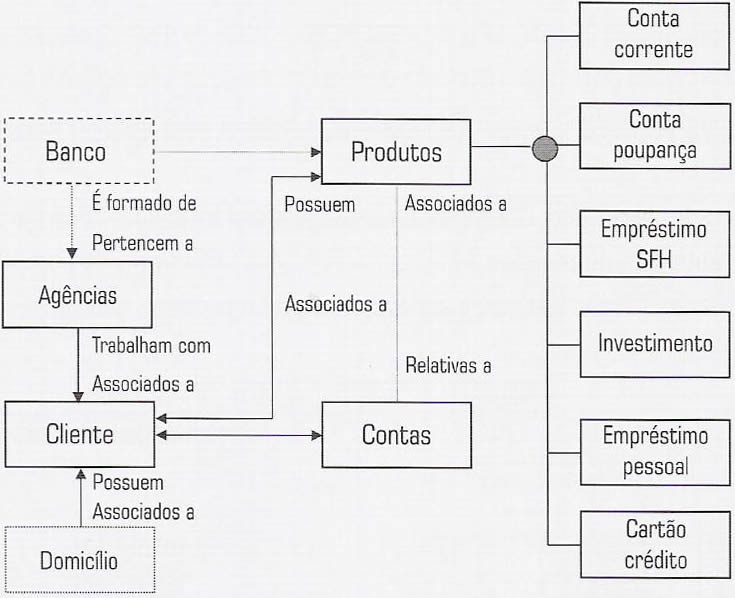
\includegraphics[width=9.063cm,height=7.359cm]{monograph-img002.jpg} \textsf{\MakeUppercase{ \newline
FIGURA }}\textsf{3: Exemplo de um modelo relacional ou tradicional.}}

{\selectlanguage{portuges}\sffamily
Fonte: BARBIERI, 2001, p. 107.}

{\selectlanguage{portuges}
 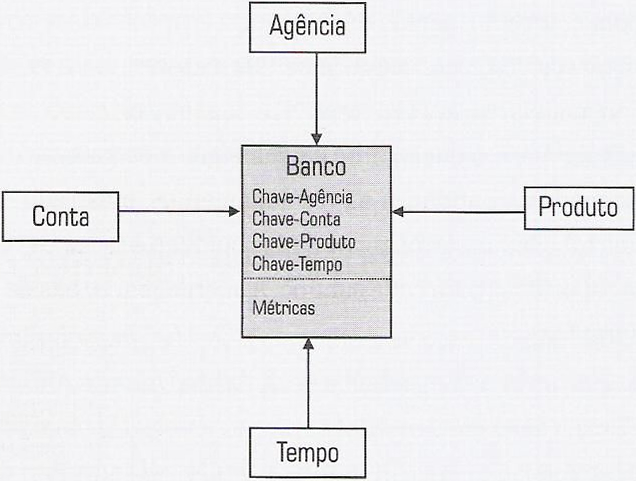
\includegraphics[width=9.417cm,height=7.121cm]{monograph-img003.jpg} \textsf{\MakeUppercase{\newline
FIGURA }}\textsf{4: Exemplo de um modelo dimensional.}}


\bigskip

{\selectlanguage{portuges}\sffamily
Barbieri compara (2001, p. 38), no quadro 3, a vis\~ao dimensional (modelo dimensional) com a estrutura tradicional
(modelo relacional).}


\bigskip

{\selectlanguage{portuges}
\textsf{Fonte: BARBIERI, 2001, p. 108.\newline
} 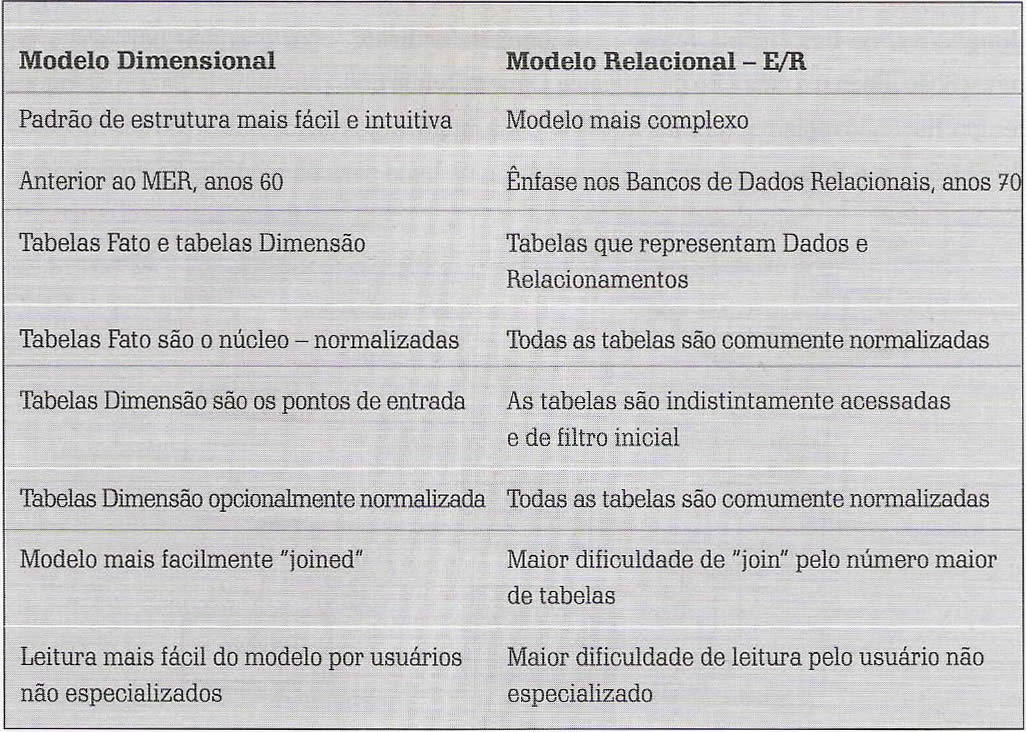
\includegraphics[width=12.065cm,height=8.597cm]{monograph-img004.jpg} \textsf{\MakeUppercase{ \newline
QUADRO }}\textsf{3: Compara\c{c}\~ao entre modelo relacional e modelo dimensional. }}

{\selectlanguage{portuges}\sffamily
Fonte: BARBIERI, 2001, p. 38. }

{\selectlanguage{portuges}
\textsf{A partir deste modelo tem-se aberta a possibilidade de melhor transposi\c{c}\~ao dos dados e capta\c{c}\~ao das
informa\c{c}\~oes para elaborar um melhor caminho para o suporte \`a decis\~ao. Barbieri diz que (2001, p. 48-49) o
conceito de BI deve ser entendido como o processo de desenvolvimento de: Estruturas especiais de armazenamento de
informa\c{c}\~oes como Data Warehouse (DW), Data Marts (DM) e ODS (Operational Data Store), com o objetivo de se montar
uma base de recursos informacionais, capaz de sustentar a camada de intelig\^encia da empresa e pass\'ivel de ser
aplicada aos seus neg\'ocios, como elementos diferenciais e competitivos e aplica\c{c}\~oes especiais de tratamentos
desses dados, como OLAP e Data Mining.}}

{\selectlanguage{portuges}
\textsf{Data warehouse, ou armaz\'em de dados, \'e um banco de dados, destinado a sistemas de apoio \`a decis\~ao e
cujos dados foram armazenados em estruturas l\'ogicas dimensionais, possibilitando o seu processamento anal\'itico por
ferramentas especiais (OLAP -- Processamento anal\'itico on-line e Mining - Minera\c{c}\~ao). Estes bancos de dados,
utilizando o modelo de estrutura dimensional s\~ao vitais para a elabora\c{c}\~ao e desenvolvimento do sistema de apoio
\`a decis\~ao, uma vez que implantam a transforma\c{c}\~ao na forma de transpor os dados, proposta pelo modelo
dimensional (BARBIERI, 2001, p. 49). }}

{\selectlanguage{portuges}\sffamily
Data warehouses foram propostos para melhor responderem a demandas crescentes de tomadores de decis\~ao. Um data
warehouse \'e uma cole\c{c}\~ao de dados baseados em assuntos, integrados, n\~ao-vol\'ateis e vari\'aveis em
rela\c{c}\~ao ao tempo para apoiar decis\~oes gerenciais (MALINOWSKI; ZIM\'ANYI, 2008, p. 41).}

{\selectlanguage{portuges}
\textsf{Malinowski e Zim\'anyi (2008, p. 41-42) descrevem os aspectos do data warehouse, ilustrados por Inmon nas
Figuras 5 (1997, p. 34), 6 (1997, p. 35), 7 (1997, p. 36) e 8 (1997, p. 37), da seguinte forma:}}

\liststyleWWviiiNumxii
\begin{enumerate}
\item {\selectlanguage{portuges}
\textsf{Baseado em assunto significa que data warehouses t\^em foco em demandas anal\'iticas de gerentes em v\'arios
n\'iveis do processo decis\'orio. Estes assuntos variam dependendo dos tipos de atividades ou neg\'ocios realizados
pela organiza\c{c}\~ao. Isto se diferencia da modelagem tradicional, onde o foco est\'a em fun\c{c}\~oes espec\'ificas
que as aplica\c{c}\~oes precisam realizar. Em uma organiza\c{c}\~ao, muitos assuntos anal\'iticos podem ser inclu\'idos
num mesmo data warehouse. }}
\end{enumerate}
 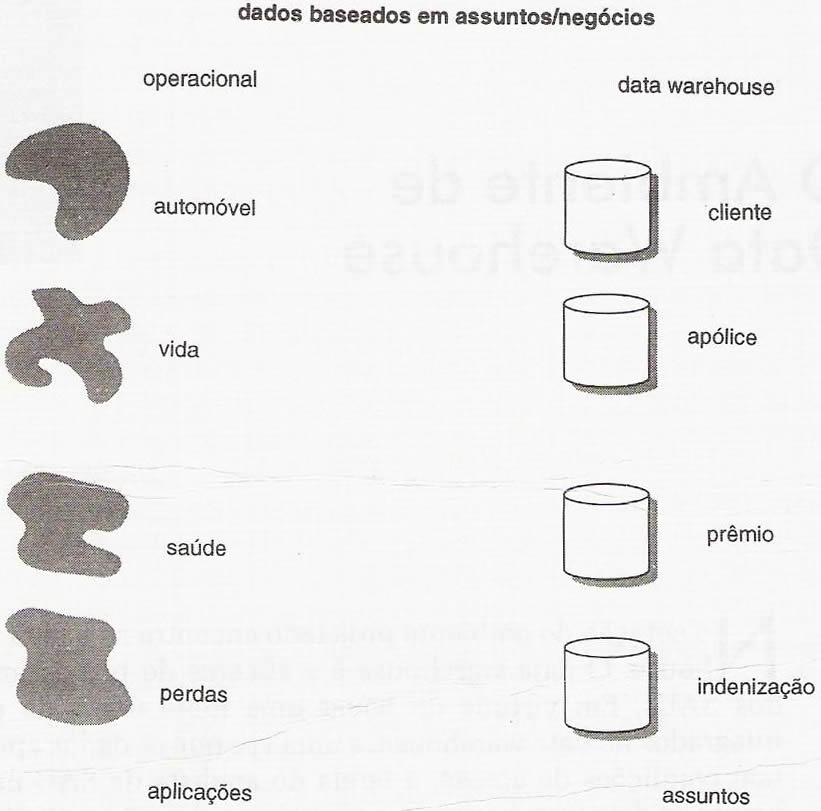
\includegraphics[width=8.174cm,height=8.073cm]{monograph-img005.jpg} 

{\selectlanguage{portuges}
\textsf{\MakeUppercase{FIGURA }}\textsf{5: Um exemplo de dados baseados em assuntos/neg\'ocios. }}

{\selectlanguage{portuges}
\textsf{Fonte: INMON, 1997, p. 34. \ }}

\liststyleWWviiiNumxii
\setcounter{saveenum}{\value{enumi}}
\begin{enumerate}
\setcounter{enumi}{\value{saveenum}}
\item {\selectlanguage{portuges}
\textsf{Integrado representa a complexa uni\~ao entre dados de diversos sistemas internos e externos, o que implica em
solucionar problemas na defini\c{c}\~ao dos dados e nos conte\'udos, como formato de dados e codifica\c{c}\~ao de
dados, sin\^onimos (campos com nomes diferentes mas com mesmos dados), hom\^onimos (campos com mesmos nomes por\'em com
diferentes significados), multiplicidade de ocorr\^encia de dados, dentre muitos outros. }}
\end{enumerate}
 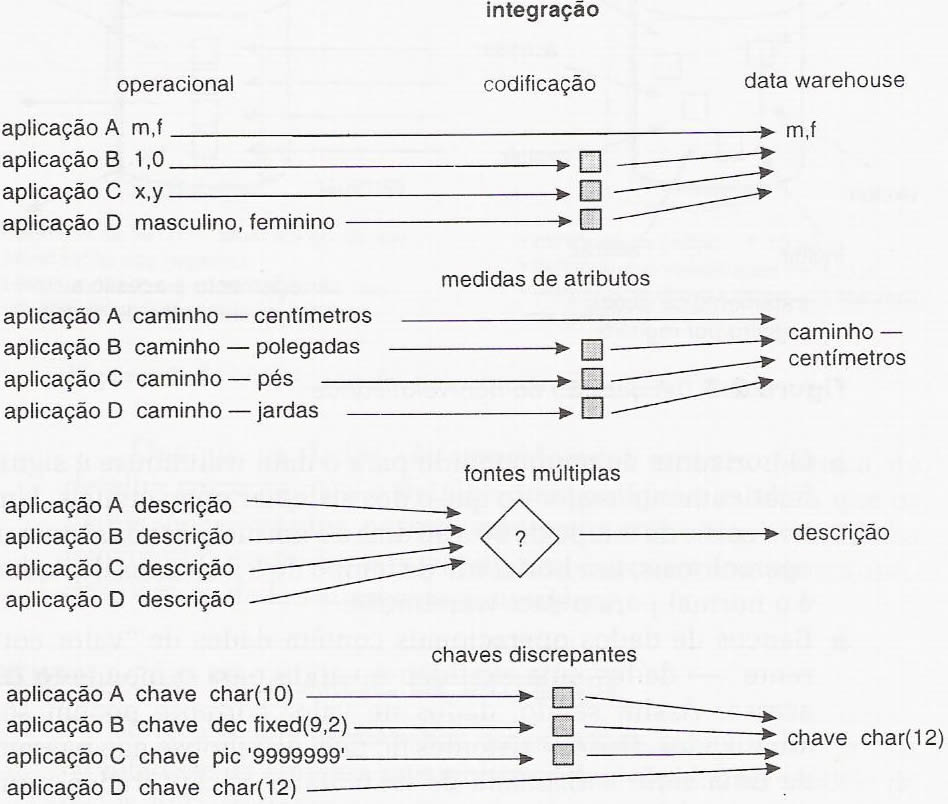
\includegraphics[width=10.739cm,height=9.118cm]{monograph-img006.jpg} 

{\selectlanguage{portuges}
\textsf{\MakeUppercase{FIGURA }}\textsf{6: A quest\~ao da integra\c{c}\~ao. }}

{\selectlanguage{portuges}
\textsf{Fonte: INMON, 1997, p. 34. \ }}

\liststyleWWviiiNumxii
\setcounter{saveenum}{\value{enumi}}
\begin{enumerate}
\setcounter{enumi}{\value{saveenum}}
\item {\selectlanguage{portuges}
\textsf{N\~ao-vol\'atil significa que a durabilidade dos dados \'e concedida pelo bloqueio na modifica\c{c}\~ao e na
remo\c{c}\~ao dos dados, que expandem o escopo dos dados para um per\'iodo de tempo muito maior do que o de um sistema
de processamento de transa\c{c}\~oes. Um data warehouse armazena dados durante muitos anos, comumente entre 5 a 10 anos
ou mais, enquanto num sistema de processamento de transa\c{c}\~oes os dados ficam dispon\'iveis por um per\'iodo curto
de tempo, por exemplo, de 2 a 6 meses, por serem necess\'arios para opera\c{c}\~oes di\'arias e que podem ser
sobrescritos quando necess\'ario. }}
\end{enumerate}
 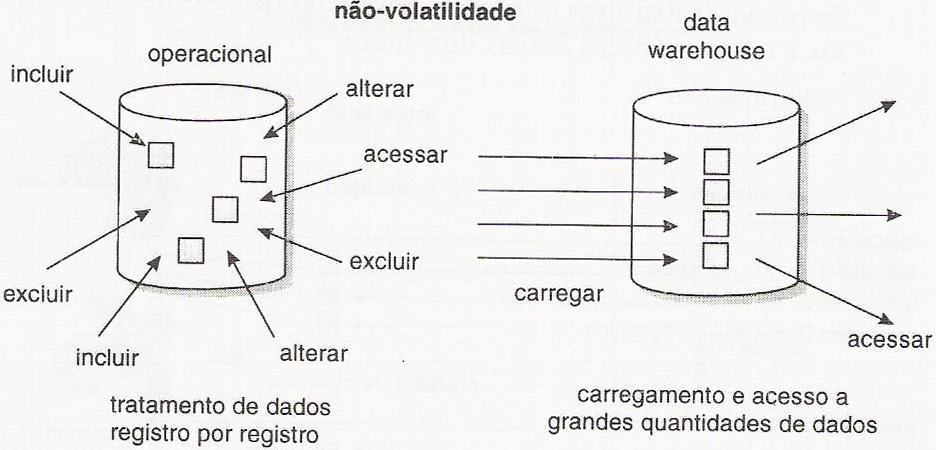
\includegraphics[width=11.91cm,height=5.731cm]{monograph-img007.jpg} 

{\selectlanguage{portuges}
\textsf{\MakeUppercase{FIGURA }}\textsf{7: A quest\~ao da n\~ao-volatidade. }}

{\selectlanguage{portuges}
\textsf{Fonte: INMON, 1997, p. 34. \ }}

\liststyleWWviiiNumxii
\setcounter{saveenum}{\value{enumi}}
\begin{enumerate}
\setcounter{enumi}{\value{saveenum}}
\item {\selectlanguage{portuges}
\textsf{Vari\'aveis em rela\c{c}\~ao ao tempo indica a possibilidade de possuir diferentes valores para a mesma
informa\c{c}\~ao, e o tempo quando a mudan\c{c}a para estes valores ocorreu. Em contraste, um banco de dados
operacional ou tradicional pode n\~ao ter suporte expl\'icito ao tempo, uma vez que isto n\~ao \'e necess\'ario para as
aplica\c{c}\~oes do dia-a-dia ou \'e dif\'icil de implementar.}}
\end{enumerate}
 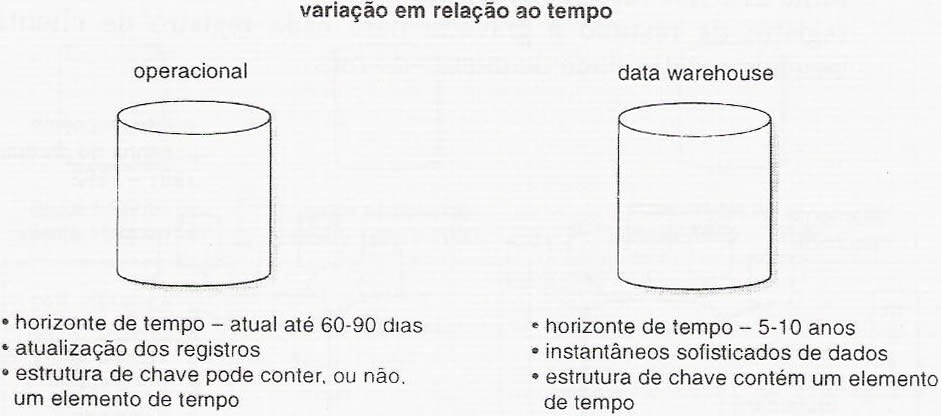
\includegraphics[width=11.77cm,height=5.203cm]{monograph-img008.jpg} 

{\selectlanguage{portuges}
\textsf{\MakeUppercase{FIGURA }}\textsf{8: A quest\~ao da varia\c{c}\~ao em rela\c{c}\~ao ao tempo. }}

{\selectlanguage{portuges}
\textsf{Fonte: INMON, 1997, p. 34. \ }}

{\selectlanguage{portuges}
\textsf{Data warehouses s\~ao baseados num modelo multidimensional. Este modelo permite um melhor entendimento de dados
para prop\'ositos anal\'iticos e garante melhor desempenho para consultas anal\'iticas complexas. O modelo
multidimensional visualiza os dados num espa\c{c}o de }\textsf{\textit{n}}\textsf{{}-dimens\~oes, usualmente chamado de
cubo de dados ou hipercubo (MALINOWSKI; ZIM\'ANYI, 2008, p. 43).}}

{\selectlanguage{portuges}
\textsf{A Figura 9, segundo Malinowski e Zim\'anyi (2008, p. 43), ilustra um cubo tri-dimensional de dados de venda que
possui as dimens\~oes Loja (Store), Tempo (Time) e Produto (Product), e o fato de valores medidos (measure values), no
caso, quantidade de vendas.}}


\bigskip

{\selectlanguage{portuges}
 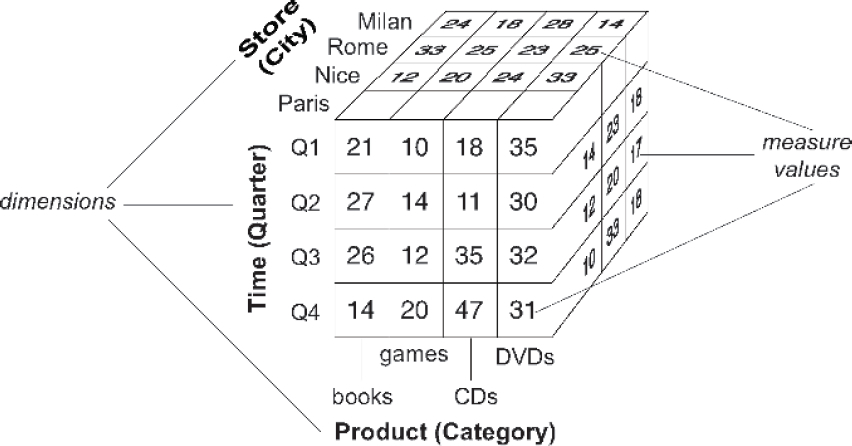
\includegraphics[width=11.18cm,height=5.853cm]{monograph-img009.jpg} \textsf{\MakeUppercase{ }}}

{\selectlanguage{portuges}
\textsf{\MakeUppercase{FIGURA }}\textsf{9: Cubo tri-dimensional de dados de venda que possui as dimens\~oes Loja
(Store), Tempo (Time) e Produto (Product), e o fato de valores medidos (measure values).}}

{\selectlanguage{portuges}
\textsf{Fonte: MALINOWSKI; ZIM\'ANYI, 2008, p. 43.}}


\bigskip

\liststyleWWviiiNumi
\begin{enumerate}
\item \begin{enumerate}
\item {\selectlanguage{portuges}\sffamily
MODELAGEM DE UM SISTEMA DE BI}
\end{enumerate}
\end{enumerate}
{\selectlanguage{portuges}\sffamily
Nesta se\c{c}\~ao ser\~ao abordadas as etapas e a estrutura de constru\c{c}\~ao de um sistema de BI.}


\bigskip

\liststyleWWviiiNumi
\setcounter{saveenum}{\value{enumi}}
\begin{enumerate}
\setcounter{enumi}{\value{saveenum}}
\item \setcounter{saveenum}{\value{enumii}}
\begin{enumerate}
\setcounter{enumii}{\value{saveenum}}
\item \setcounter{saveenum}{\value{enumiii}}
\begin{enumerate}
\setcounter{enumiii}{\value{saveenum}}
\item {\selectlanguage{portuges}\sffamily\bfseries
Etapas para constru\c{c}\~ao de um Sistema de BI}
\end{enumerate}
\end{enumerate}
\end{enumerate}
{\selectlanguage{portuges}
\textsf{Para a constru\c{c}\~ao e implanta\c{c}\~ao de um Sistema de BI, Barbieri (2001, p. 68) afirma que os principais
passos para tal s\~ao Planejamento, Levantamento de Necessidades, Modelagem Dimensional, Projeto F\'isico dos Bancos de
Dados, Projeto de Transforma\c{c}\~ao, Desenvolvimento de Aplica\c{c}\~oes, Valida\c{c}\~ao e Teste, Treinamento e
Implanta\c{c}\~ao.}}

{\selectlanguage{portuges}
\textsf{As etapas para o planejamento de um Sistema de BI s\~ao descritos por Barbieri (2001, p. 69-73) da seguinte
forma:}}

\liststyleWWviiiNumxxv
\begin{enumerate}
\item {\selectlanguage{portuges}\sffamily
Foco no neg\'ocio. Nessa etapa, a primeira do projeto de DW/DM, objetiva-se definir o escopo do projeto, atentando-se
para as \'areas cr\'iticas da empresa e as necessidades mais prementes de informa\c{c}\~oes gerenciais, como, por
exemplo, a melhoria de competitividade, ou a prospec\c{c}\~ao de novos mercados. O ambiente de Clientes surge,
indiscutivelmente, como primeiro candidato natural a um projeto de DW/DM, principalmente agora, quando cresce com
efervesc\^encia o conceito de ERM/CRM. Associado a Cliente, aparecem Marketing, Finan\c{c}as, etc., como \'areas
tamb\'em fortemente vocacionadas para os projetos subseq\"uentes de BI.}
\item {\selectlanguage{portuges}
\textsf{Defini\c{c}\~ao da abordagem. Essa defini\c{c}\~ao diz respeito \`a abordagem corporativa escolhida para os
projetos de DW/DM. Basicamente consiste na escolha entre um `}\textsf{\textit{approach}}\textsf{{}' que define um DW
monol\'itico, grande, fortemente integrado em n\'ivel de projeto, no qual sair\~ao os DM na medida de suas
implementa\c{c}\~oes. As considera\c{c}\~oes a respeito dessas alternativas passam pelos aspectos de maior
integra\c{c}\~ao e pela disponibiliza\c{c}\~ao mais imediata dos produtos requeridos.}}
\item {\selectlanguage{portuges}
\textsf{Planejamento para integra\c{c}\~ao. Definidas as \'areas/assuntos do primeiro projeto, parte-se para estabelecer
uma vis\~ao que permita amarr\'a-las, na medida em que as implementa\c{c}\~oes forem realizadas separadamente. Isso, no
fundo, significa ter, em um n\'ivel razo\'avel, as principais dimens\~oes requeridas e as m\'etricas (dados) para que
esses projetos possam ser coerentemente alinhavados. Isso n\~ao \'e uma tarefa trivial, pois poder\'a envolver um
trabalho de levantamento e an\'alise, mesmo que introdut\'orio, de v\'arias \'areas, podendo estender o cronograma de
desenvolvimento do trabalho. O ideal aqui \'e conseguir estabelecer um meio termo entre o desenvolvimento gradual de
DW/DM e a defini\c{c}\~ao de dimens\~oes com formas e m\'etricas compat\'iveis, que permitam a integra\c{c}\~ao
gradativa dos DW/DM, sem agigantamento de projetos. A id\'eia \'e de se garimpar as dimens\~oes que ser\~ao demandadas
em cada \'area de neg\'ocios da empresa, observando-se, nessas dimens\~oes, a sua sem\^antica (o que ela significa)
para aquele contexto, os seus atributos e as suas hierarquiza\c{c}\~oes. Isso permitir\'a o mapeamento de dimens\~oes
em conformidade, o que significa que os elos entre os DM estar\~ao identificados e possibilitar\~ao as conex\~oes
futuras e integra\c{c}\~oes sem grandes traumas. }}
\item {\selectlanguage{portuges}
\textsf{Defini\c{c}\~ao da arquitetura tecnol\'ogica. Antes de se iniciar o projeto de DW/DM deve-se atentar para a
arquitetura tecnol\'ogica que servir\'a de base para o projeto. \'E fundamental que os componentes b\'asicos da
arquitetura sejam definidos antes do in\'icio do projeto do DW/DM, pois fatores relacionados \`a performance e
disponibilidade podem definir n\'iveis de servi\c{c}os e graus de compromissos variados durante o projeto. Os
componentes tecnol\'ogicos b\'asicos, que dever\~ao }\textsf{ser observados, al\'em da rede corporativa s\~ao: Sistema
Gerenciador de Banco de Dados; Ferramentas de Desenvolvimento de Sistemas OLAP e Mining; Ferramentas para Processos de
Extra\c{c}\~ao, Transforma\c{c}\~ao e Carga; Cat\'alogo para controle de Metadados; Mecanismos para Transfer\^encia de
Dados entre ambientes heterog\^eneos; Servidor de Data Mart/Cubos; e Extrato de Dados para Data Mining.}}
\end{enumerate}
{\selectlanguage{portuges}
\textsf{Al\'em do planejamento, Barbieri descreve (2001, p. 73-77) os outros oito passos para a constru\c{c}\~ao de um
Sistema de BI:}}

\liststyleWWviiiNumxxxvi
\begin{enumerate}
\item {\selectlanguage{portuges}
\textsf{Levantamento de necessidades. Nesta etapa dever\~ao ser identificados os modelos dimensionais, ou aquele que
representa os blocos conceituais de dados necess\'arios ao alcance dos objetivos do sistema de suporte a decis\~ao e
outro modelo que \'e relacionado com as fontes das informa\c{c}\~oes, chamado de Fonte dos Dados, que nele, dever\~ao
ser registrados os blocos conceituais de dados existentes, com suas respectivas descri\c{c}\~oes e formas atuais de
armazenamento e de uso nos sistemas, e que provavelmente habitam os variados ambientes operacionais da instala\c{c}\~ao
ou as fontes externas de dados;}}
\item {\selectlanguage{portuges}
\textsf{Modelagem dimensional. Os dados, quando analisados sob a \'otica desta modelagem, dever\~ao passar por
observa\c{c}\~oes nem sempre percebidas em um projeto de Banco de Dados convencional, como com o maior n\'ivel de
granularidade ou detalhe;}}
\item {\selectlanguage{portuges}
\textsf{Projeto f\'isico dos bancos de dados. Ser\~ao desenhadas as estruturas l\'ogicas do modelo dimensional, com as
defini\c{c}\~oes de tabelas Fatos e tabelas Dimens\~ao, relacionamentos, indexa\c{c}\~ao, atributos de tabelas e
implanta\c{c}\~ao de regras; }}
\item {\selectlanguage{portuges}
\textsf{Projeto de Extra\c{c}\~ao, Transforma\c{c}\~ao e Carga. A descri\c{c}\~ao detalhada desta etapa ser\'a explanada
ainda nesta subse\c{c}\~ao;}}
\item {\selectlanguage{portuges}\sffamily
Desenvolvimento de aplica\c{c}\~oes, onde ser\'a projetado o sistema aplicativo, objeto do trabalho;}
\item {\selectlanguage{portuges}\sffamily
Valida\c{c}\~ao e teste. Fase em que o sistema \'e testado considerando-se, o m\'aximo poss\'ivel, as simula\c{c}\~oes
de volume e de processamentos;}
\item {\selectlanguage{portuges}\sffamily
Treinamento. O grupo objeto do treinamento dever\'a ser formado prioritariamente pelos usu\'arios voltados para as
atividades de neg\'ocios, al\'em dos gerentes das \'areas envolvidas;}
\item {\selectlanguage{portuges}\sffamily
Implanta\c{c}\~ao. A implanta\c{c}\~ao dever\'a ser seguida de um rigoroso acompanhamento de uso das aplica\c{c}\~oes
disponibilizadas.}
\end{enumerate}
{\selectlanguage{portuges}
\textsf{Para a constru\c{c}\~ao de um projeto de DW, precisaremos construir uma estrutura de Extra\c{c}\~ao,
Transforma\c{c}\~ao e Carga (do ingl\^es }\textsf{\textit{Extract Transform Load}}\textsf{ }\textsf{\textit{{}-
ETL}}\textsf{), onde ``dever\~ao ser definidos os processos requeridos de transforma\c{c}\~ao do modelo fonte para o
modelo Dimensional'' (BARBIERI, 2001, p. 74). A seguir, segundo conceitua Barbieri (2001, p.75), seguem as divis\~oes
da extra\c{c}\~ao e tratamento dos dados:}}

\liststyleWWviiiNumxi
\begin{enumerate}
\item {\selectlanguage{portuges}\sffamily
Filtro de Dados. Relaciona os procedimentos e condi\c{c}\~oes para se eliminar os elementos de dados indesej\'aveis no
modelo Dimensional.}
\item {\selectlanguage{portuges}\sffamily
Integra\c{c}\~ao de Dados. Define a forma de se correlacionar informa\c{c}\~oes existentes em fontes distintas, e que
dever\~ao ser integradas no sistema gerencial.}
\item {\selectlanguage{portuges}\sffamily
Condensa\c{c}\~ao de Dados. Define forma de se reduzir volumes de dados visando obter informa\c{c}\~oes resumidas e
sumariadas.}
\item {\selectlanguage{portuges}\sffamily
Convers\~ao de Dados. Define os procedimentos para se transformar dados em unidades, formatos e dimens\~oes diferentes.}
\item {\selectlanguage{portuges}\sffamily
Deriva\c{c}\~ao de Dados. Define os meios e f\'ormulas para se produzir dados virtuais, a partir de dados existentes.}
\end{enumerate}
{\selectlanguage{portuges}\sffamily
Date define (2004, p. 600-602) cada opera\c{c}\~ao de obten\c{c}\~ao e prepara\c{c}\~ao dos dados da seguinte forma:}

\liststyleWWviiiNumxxvi
\begin{enumerate}
\item {\selectlanguage{portuges}\sffamily
Extra\c{c}\~ao. \'E o processo de capturar dados de bancos de dados operacionais (tradicionais) e outras fontes. O
processo de extra\c{c}\~ao tende a ser muito intenso em termos de Entrada/Sa\'ida, e assim pode interferir com
opera\c{c}\~oes de miss\~ao cr\'itica; por essa raz\~ao, ela normalmente \'e realizada em paralelo -- isto \'e, como um
conjunto de subprocessos paralelos -- e em n\'ivel f\'isico.}
\item {\selectlanguage{portuges}\sffamily
Limpeza. Poucas fontes de dados controlam a qualidade dos dados de forma adequada. Como resultado, os dados normalmente
exigem limpeza antes de poderem ser introduzidos no banco de dados de apoio \`a decis\~ao. As opera\c{c}\~oes t\'ipicas
de limpeza incluem o preenchimento de valores omitidos, a corre\c{c}\~ao de erros de digita\c{c}\~ao e outros erros de
entrada de dados, o estabelecimento de abrevia\c{c}\~oes e formatos padronizados, a substitui\c{c}\~ao de sin\^onimos
por identificadores padr\~ao, e assim por diante. Os dados reconhecidos como errados e que n\~ao podem ser limpos s\~ao
rejeitados.}
\item {\selectlanguage{portuges}\sffamily
Transforma\c{c}\~ao e consolida\c{c}\~ao. Mesmo depois de terem sido limpos, os dados provavelmente ainda n\~ao
estar\~ao na forma que o sistema de apoio \`a decis\~ao, no caso do escopo deste trabalho, o SIG, exige, e por isso
precisar\~ao ser transformados de modo apropriado. Em geral, a forma exigida ser\'a um conjunto de arquivos, um para
cada tabela identificada no esquema f\'isico; como resultado, a transforma\c{c}\~ao de dados pode envolver a divis\~ao
e/ou a combina\c{c}\~ao de registros de origem. Por quest\~oes de desempenho, opera\c{c}\~oes de transforma\c{c}\~ao
costumam ser executadas em paralelo. A transforma\c{c}\~ao \'e particularmente importante quando v\'arias origens de
dados precisam ser mescladas, em um processo chamado consolida\c{c}\~ao. Nesse caso, quaisquer relacionamentos
impl\'icitos entre dados de origens distintas precisam se tornar expl\'icitos. Al\'em disso, datas e horas associadas
com o significado comercial dos dados precisam ser mantidas e correlacionadas entre as origens, um processo que se
chama `sincroniza\c{c}\~ao de tempo'.}
\item {\selectlanguage{portuges}\sffamily
Carga. Considera-se que as `opera\c{c}\~oes de carga' incluem mover os dados transformados e consolidados para o banco
de dados de apoio \`a decis\~ao, verificar a consist\^encia dos dados (isto \'e, fazer a verifica\c{c}\~ao da
integridade) e construir quaisquer \'indices necess\'arios.}
\item {\selectlanguage{portuges}\sffamily
Renova\c{c}\~ao. A maioria dos bancos de dados de apoio \`a decis\~ao exige renova\c{c}\~ao peri\'odica dos dados, a fim
de mant\^e-los razoavelmente atualizados. Em geral, a renova\c{c}\~ao envolve uma carga parcial, embora algumas
aplica\c{c}\~oes de apoio \`a decis\~ao exijam que se descarte tudo no banco de dados e se fa\c{c}a o recarregamento
completo dos dados. A renova\c{c}\~ao envolve todos os problemas associados com a carga, mas tamb\'em pode ser
necess\'ario executa-la enquanto os usu\'arios est\~ao acessando o banco de dados.}
\end{enumerate}

\bigskip

\liststyleWWviiiNumi
\begin{enumerate}
\item \begin{enumerate}
\item \begin{enumerate}
\item {\selectlanguage{portuges}\sffamily\bfseries
Armazenamento de Dados}
\end{enumerate}
\end{enumerate}
\end{enumerate}
{\selectlanguage{portuges}
\textsf{Os bancos de dados tradicionais n\~ao satisfazem ao requisito crescente de an\'alise de dados por parte das
organiza\c{c}\~oes. Eles suportam as opera\c{c}\~oes di\'arias de uma organiza\c{c}\~ao e seu foco principal \'e
garantir acessos r\'apidos aos dados num ambiente de m\'ultiplos usu\'arios que necessitam de processamento de
transa\c{c}\~oes. Estes sistemas s\~ao conhecidos como bancos de dados operacionais ou sistemas de processamento de
transa\c{c}\~oes online (OLTP - do ingl\^es }\textsf{\textit{online transaction processing}}\textsf{) e, normalmente,
cont\^em dados detalhados, n\~ao cont\^em dados hist\'oricos, e em sua maioria s\~ao altamente normalizados, possuem um
desempenho ruim quando executam consultas complexas que precisam unir muitas tabelas relacionais ou agregar largos
volumes de dados (MALINOWSKI; ZIM\'ANYI, 2008, p. 41).}}

{\selectlanguage{portuges}
\textsf{Conforme visto na subse\c{c}\~ao 2.3.5, o data warehouse \'e uma solu\c{c}\~ao eficiente para armazenamento dos
dados de forma concisa e confi\'avel sobre opera\c{c}\~oes coerentes, tend\^encias e mudan\c{c}as relativas \`a
empresa.}}

{\selectlanguage{portuges}
\textsf{De in\'icio a constru\c{c}\~ao de data warehouse pressupunha um projeto integrado, monol\'itico, onde um modelo
\'unico contemplaria, com detalhes, todas as informa\c{c}\~oes ``fato'' e suas respectivas ``dimens\~oes''. Isso
significava modelar grande parte da empresa (ou a sua totalidade). Depois de pronto o grande dep\'osito, seriam criados
a partir dele, os data marts, ou mercados de dados espec\'ificos para cada espa\c{c}o de neg\'ocios da empresa. Os
projetos de data warehouse, elaborados nessa linhagem, come\c{c}aram a demorar mais do que o suportado pelas
ger\^encias reprimidas pela aus\^encia cr\^onica de informa\c{c}\~oes para decidir (BARBIERI, 2001, p. 54-55).}}

{\selectlanguage{portuges}
\textsf{Sobre os data marts, Laudon e Laudon (2007, p. 150) dizem que empresas podem criar armaz\'ens menores que os
data warehouses, que possuem \^ambito empresarial nos quais um armaz\'em central de dados atende \`a organiza\c{c}\~ao
inteira, e estes }\textsf{armaz\'ens menores s\~ao denominados data marts. Data mart \'e um subconjunto de um data
warehouse, no qual uma por\c{c}\~ao resumida ou altamente focalizada dos dados da organiza\c{c}\~ao \'e colocada em um
banco separado destinado a uma popula\c{c}\~ao espec\'ifica de usu\'arios. Um data mart em geral focaliza uma \'unica
\'area de interesse ou linha de neg\'ocios, de modo que pode ser montado com mais rapidez a um custo mais baixo do que
um data warehouse de \^ambito empresarial.}}

{\selectlanguage{portuges}\sffamily
Segundo Date (2004, p. 604), pode-se resumir data mart como um dep\'osito de dados especializado, orientado por assunto,
integrado, vol\'atil e vari\'avel no tempo, que fornece apoio a um subconjunto espec\'ifico de decis\~oes da
ger\^encia. As principais distin\c{c}\~oes entre um data mart e um data warehouse s\~ao as de que um data mart \'e
especializado e vol\'atil. Por especializado, sabe-se que ele cont\'em dados para apoio somente a uma \'area
espec\'ifica; por vol\'atil, sabe-se que os usu\'arios podem atualizar os dados, e talvez at\'e mesmo criar novos dados
(ou seja, novas tabelas) para alguns prop\'ositos.}

{\selectlanguage{portuges}
\textsf{Date descreve tr\^es t\'ecnicas principais para a cria\c{c}\~ao de um data mart (2004, p. 604):}}

\liststyleWWviiiNumxxviii
\begin{enumerate}
\item {\selectlanguage{portuges}
\textsf{Os dados podem simplesmente ser extra\'idos do data warehouse -- com efeito, seguindo uma t\'atica de `dividir e
conquistar' para a carga de trabalho global de apoio \`a decis\~ao, a fim de obter melhor desempenho e escalabilidade.
Normalmente, os dados extra\'idos s\~ao carregados em um banco de dados com um esquema f\'isico muito semelhante ao
subconjunto aplic\'avel destinado ao data warehouse; contudo, pode ser poss\'ivel simplifica-lo um pouco, gra\c{c}as
\`a natureza especializada do data mart.}}
\item {\selectlanguage{portuges}
\textsf{Apesar do fato do data warehouse se destinar a fornecer um `\'unico ponto de controle', um data mart pode ainda
ser criado de modo independente (ou seja, n\~ao atrav\'es de extra\c{c}\~ao do data warehouse). Essa t\'ecnica poderia
ser apropriada se o data warehouse estivesse inacess\'ivel por alguma raz\~ao, digamos por quest\~oes financeiras,
operacionais, ou mesmo pol\'iticas (ou o data warehouse poderia nem sequer existir ainda).}}
\item {\selectlanguage{portuges}\sffamily
Algumas instala\c{c}\~oes seguiram uma abordagem de `data mart primeiro', na qual os data marts s\~ao criados conforme a
necessidade, com o data warehouse global sendo criado finalmente como uma consolida\c{c}\~ao dos diversos data marts.}
\end{enumerate}
{\selectlanguage{portuges}
\textsf{Tendo em vista a solu\c{c}\~ao apresentada pelo data warehouse frente ao OLTP, t\^em-se uma abordagem eficiente
para tratamento e processamento dos dados armazenados, que \'e o processamento anal\'itico online (OLAP -- do ingl\^es
}\textsf{\textit{online analytical processing}}\textsf{), que, segundo Laudon e Laudon (2007, p. 151), permite a
an\'alise multidimensional de dados, de forma que os usu\'arios vejam os mesmos dados de diferentes maneiras, pois usa
m\'ultiplas dimens\~oes, onde cada aspecto da informa\c{c}\~ao representa uma dimens\~ao diferente e permite que os
usu\'arios obtenham respostas online a quest\~oes espec\'ificas com uma velocidade razo\'avel, mesmo quando os dados
est\~ao armazenados em bancos de dados gigantescos, como n\'umeros de vendas de v\'arios anos.}}

{\selectlanguage{portuges}\sffamily
Segundo Date (2004, p. 607), OLAP pode ser definido como o processo interativo de criar, gerenciar, analisar e gerar
relat\'orios sobre dados.}

{\selectlanguage{portuges}
\textsf{O OLAP, de fato, deve ser descrito como ROLAP (`OLAP relacional'), por\'em acredita-se que MOLAP (`OLAP
multidimensional') seja uma forma melhor de abordagem do OLAP. O MOLAP envolve um banco de dados multidimensional, um
banco de dados no qual todos os dados est\~ao armazenados conceitualmente nas c\'elulas de um vetor multidimensional. O
sistema gerenciador de banco de dados (SGBD) de suporte \'e chamado de SGBD multidimensional (DATE, 2004, p.
612-613).}}

{\selectlanguage{portuges}
\textsf{O modelo multidimensional \'e comumente representado por tabelas relacionais organizadas em estruturas especiais
chamadas }\textsf{\textbf{modelagem estrela}}\textsf{ e }\textsf{\textbf{modelagem floco de neve}}\textsf{. Estas
modelagens relacionais associam uma tabela fato a v\'arias tabelas dimens\~ao (MALINOWSKI; ZIM\'ANYI, 2008, p. 4). }}

{\selectlanguage{portuges}
\textsf{Sobre modelagem estrela, Malinowski e Zim\'anyi (2008, p. 50) descrevem que existe apenas uma tabela fato
central, e uma gama de tabelas dimens\~ao para cada dimens\~ao. Em uma modelagem estrela, as tabelas dimens\~ao podem
conter redund\^ancia, especialmente junto a hierarquias: as tabelas n\~ao s\~ao necessariamente normalizadas.}}

{\selectlanguage{portuges}
\textsf{A Figura 10 exemplifica, segundo Poe, Klauer e Stephen (1998, p. 125), uma modelagem estrela para um Data
Warehouse de vendas.}}

{\selectlanguage{portuges}
 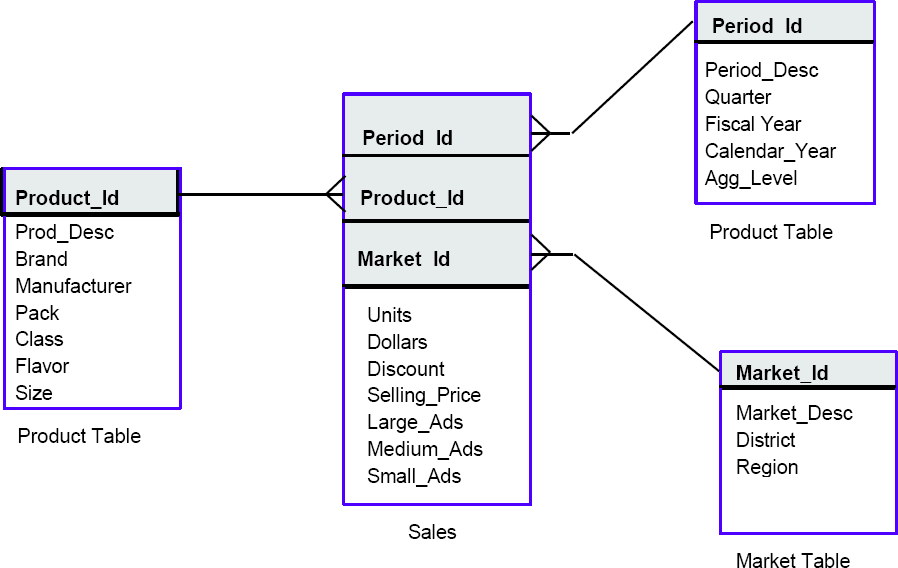
\includegraphics[width=12.386cm,height=7.833cm]{monograph-img010.jpg} \textsf{\MakeUppercase{ \newline
FIGURA }}\textsf{10: Modelagem estrela para um banco de dados de vendas, mostrando o relacionamento das chaves
prim\'arias. }}

{\selectlanguage{english}\sffamily
Fonte: POE; KLAUER; STEPHEN, 1998, p. 125. }

{\selectlanguage{portuges}
\textsf{Uma modelagem floco de neve evita a redund\^ancia de modelagens estrela, normalizando as tabelas dimens\~ao.
Portanto, uma dimens\~ao \'e representada por v\'arias tabelas relacionadas pela restri\c{c}\~ao de integridade
referencial. Al\'em disso, como no caso de modelagens estrela, a restri\c{c}\~ao de integridade referencial tamb\'em
relaciona a tabela fato e as tabelas dimens\~ao a um n\'ivel mais detalhado (MALINOWSKI; ZIM\'ANYI, 2008, p. 50). }}

{\selectlanguage{portuges}
\textsf{A Figura 11 demonstra um exemplo, segundo Poe, Klauer e Stephen (1998, p. 129), de uma modelagem floco de
neve.}}


\bigskip

{\selectlanguage{portuges}
 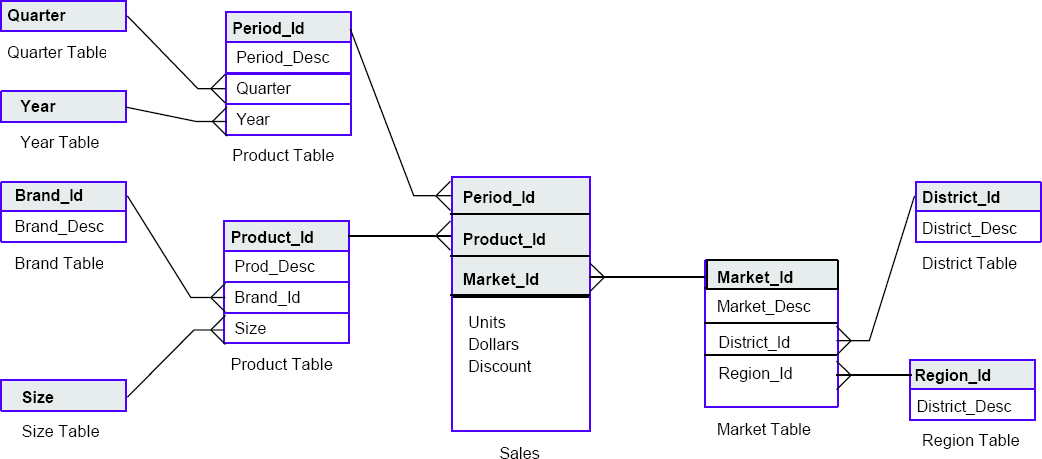
\includegraphics[width=13.012cm,height=5.715cm]{monograph-img011.jpg} \textsf{\MakeUppercase{ \newline
FIGURA }}\textsf{11: Uma modelagem floco de neve. }}

{\selectlanguage{english}\sffamily
Fonte: POE; KLAUER; STEPHEN, 1998, p. 129. }

{\selectlanguage{portuges}\sffamily
Barbieri define (2001, p. 174) que a estrat\'egia de armazenamento do data warehouse e data mart ou de seus cubos
extra\'idos permitem as seguintes op\c{c}\~oes:}

\liststyleWWviiiNumix
\begin{enumerate}
\item {\selectlanguage{portuges}
\textsf{ROLAP: Estrat\'egia onde s\~ao usados os pr\'oprios Sistemas de Gerenciamento de Bancos de Dados Relacionais
(SGBDR), com as tabelas sendo implementadas como estruturas relacionais cl\'assicas. Oferecem todas as vantagens de um
SGBDR, por\'em exigem um projeto cuidadoso do ponto de vista de performance, onde o excesso de tabelas normalizadas
poder\'a comprometer a performance das buscas. As tabelas b\'asicas e as vis\~oes ou cubos s\~ao armazenados no formato
de modelagem em estrela ou floco de neve.}}
\item {\selectlanguage{portuges}\sffamily
MOLAP: Estrat\'egia onde s\~ao usados gerenciadores de Bancos de Dados Propriet\'arios, com caracter\'isticas especiais
e ferramentas para tratamento dimensional de dados. Exigem a migra\c{c}\~ao dos dados do SGBD relacional para o
armazenamento multidimensional e a sua constante atualiza\c{c}\~ao. Podem ser limitados na sua capacidade m\'axima de
armazenamento, mas podem apresentar, em tese, melhor desempenho do que as outras alternativas por serem voltadas
exclusivamente para essas aplica\c{c}\~oes.}
\item {\selectlanguage{portuges}
\textsf{HOLAP (OLAP h\'ibrido): Representa uma abordagem de uso misto das duas estrat\'egias anteriores, onde as
estruturas relacionais s\~ao normalmente utilizadas para os dados de maior granularidade e as estruturas dimensionais
nativas s\~ao dedicadas ao armazenamento de agregados (menor granularidade).}}
\item {\selectlanguage{portuges}
\textsf{DOLAP (OLAP dimensional): Representa uma abordagem onde estruturas dimensionais ou relacionais, transferidas do
data warehouse ou do data mart para as esta\c{c}\~oes clientes, s\~ao armazenadas com o objetivo de facilitar a
performance de certas an\'alises, minimizando o tr\'afego de informa\c{c}\~oes entre o ambiente cliente e o ambiente
servidor.}}
\end{enumerate}

\bigskip

\liststyleWWviiiNumi
\begin{enumerate}
\item \begin{enumerate}
\item {\selectlanguage{portuges}\sffamily
FERRAMENTAS E TECNOLOGIAS PARA MONTAGEM DOS RELAT\'ORIOS}
\end{enumerate}
\end{enumerate}
{\selectlanguage{portuges}
\textsf{Ap\'os a concretiza\c{c}\~ao dos conceitos de data warehouse e de data mart, como forma de montagem de
dep\'ositos de dados, visando um consumo gerencial e voltada para tomadas de decis\~oes, surge a demanda pela
disponibiliza\c{c}\~ao das informa\c{c}\~oes contidas nestes data warehouses e data marts e, confome Malinowski e
Zim\'anyi (2008, p. 58), ``\'e nesta etapa que surgem ferramentas voltadas para o usu\'ario explorar estas
informa\c{c}\~oes, tais como ferramentas OLAP, ferramentas de relat\'orios, ferramentas de estat\'isticas e ferramentas
de minera\c{c}\~ao de dados''.}}

{\selectlanguage{portuges}
\textsf{Malinowski e Zim\'anyi ilustram (2008, p. 56), na Figura 12, uma arquitetura t\'ipica de funcionamento completo
de um sistema de BI. A primeira camada, de Fonte de Dados, comp\~oe-se Fontes Internas, Dados Operacionais e Fontes
Externas de dados. A segunda camada representa o processamento transparente de ETL e seu armazenamento de dados
tempor\'arios. A terceira camada representa o Data Warehouse, a qual comp\~oe-se do Data Warehouse, dos metadados deste
Data Warehouse e de seus respectivos Data Marts. A quarta camada representa o servidor OLAP e seus respectivos
metadados. Na quinta camada, de visualiza\c{c}\~ao, t\^em-se as ferramentas de data mining, ferramentas estat\'isticas,
ferramentas de gerenciamento de relat\'orios e ferramentas OLAP.}}

{\selectlanguage{portuges}
 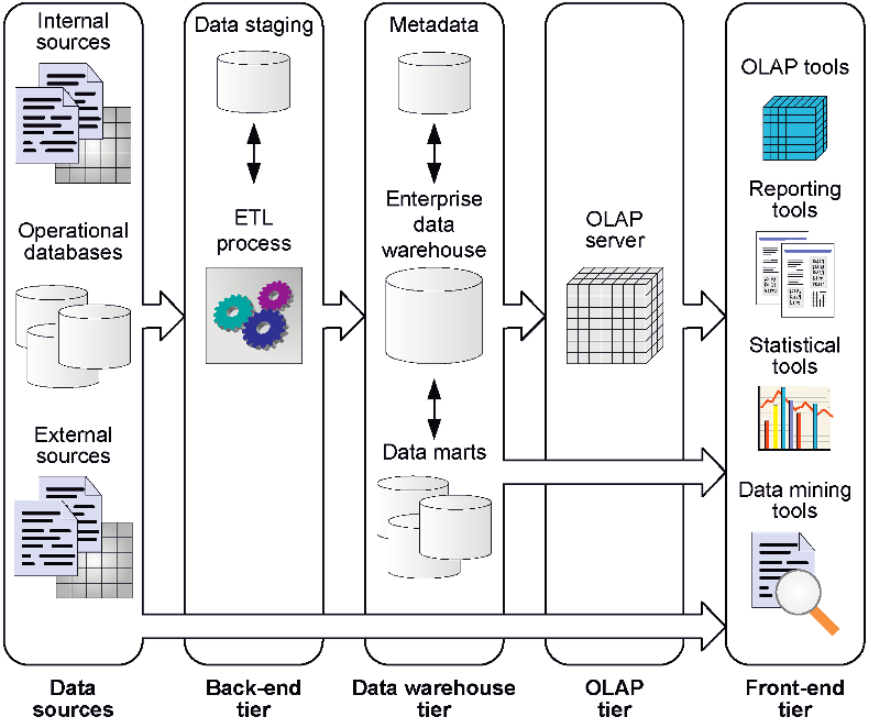
\includegraphics[width=14.102cm,height=11.684cm]{monograph-img012.jpg} \textsf{\MakeUppercase{ \newline
\newline
FIGURA }}\textsf{12: Arquitetura t\'ipica de um sistema de BI. }}

{\selectlanguage{portuges}
\textsf{Fonte: MALINOWSKI; ZIM\'ANYI, 2008, p. 56. }}

{\selectlanguage{portuges}
\textsf{As ferramentas OLAP permitem uma explora\c{c}\~ao interativa e manipula\c{c}\~ao dos dados contidos no data
warehouse com o objetivo de procurar padr\~oes e agrega\c{c}\~oes importantes para a organiza\c{c}\~ao. Elas facilitam
a formula\c{c}\~ao de consultas complexas que podem envolver grandes volumes de dados. As ferramentas de gerenciamento
de relat\'orios permitem a produ\c{c}\~ao, entrega e gerenciamento de relat\'orios, que podem ser em papel ou
interativos na Web. Relat\'orios usam consultas predefinidas, por exemplo, consultas que escolhem uma informa\c{c}\~ao
espec\'ifica num formato espec\'ifico que dever\'a ser realizado numa base regular. As ferramentas estat\'isticas s\~ao
utilizadas para analisar e visualizar o cubo de dados utilizando m\'etodos estat\'isticos. As ferramentas de Data
Mining permitem ao usu\'ario analisar dados com o objetivo de descobrir informa\c{c}\~oes valiosas, como padr\~oes e
tend\^encias; estas ferramentas tamb\'em permitem que se fa\c{c}am previs\~oes com base nos dados atuais. (MALINOWSKI;
ZIM\'ANYI, 2008, p. 58).}}


\bigskip

\liststyleWWviiiNumi
\setcounter{saveenum}{\value{enumi}}
\begin{enumerate}
\setcounter{enumi}{\value{saveenum}}
\item {\selectlanguage{portuges}
\textsf{\textbf{ESTUDO DE CASO: NIB FERRAGENS}}}
\end{enumerate}

\bigskip

{\selectlanguage{portuges}\sffamily
Este cap\'itulo aborda a estrutura atual da NIB Ferragens, os sistemas implantados atualmente, o que falta suprir na
\'area de vendas da empresa, o que um sistema de informa\c{c}\~oes gerenciais a ser implantado precisar\'a fornecer, a
proposta do desenvolvimento do sistema e os sistemas existentes no mercado que fornecem fun\c{c}\~oes semelhantes \`a
proposta. }


\bigskip

\liststyleWWviiiNumi
\setcounter{saveenum}{\value{enumi}}
\begin{enumerate}
\setcounter{enumi}{\value{saveenum}}
\item \setcounter{saveenum}{\value{enumii}}
\begin{enumerate}
\setcounter{enumii}{\value{saveenum}}
\item {\selectlanguage{portuges}\sffamily
NIB FERRAGENS}
\end{enumerate}
\end{enumerate}
{\selectlanguage{portuges}
\textsf{A NIB Ferragens come\c{c}ou em 20 de novembro de 1979 e atua no mercado de com\'ercio de ferragens, tendo como
principal fun\c{c}\~ao de neg\'ocio da empresa a gest\~ao das vendas. A empresa possui hoje sua matriz em Cariacica,
com 5.000 m{\texttwosuperior} de \'area f\'isica, e seis filiais, das quais compreendem a filial de Linhares, a filial
de Vila Velha, a filial de Aracruz, a filial de Iconha, a filial de Aimor\'es e a filial de Teixeira de Freitas (BA). O
faturamento da NIB Ferragens em 2011 foi de 30 milh\~oes de reais.}}

{\selectlanguage{portuges}
\textsf{A Figura 13 ilustra o organograma da empresa.}}


\bigskip

 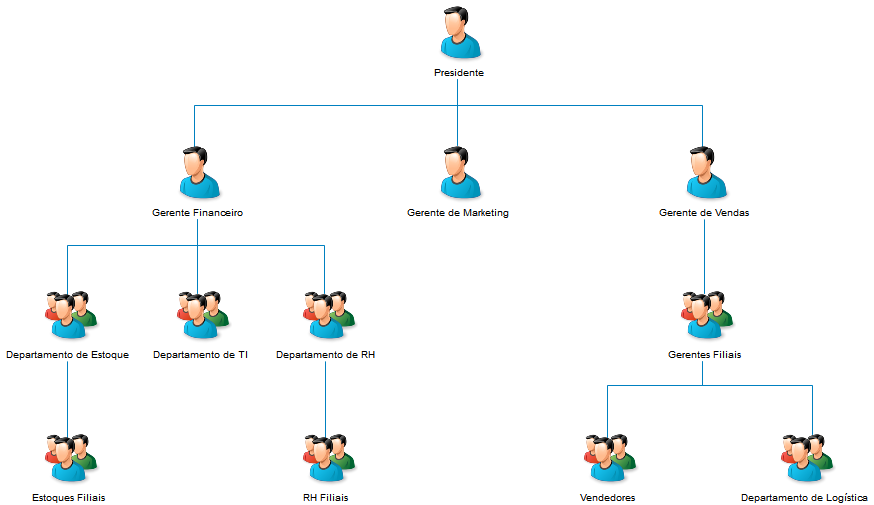
\includegraphics[width=15.981cm,height=9.234cm]{monograph-img013.png} 

{\selectlanguage{portuges}
\textsf{\MakeUppercase{\newline
FIGURA }}\textsf{13: Organograma da NIB Ferragens. }}


\bigskip

{\selectlanguage{portuges}
\textsf{Aliado \`a gest\~ao de vendas, correspondente \`a atividade principal do neg\'ocio da empresa, est\~ao a
gest\~ao de estoque, gest\~ao de log\'istica, gest\~ao financeira e gest\~ao de marketing que respondem pelo
gerenciamento organizacional da empresa e de suas filiais.}}

{\selectlanguage{portuges}\sffamily
O processo de neg\'ocio da empresa inicia-se pela negocia\c{c}\~ao de pre\c{c}os dos produtos com os fornecedores. A
partir do momento da capta\c{c}\~ao do melhor pre\c{c}o, o setor de estoque local solicita ao departamento de estoque a
compra do produto e, no momento que este recebe a solicita\c{c}\~ao, a encaminha \`a ger\^encia financeira, que fica
encarregada de negociar e efetuar o pagamento dos produtos a serem comprados.}

{\selectlanguage{portuges}
\textsf{No momento da chegada do produto solicitado, o setor de estoque registra uma nota fiscal de entrada e o produto
j\'a se torna apto a ser vendido.}}

{\selectlanguage{portuges}\sffamily
Para a venda, num procedimento padr\~ao, o cliente solicita o produto, avalia e faz o pedido, ap\'os isto o vendedor
emite uma nota fiscal de sa\'ida e o cliente j\'a est\'a apto a fazer a retirada do produto do estoque. Em
negocia\c{c}\~oes de vendas onde o cliente solicite descontos, os mesmos devem ser consultados com o gerente local no
caso das filiais ou o gerente de vendas, no caso da matriz, sendo aprovado/negociado ou n\~ao para a venda em
quest\~ao.}

{\selectlanguage{portuges}\sffamily
O departamento de TI da empresa possui atualmente dois funcion\'arios que s\~ao respons\'aveis pelo suporte aos
usu\'arios da rede, esta\c{c}\~oes de trabalho e servidores da matriz e das filiais capixabas. O parque tecnol\'ogico
da empresa n\~ao \'e moderno, por\'em, com rela\c{c}\~ao \`as esta\c{c}\~oes de trabalho, as mesmas atendem \`a demanda
de uso apresentada.}

{\selectlanguage{portuges}
\textsf{Os sistemas em uso na NIB Ferragens atendem \`as demandas de opera\c{c}\~ao di\'aria, como, por exemplo,
controle financeiro, entrada/sa\'ida de estoque, opera\c{c}\~oes de vendas e controle de funcion\'arios, sendo estes
sistemas pertencentes ao Sistema de Gest\~ao Integrada (ERP -- }\textsf{\textit{Enterprise Resource Planning}}\textsf{)
}\textsf{\textit{Corpore}}\textsf{, da Totvs, dispondo a empresa de alguns dos m\'odulos deste grupo de sistemas, que
s\~ao o }\textsf{\textit{Nucleus}}\textsf{ e o }\textsf{\textit{Fluxus}}\textsf{. O }\textsf{\textit{Nucleus}}\textsf{
\'e o sistema respons\'avel pelo gerenciamento das transa\c{c}\~oes que envolvem a \'area de vendas, log\'istica e
estoque, sendo este para controle de compras, faturamento, contratos, dentre outras funcionalidades destinadas \`as
\'areas citadas. O }\textsf{\textit{Fluxus}}\textsf{ \'e respons\'avel por toda a parte de transa\c{c}\~oes do setor
financeiro da empresa, atuando no fluxo de caixa, integrado \`as compras, faturamento, recursos humanos, contabilidade,
al\'em de outras funcionalidades atreladas \`a \'area financeira.}}

{\selectlanguage{portuges}
\textsf{Dentre os problemas encontrados pelos sistemas de apoio \`as vendas na NIB Ferragens, conforme informa\c{c}\~oes
fornecidas pelo gerente de vendas da matriz, podem ser citados:}}

\liststyleWWviiiNumxxxviii
\begin{enumerate}
\item {\selectlanguage{portuges}
\textsf{Demanda alta de tempo do gerente de vendas para a elabora\c{c}\~ao do planejamento estrat\'egico de cada
quinzena;}}
\item {\selectlanguage{portuges}
\textsf{N\~ao acompanhamento do desempenho dos vendedores com a finalidade de se atingir potenciais pontos fracos em
determinados volumes de vendas;}}
\item {\selectlanguage{portuges}\sffamily
Falta de otimiza\c{c}\~ao e integra\c{c}\~ao das metas organizacionais aos relat\'orios gerenciais de vendas;}
\item {\selectlanguage{portuges}
\textsf{Exist\^encia de poss\'iveis falhas humanas na elabora\c{c}\~ao dos relat\'orios gerenciais espec\'ificos,
co-relacionados a metas, filiais, vendedores, dentre outros fatores chave, devido ao grande volume de vendas e que,
para serem detectadas, demandam mais tempo do gerente de vendas.}}
\end{enumerate}
{\selectlanguage{portuges}
\textsf{No setor de vendas da NIB Ferragens, informa\c{c}\~oes gerenciais importantes tais como demonstrativos de vendas
dos \'ultimos 15 dias, quantidade de vendas efetuadas }\textsf{comparadas \`a receita a ser obtida em determinado
per\'iodo de tempo, controle de vendas e devolu\c{c}\~oes, s\~ao obtidas diretamente a partir dos dados transacionais
do ERP Corpore. Em fun\c{c}\~ao disso a gera\c{c}\~ao desses relat\'orios \'e lenta.}}

{\selectlanguage{portuges}
\textsf{O Gerente Geral de Vendas e os Gerentes das Filiais necessitam visitar clientes em diversos estados do pa\'is
para realizar as prospec\c{c}\~oes de novos clientes e a manuten\c{c}\~ao de clientes atuais, al\'em da
integra\c{c}\~ao entre as filiais, feita principalmente pelo Gerente Geral de Vendas. Este fato acarreta dificuldades
no acesso \`a informa\c{c}\~ao, que atualmente est\'a localizada apenas na matriz e nas filiais da empresa, o que gera
atrasos na tomada de decis\~ao.}}

{\selectlanguage{portuges}
\textsf{Para apoiar a solu\c{c}\~ao dos problemas levantados, uma proposta \'e desenvolver um Sistema de
Informa\c{c}\~ao Gerencial (SIG) m\'ovel para a \'area de vendas, permitindo que problemas tais como a lentid\~ao na
gera\c{c}\~ao de relat\'orios e equ\'ivocos na apresenta\c{c}\~ao de resultados ser\~ao reduzidos, uma vez que a
pr\'opria estrutura e modelo de dados do SIG contribuem para um melhor desempenho e maior exatid\~ao de resultados.}}


\bigskip

\liststyleWWviiiNumi
\begin{enumerate}
\item \begin{enumerate}
\item {\selectlanguage{portuges}\sffamily
REQUISITOS FUNCIONAIS PARA APOIO \`A GEST\~AO DE VENDAS}
\end{enumerate}
\end{enumerate}
{\selectlanguage{portuges}
\textsf{Os requisitos a serem atendidos foram levantados a partir de observa\c{c}\~ao e de entrevistas com o gerente de
vendas da NIB e documentados utilizando-se o Diagrama de Casos de Uso. A Figura 14 apresenta o diagrama de casos de uso
principal, que indica as intera\c{c}\~oes com o sistema poss\'iveis para cada tipo de ator, onde, o Gerente Geral de
Vendas, ator respons\'avel por toda a gest\~ao de vendas da NIB, ter\'a acesso a todas as fun\c{c}\~oes do sistema, o
Gerente da Filial, ator respons\'avel pela gest\~ao de vendas de sua respectiva filial, ter\'a acesso restrito \`as
informa\c{c}\~oes referentes \`a sua filial e o Vendedor, ator respons\'avel por sua pr\'opria gest\~ao de vendas,
ter\'a acesso apenas ao caso de uso DemonstrarMetas referente ao seu pr\'oprio resultado. }}


\bigskip

{\centering   [Warning: Image ignored] % Unhandled or unsupported graphics:
%\includegraphics[width=15.991cm,height=4.089cm]{monograph-img014.emf}
 \par}
{\selectlanguage{portuges}
\textsf{\MakeUppercase{FIGURA 14}}\textsf{: Diagrama de casos de uso principal proposto para a gest\~ao de vendas da
NIB. }}

{\selectlanguage{portuges}
\textsf{Os casos de uso principais para apoio \`a gest\~ao de vendas da NIB Ferragens s\~ao o GerenciarVendas e o
DemonstrarMetas, a serem apresentados e descritos a seguir.}}


\bigskip

\liststyleWWviiiNumi
\setcounter{saveenum}{\value{enumi}}
\begin{enumerate}
\setcounter{enumi}{\value{saveenum}}
\item \setcounter{saveenum}{\value{enumii}}
\begin{enumerate}
\setcounter{enumii}{\value{saveenum}}
\item \setcounter{saveenum}{\value{enumiii}}
\begin{enumerate}
\setcounter{enumiii}{\value{saveenum}}
\item {\selectlanguage{portuges}\sffamily\bfseries
Caso de uso GerenciarVendas}
\end{enumerate}
\end{enumerate}
\end{enumerate}
{\selectlanguage{portuges}
\textsf{O caso de uso GerenciarVendas, conforme ilustra a Figura 15, apresenta relat\'orios que, ao serem obtidos, se
tornam base para tomadas de decis\~oes a n\'ivel estrat\'egico para o Gerente Geral de Vendas e para os Gerentes das
Filiais, uma vez que neste caso de uso est\~ao refletidos os desempenhos das vendas de produtos, resultados por
regi\~oes e por filiais.}}


\bigskip

  [Warning: Image ignored] % Unhandled or unsupported graphics:
%\includegraphics[width=15.974cm,height=9.996cm]{monograph-img015.emf}
 

{\selectlanguage{portuges}
\textsf{\MakeUppercase{FIGURA 15}}\textsf{: Diagrama de casos de uso GerenciarVendas.}}

{\selectlanguage{portuges}
\textsf{O caso de uso GerenciarVendas \'e decomposto em:}}

\liststyleWWviiiNumxv
\begin{enumerate}
\item {\selectlanguage{portuges}
\textsf{ConsultaVendasRealizadasPrevistasPer\'iodo. Este relat\'orio \'e vital para decis\~oes referentes ao futuro na
\'area de vendas e na pr\'opria empresa, uma vez que emite previs\~oes de volume de vendas com base em estat\'isticas
de mercado e dos \'ultimos resultados obtidos pela empresa. Poder\'a ser emitido para um per\'iodo Semanal, Mensal ou
Anual;}}
\item {\selectlanguage{portuges}
\textsf{ConsultaQuantidadeVendidaReceitaRecebidaPer\'iodo. Este relat\'orio permite ao Gerente Geral de Vendas e aos
Gerentes das Filiais avaliarem quanto de receita a empresa ainda possui para receber das vendas que foram efetuadas e
ainda n\~ao foram totalmente quitadas, o que contribui no processo estrat\'egico e no estabelecimento de metas para a
empresa, filiais e vendedores. Este relat\'orio poder\'a ser emitido para um per\'iodo Semanal, Mensal ou Anual;}}
\item {\selectlanguage{portuges}
\textsf{ConsultaDemonstrativoVendasUltimos15Dias. Este relat\'orio disponibiliza 3 n\'iveis de detalhamento das vendas
realizadas nos \'ultimos 15 dias (por Filial, por Vendedor e por Produto), e \'e vital para a avalia\c{c}\~ao de
resultados por parte do Gerente Geral de Vendas e dos Gerentes das Filiais, onde as informa\c{c}\~oes }\textsf{contidas
neste contribuem no planejamento das atividades para a quinzena subsequente;}}
\item {\selectlanguage{portuges}
\textsf{ConsultaVendasProdutosRegiaoPeriodo. Este relat\'orio disponibiliza um indicador chave do desempenho de vendas
de acordo com a localiza\c{c}\~ao do cliente, ao qual \'e poss\'ivel por meio deste mensurar o volume de vendas de cada
produto focado em determinada regi\~ao. Este relat\'orio poder\'a ser emitido para um per\'iodo Semanal, Mensal ou
Anual;}}
\item {\selectlanguage{portuges}
\textsf{ConsultaCurvaABCProdutosPeriodo. Este relat\'orio disponibiliza os produtos organizados por suas respectivas
vendas em tr\^es classes: A, B e C; sendo a classe A correspondente aos 20\% de produtos que obtiveram o maior volume
de vendas e correspondem \`a maior parcela do faturamento da NIB Ferragens, a classe B correspondendo aos 30\% de
produtos que tiveram um volume razo\'avel de vendas e impactaram de alguma forma mediana no faturamento da NIB
Ferragens e a classe C que corresponde aos 50\% de produtos que tiveram pouca ou nenhuma relev\^ancia no volume de
vendas da empresa. Este relat\'orio poder\'a ser emitido para um per\'iodo Semanal, Mensal ou Anual;}}
\item {\selectlanguage{portuges}
\textsf{ConsultaEvolucaoVendasProdutoRegiaoPer\'iodo. Este relat\'orio permite analisar o quadro evolutivo de vendas de
determinado tipo de produto dada a localidade do cliente. Com este relat\'orio, o Gerente de Vendas conseguir\'a
mensurar em quais as regi\~oes as vendas foram mais efetivas. Este relat\'orio poder\'a ser emitido para um per\'iodo
Semanal, Mensal ou Anual;}}
\item {\selectlanguage{portuges}
\textsf{ConsultaEvolucaoVendasFilialPeriodo. Este relat\'orio permite analisar o quadro evolutivo de vendas de
determinada Filial. Com este relat\'orio, o Gerente Geral de Vendas conseguir\'a mensurar em quais filiais o
crescimento nas vendas foi mais efetivo e org\^anico, e permitir\'a aos Gerentes das Filiais analisarem a
evolu\c{c}\~ao de vendas de sua filial, de forma a agilizar a tomada de decis\~oes para reverter poss\'iveis quadros de
baixa em vendas. Este relat\'orio poder\'a ser emitido para um per\'iodo Semanal, Mensal ou Anual;}}
\item {\selectlanguage{portuges}
\textsf{ConsultaVendasRegiaoPeriodo. Este relat\'orio disponibiliza um indicador chave do desempenho de vendas de acordo
com a localiza\c{c}\~ao do cliente, ao qual \'e poss\'ivel por meio deste mensurar o volume de vendas em determinada
regi\~ao. Este relat\'orio poder\'a ser emitido para um per\'iodo Semanal, Mensal ou Anual. }}
\end{enumerate}
\liststyleWWviiiNumi
\begin{enumerate}
\item \begin{enumerate}
\item \begin{enumerate}
\item {\selectlanguage{portuges}
\textsf{\textbf{Caso de uso DemonstrarMetas}}}
\end{enumerate}
\end{enumerate}
\end{enumerate}
{\selectlanguage{portuges}
\textsf{O Gerente Geral de Vendas, os Gerentes das Filiais e os Vendedores poder\~ao avaliar as metas alcan\c{c}adas por
suas vendas por meio do caso de uso DemonstrarMetas, como ilustra a Figura 16.}}


\bigskip

{\selectlanguage{portuges}
  [Warning: Image ignored] % Unhandled or unsupported graphics:
%\includegraphics[width=15.981cm,height=5.914cm]{monograph-img016.emf}
 \textsf{\MakeUppercase{\newline
FIGURA 16}}\textsf{: Diagrama de casos de uso DemonstrarMetas. }}

{\selectlanguage{portuges}
\textsf{O caso de uso DemonstrarMetas \'e decomposto em:}}

\liststyleWWviiiNumviii
\begin{enumerate}
\item {\selectlanguage{portuges}
\textsf{ConsultaVendasMetasPeriodo. Auxilia o Gerente Geral de Vendas na verifica\c{c}\~ao global de atendimento das
metas estabelecidas para as vendas na empresa. Os Gerentes das Filiais tem acesso a este relat\'orio onde s\~ao
exibidos os resultados de sua determinada filial, e os Vendedores tem acesso aos seus pr\'oprios resultados. Este
relat\'orio poder\'a ser emitido para um per\'iodo Semanal, Mensal ou Anual;}}
\item {\selectlanguage{portuges}
\textsf{ConsultaVendedorVendasMetasPeriodo. Permite ao Gerente Geral de Vendas e aos Gerentes das Filiais focalizarem
nos vendedores que obtiveram \^exito ou n\~ao no cumprimento das metas estabelecidas para os mesmos na \'area de
vendas, auxiliando na tomada de decis\~oes necess\'arias nestas situa\c{c}\~oes. Este relat\'orio poder\'a ser emitido
para um per\'iodo Semanal, Mensal ou Anual;}}
\item {\selectlanguage{portuges}
\textsf{ConsultaTipoProdutoVendasMetasPeriodo. Permite a todos os atores focalizarem nos tipos de produto que superaram
ou n\~ao as metas estabelecidas para as vendas dos mesmos, auxiliando na tomada de decis\~oes necess\'arias a estas
}\textsf{situa\c{c}\~oes. Este relat\'orio poder\'a ser emitido para um per\'iodo Semanal, Mensal ou Anual;}}
\item {\selectlanguage{portuges}
\textsf{ConsultaFilialVendasMetasPeriodo. Permite ao Gerente Geral de Vendas focalizar nas filiais que obtiveram \^exito
ou n\~ao no cumprimento das metas estabelecidas para as mesmas na \'area de vendas, auxiliando na tomada de decis\~oes
necess\'arias a estas situa\c{c}\~oes. Este relat\'orio poder\'a ser emitido para um per\'iodo Semanal, Mensal ou
Anual;}}
\item {\selectlanguage{portuges}
\textsf{ConsultaVendedoresNaoAtingiram50MetaDiaria. Alerta o Gerente Geral de Vendas e aos Gerentes das Filiais sobre
vendedores que n\~ao conseguiram atingir o piso m\'inimo de 50\% da meta estabelecida para o dia em quest\~ao, o que
auxilia em tomadas de decis\~ao referentes a mudan\c{c}a de quadro de vendedores ou maior capacita\c{c}\~ao do atual
quadro. Tamb\'em alerta ao Vendedor quando o mesmo n\~ao conseguir atingir o piso m\'inimo de 50\% da meta di\'aria
estabelecida. \newline
}}
\end{enumerate}
\liststyleWWviiiNumi
\begin{enumerate}
\item \begin{enumerate}
\item {\selectlanguage{portuges}\sffamily
PROPOSTA DE UM SIG DE VENDAS}
\end{enumerate}
\end{enumerate}
{\selectlanguage{portuges}
\textsf{Conforme apresentado no cap\'itulo 2, existe uma solu\c{c}\~ao que consegue agir de forma eficaz no
preenchimento da demanda apresentada na gest\~ao de vendas da NIB Ferragens. Esta demanda espec\'ifica, que abrange
consultas de desempenhos e resultados, onde o foco se encontra na melhor visualiza\c{c}\~ao e proje\c{c}\~ao para o
aux\'ilio \`a decis\~ao, pode ser atendida de forma eficaz por um Sistema de Informa\c{c}\~oes Gerenciais (SIG)
M\'ovel. Este, pode captar os dados necess\'arios de diversas fontes de dados internas e externas, utilizando-se das
ferramentas e t\'ecnicas associadas ao conceito de Intelig\^encia de Neg\'ocios (BI -- }\textsf{\textit{Business
Intelligence}}\textsf{).}}

{\selectlanguage{portuges}
\textsf{Entre as ferramentas de BI podem-se citar a utiliza\c{c}\~ao do modelo dimensional de dados para
associa\c{c}\~ao imediata dos dados relacionados de forma sem\^antica, voltada ao neg\'ocio ou demanda espec\'ifica em
quest\~ao em determinado momento, a utiliza\c{c}\~ao dos }\textsf{\textit{Data Marts}}\textsf{ como forma de
armazenamento especializado de dados, voltado para uma \'area ou demanda espec\'ifica da empresa, neste caso a gest\~ao
de vendas da NIB Ferragens, e o Processamento Anal\'itico Online (OLAP) e suas varia\c{c}\~oes como forma de
implementa\c{c}\~ao e processamento do modelo dimensional }\textsf{onde a gera\c{c}\~ao das consultas e relat\'orios se
tornam \'ageis e com resultados imediatos.}}

{\selectlanguage{portuges}
\textsf{Conforme apresentado no cap\'itulo 2, o Sistema de Apoio \`a Decis\~ao (SAD) abrange todas as \'areas da empresa
e sua proposta n\~ao se encaixa na demanda espec\'ifica apresentada pelo gerente geral de vendas da NIB Ferragens, uma
vez que o foco est\'a especificamente na Gest\~ao de Vendas, excluindo outras \'areas da empresa, como Financeira,
Cont\'abil, Recursos Humanos, Log\'istica, entre outros. A partir disto, torna-se o SIG a solu\c{c}\~ao ideal para a
Gest\~ao de Vendas da NIB Ferragens.}}

{\selectlanguage{portuges}
\textsf{A partir deste pressuposto, do SIG de Vendas M\'ovel como poss\'ivel solu\c{c}\~ao para atender \`a gest\~ao de
vendas da NIB Ferragens, \'e poss\'ivel tra\c{c}ar paralelos entre o que os sistemas atuais implantados na empresa
disponibilizam ao gerente de vendas e o que o mesmo obter\'a a partir da implementa\c{c}\~ao do sistema proposto. A
falta de demonstrativos de resultados e desempenhos, conforme apresentado na se\c{c}\~ao 3.1 e as consultas demandadas
pelo gerente de vendas, apresentadas na se\c{c}\~ao 3.2, ser\~ao atendidas por completo pelo SIG de Vendas M\'ovel, de
forma \'agil e especializada. O centro do neg\'ocio do sistema ser\'a a gest\~ao de vendas da empresa; toda a modelagem
e an\'alise de dados, as ferramentas de extra\c{c}\~ao, processamento e carga estar\~ao focados nesta \'area
espec\'ifica, garantindo um benef\'icio em velocidade e exatid\~ao de resultados e proje\c{c}\~oes concisas e baseadas
na realidade e nas expectativas para esta \'area, que \'e a fun\c{c}\~ao de neg\'ocio principal da empresa, al\'em de
garantir mobilidade total ao gerente de vendas para atuar em todas as filiais. }}

{\selectlanguage{portuges}
\textsf{O sistema proposto neste trabalho poder\'a ser executado por }\textsf{\textit{Tablets}}\textsf{ que utilizem os
sistemas operacionais }\textsf{\textit{Android, }}\textsf{da empresa Google Inc., ou iOS, da empresa Apple Inc., os
quais acessar\~ao, de qualquer localidade com conex\~ao \`a internet, o servidor }\textsf{\textit{OLAP}}\textsf{
localizado na Matriz da NIB Ferragens, em Cariacica -- ES. A partir disso, ser\'a fornecido ao Gerente Geral de Vendas,
aos Gerentes de Filiais e aos Vendedores, mobilidade total de informa\c{c}\~oes vitais para a Gest\~ao de Vendas da NIB
Ferragens, informa\c{c}\~oes estas atualizadas e sincronizadas com os servidores de dados localizados na Matriz, que
comp\~oem a estrutura de BI formatada para o SIG de Vendas M\'ovel, conforme ser\'a apresentado na se\c{c}\~ao 4.4.}}


\bigskip

\liststyleWWviiiNumi
\setcounter{saveenum}{\value{enumi}}
\begin{enumerate}
\setcounter{enumi}{\value{saveenum}}
\item \setcounter{saveenum}{\value{enumii}}
\begin{enumerate}
\setcounter{enumii}{\value{saveenum}}
\item {\selectlanguage{portuges}\sffamily
TRABALHOS CORRELATOS}
\end{enumerate}
\end{enumerate}
{\selectlanguage{portuges}
\textsf{No mercado existem solu\c{c}\~oes que atendem, ainda que por vezes de maneira mais globalizada na empresa,
agindo como um SAD, certa demanda de Gest\~ao de Vendas na NIB Ferragens, possuindo alguma semelhan\c{c}a com o objeto
em quest\~ao desta proposta. A seguir ser\~ao abordadas tr\^es destas solu\c{c}\~oes.}}

{\selectlanguage{portuges}
\textsf{A solu\c{c}\~ao }\textsf{\textbf{BI TOTVS}}\textsf{, do fornecedor TOTVS S/A, promete uma solu\c{c}\~ao que
busca, analisa e integra dados de diferentes \'areas e fontes de informa\c{c}\~ao, possibilitando maior rapidez no
acesso \`a informa\c{c}\~ao, descentraliza\c{c}\~ao do acesso e fornece uma vis\~ao mais profunda do consumidor e seus
h\'abitos. Esta solu\c{c}\~ao mostra graficamente uma vis\~ao completa da sobre as atividades da empresa e promete
rapidez e f\'acil interpreta\c{c}\~ao.}}

{\selectlanguage{portuges}
\textsf{A }\textsf{\textbf{Plataforma DSS Benner}}\textsf{, do fornecedor Benner Solution, promete integra\c{c}\~ao de
dados de todos os sistemas de gest\~ao, independente de fornecedor, permitindo a coleta de dados externos, como
indicadores de mercado, informa\c{c}\~oes econ\^omico/financeiras e pesquisas de mercado, que ser\~ao usados na
an\'alise gerencial.}}

{\selectlanguage{portuges}
\textsf{O fornecedor Nepomuceno \& Associados possui tr\^es ferramentas para gest\~ao de vendas, que este denomina de
Projeto Gerenciador de Vendas An\'alises. Uma \'e a ferramenta An\'alise de Vendas B.I., que promete integrar-se
facilmente a qualquer sistema de inform\'atica que o cliente possua e possibilitar diversas combina\c{c}\~oes de dados,
como cidades, representantes, vendedores, dentre outros. As outras ferramentas que este fornecedor possui s\~ao a
Administrador de Vendas Remoto e a Previs\~ao de Vendas An\'alises, onde a primeira promete disponibilizar as
informa\c{c}\~oes de vendas online e a seguna combinar dados sobre previs\~oes de vendas.}}

{\selectlanguage{portuges}
\textsf{Nota-se nas duas primeiras solu\c{c}\~oes que as mesmas abrangem a empresa como um todo, n\~ao disponibilizando
produtos focados apenas na \'area de vendas, que \'e o centro do neg\'ocio de empresas de com\'ercio, onde sempre o
citado \'e a cria\c{c}\~ao de solu\c{c}\~oes unificadas para todas as \'areas da empresa, fazendo o papel de um SAD,
conforme apresentado no cap\'itulo 2, n\~ao possuindo um SIG, que \'e o foco da }\textsf{proposta \`a NIB Ferragens e
considerado uma ferramenta poss\'ivel de solu\c{c}\~ao r\'apida dos problemas apresentados pelo gerente de vendas.}}

{\selectlanguage{portuges}
\textsf{Na terceira solu\c{c}\~ao, nota-se que a mesma possui um produto para cada demanda considerada por eles, onde o
usu\'ario cria o relat\'orio, n\~ao possuindo uma solu\c{c}\~ao unificada para as demandas da NIB Ferragens. Demandas
apresentadas pelo gerente de vendas como consulta e an\'alise de pre\c{c}os de concorrentes, consulta de quantidades
vendidas e receitas recebidas, demonstrativos de resultados, dentre outros n\~ao seriam atendidos por esta
solu\c{c}\~ao. O fornecedor disponibiliza em seu site a forma de implementa\c{c}\~ao do sistema, onde pode-se notar que
a integra\c{c}\~ao do mesmo com qualquer sistema de inform\'atica, como prometido pelo fornecedor, deve ser feita por
meio da gera\c{c}\~ao de arquivos em formato texto pelo respons\'avel da \'area de inform\'atica da empresa, n\~ao
estruturando-se conforme padr\~oes de BI para coleta de fontes internas/externas, comprometendo por completo a
integridade dos dados em quest\~ao neste arquivo texto.}}

{\selectlanguage{portuges}\sffamily
Nenhuma destas tr\^es solu\c{c}\~oes disponibiliza uma solu\c{c}\~ao de mobilidade, que \'e um dos pontos cr\'iticos de
demanda atual da gest\~ao de vendas da NIB Ferragens, sem o qual n\~ao ser\'a poss\'ivel atender de forma plena aos
requisitos de tornar m\'oveis as informa\c{c}\~oes gerenciais de vendas e nesta proposta. Na proposta do SIG M\'ovel de
Gest\~ao de Vendas, a plataforma m\'ovel ser\'a a principal forma de disponibiliza\c{c}\~ao das informa\c{c}\~oes
gerenciais e toda a infraestrutura ser\'a criada voltada para a mobilidade.}


\bigskip

\liststyleWWviiiNumi
\setcounter{saveenum}{\value{enumi}}
\begin{enumerate}
\setcounter{enumi}{\value{saveenum}}
\item \clearpage{\selectlanguage{portuges}\sffamily\bfseries
AN\'ALISE E PROJETO}
\end{enumerate}

\bigskip

{\selectlanguage{portuges}\sffamily
Este cap\'itulo aborda a modelagem e o projeto do sistema proposto para atender \`as demandas apresentadas pelo gerente
de vendas da NIB Ferragens. A modelagem consta da apresenta\c{c}\~ao do modelo dimensional dos dados, elaborado
especificamente ao neg\'ocio em quest\~ao da gest\~ao das vendas da empresa. O projeto consta da apresenta\c{c}\~ao de
exemplos de resultados das consultas e relat\'orios a serem gerados pelo sistema, conforme as demandas apresentadas nas
subse\c{c}\~oes 3.2.1 e 3.2.2.}


\bigskip

\liststyleWWviiiNumi
\setcounter{saveenum}{\value{enumi}}
\begin{enumerate}
\setcounter{enumi}{\value{saveenum}}
\item \setcounter{saveenum}{\value{enumii}}
\begin{enumerate}
\setcounter{enumii}{\value{saveenum}}
\item {\selectlanguage{portuges}\sffamily
AN\'ALISE E MODELAGEM DIMENSIONAL DOS DADOS}
\end{enumerate}
\end{enumerate}
{\selectlanguage{portuges}
\textsf{O modelo dimensional de dados para atender \`as demandas de consultas apresentadas pelo gerente geral de vendas
da NIB Ferragens \'e apresentado na Figura 17, que atende a todas as especifica\c{c}\~oes dos requisitos funcionais
descritos na se\c{c}\~ao 3.2. }}

{\selectlanguage{portuges}\sffamily
A estrutura de modelagem adotada para a elabora\c{c}\~ao do modelo dimensional foi a modelagem floco de neve, por esta
modelagem dar suporte a um maior n\'ivel de normaliza\c{c}\~ao, necess\'ario para preencher os requisitos funcionais
tendo em vista um maior n\'umero de tabelas fato e n\'iveis dimensionais necess\'arios.}

{\selectlanguage{portuges}
 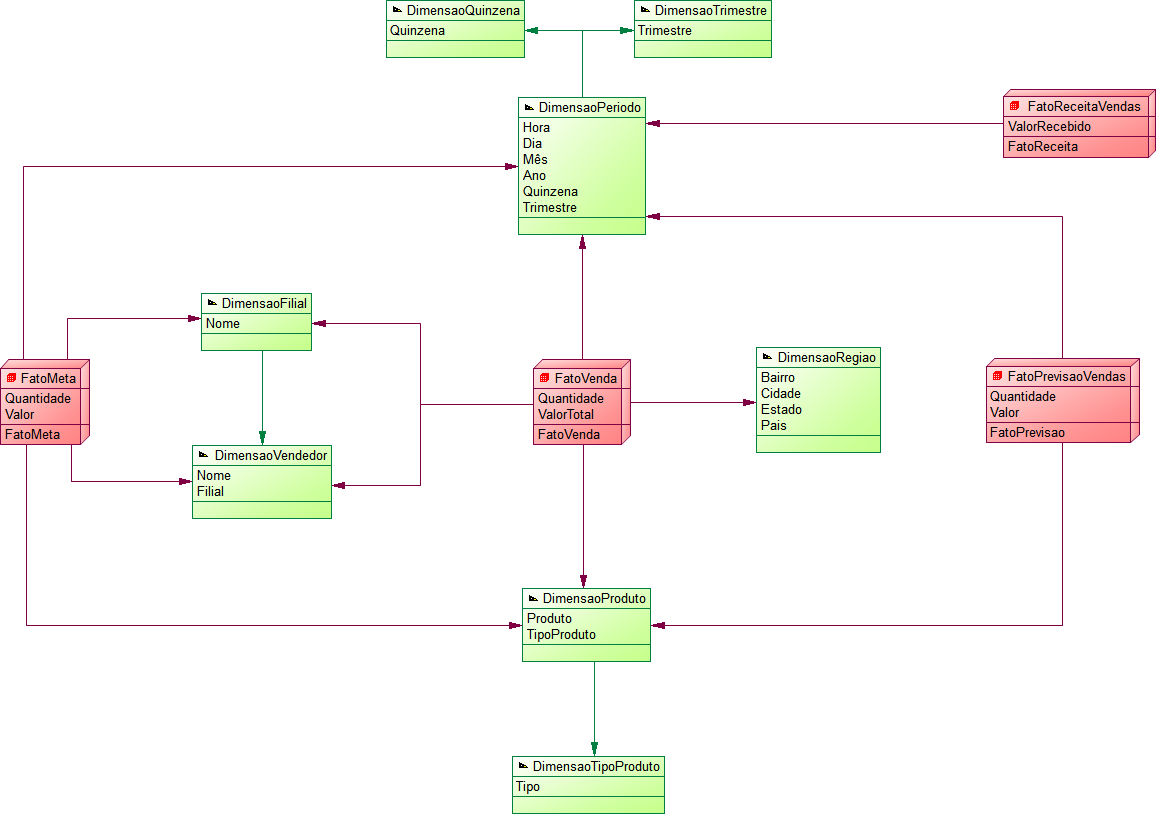
\includegraphics[width=15.997cm,height=11.264cm]{monograph-img017.png} \newline
\newline
\textsf{\MakeUppercase{FIGURA 17}}\textsf{: Modelo Dimensional de Dados. }}

{\selectlanguage{portuges}
\textsf{O modelo dimensional de dados, conforme apresentado na Figura 17, \'e composto por quatro tabelas fato, que
s\~ao FatoVenda, FatoMeta, FatoReceitaVendas e FatoPrevisaoVendas, e oito tabelas dimens\~ao, que s\~ao
DimensaoProduto, DimensaoTipoProduto, DimensaoFilial, DimensaoVendedor, DimensaoPeriodo, DimensaoQuinzena,
DimensaoTrimestre e DimensaoRegiao, descritos a seguir:}}

\liststyleWWviiiNumxvii
\begin{enumerate}
\item {\selectlanguage{portuges}
\textsf{FatoVenda: Tabela fato principal do sistema, que cont\'em as medidas Quantidade, que armazena a quantidade de
itens vendidos, e Valor Total, que representa a soma dos valores dos itens desta venda. FatoVenda tem relacionamento N
x 1 (muitos para um) com as tabelas DimensaoProduto, DimensaoFilial, DimensaoVendedor, DimensaoPeriodo e
DimensaoRegiao, sendo que para cada FatoVenda pode se ter apenas um registro nessas tabelas Dimens\~ao;}}
\item {\selectlanguage{portuges}
\textsf{FatoMeta: Tabela fato auxiliar do sistema, que cont\'em as medidas Quantidade, que armazena a meta de quantidade
de itens vendidos, e Valor Total, que representa a soma dos valores dos itens desta meta. FatoMeta tem relacionamento N
x 1 (muitos para um) com as tabelas DimensaoProduto, }\textsf{DimensaoFilial, DimensaoVendedor e DimensaoPeriodo, sendo
que para cada FatoMeta pode se ter apenas um registro nessas tabelas Dimens\~ao; }}
\item {\selectlanguage{portuges}
\textsf{FatoReceitaVendas: Tabela fato auxiliar do sistema, que cont\'em a medida ValorRecebido, que armazena o valor
recebido em determinado per\'iodo. FatoReceitaVendas tem relacionamento N x 1 (muitos para um) com a tabela
DimensaoPeriodo, sendo que para cada FatoReceitaVendas pode se ter apenas um registro nessa tabela Dimens\~ao;}}
\item {\selectlanguage{portuges}
\textsf{FatoPrevisaoVendas: Tabela fato auxiliar do sistema, que cont\'em as medidas Quantidade, que armazena a
previs\~ao de quantidade de itens vendidos, e Valor Total, que representa a soma dos valores dos itens desta
previs\~ao. FatoPrevisaoVendas tem relacionamento N x 1 (muitos para um) com as tabelas DimensaoProduto e
DimensaoPeriodo, sendo que para cada FatoPrevisaoVendas pode se ter apenas um registro nessas tabelas Dimens\~ao;}}
\item {\selectlanguage{portuges}
\textsf{DimensaoProduto: Dimens\~ao que representa o produto vendido. Possui os atributos Produto, que cont\'em o nome
do produto, e TipoProduto, que cont\'em a chave estrangeira respons\'avel pelo relacionamento N x 1 (muitos para um)
com a tabela DimensaoTipoProduto, onde cada produto s\'o pode ter um tipo. Al\'em da tabela DimensaoTipoProduto, a
tabela DimensaoProduto possui relacionamento com 1 x N (um para muitos) com as tabelas FatoVenda, FatoMeta e
FatoPrevisaoVendas, onde para cada produto podem existir um ou v\'arios registros nas tabelas Fato citadas;}}
\item {\selectlanguage{portuges}
\textsf{DimensaoTipoProduto: Dimens\~ao que representa o tipo de produto vendido. Possui o atributo Tipo, que cont\'em o
nome do tipo de produto. Possui relacionamento 1 x N (um para muitos) com a tabela DimensaoProduto, onde para cada tipo
de produto podem existir um ou v\'arios registros na tabela DimensaoProduto;}}
\item {\selectlanguage{portuges}
\textsf{DimensaoFilial: Dimens\~ao que representa a filial que efetuou a venda. Possui o atributo Nome, que cont\'em o
nome da filial. DimensaoFilial possui relacionamento com 1 x N (um para muitos) com as tabelas FatoVenda, \ FatoMeta, e
DimensaoVendedor, onde para cada filial podem existir um ou v\'arios registros nas tabelas citadas; }}
\item {\selectlanguage{portuges}
\textsf{DimensaoVendedor: Dimens\~ao que representa o vendedor que efetuou a venda. Possui o atributo Nome, que cont\'em
o nome do vendedor, e Filial, que cont\'em a chave estrangeira respons\'avel pelo relacionamento com a tabela
DimensaoFilial, com a qual possui um relacionamento N x 1 (muitos para 1), onde um vendedor s\'o pode pertencer a uma
filial. DimensaoVendedor possui relacionamento com 1 x N (um para muitos) com as tabelas FatoVenda e FatoMeta, onde
para cada vendedor podem existir um ou v\'arios registros nas tabelas citadas; \ }}
\item {\selectlanguage{portuges}
\textsf{DimensaoPeriodo Dimens\~ao que representa a data em que foi efetuada a venda. Possui os atributos Hora, Dia,
M\^es e Ano, que cont\'em os dados referentes \`a data da venda, Quinzena, que cont\'em a chave estrangeira
respons\'avel pelo relacionamento N x 1 (muitos para um) com a tabela DimensaoQuinzena, onde cada registro da tabela
DimensaoPeriodo s\'o pode estar associado a uma quinzena, e o atributo Trimestre, que cont\'em a chave estrangeira
respons\'avel pelo relacionamento N x 1 (muitos para um) com a tabela DimensaoTrimestre, onde cada registro da tabela
DimensaoPeriodo s\'o pode estar associado a um trimestre. Al\'em das tabelas DimensaoQuinzena e DimensaoTrimestre,, a
tabela DimensaoPeriodo possui relacionamento com 1 x N (um para muitos) com as tabelas FatoVenda, FatoMeta,
FatoReceitaVendas e FatoPrevisaoVendas, onde para cada produto podem existir um ou v\'arios registros nas tabelas Fato
citadas;}}
\item {\selectlanguage{portuges}
\textsf{DimensaoQuinzena: Dimens\~ao que representa a quinzena de determinado per\'iodo. Possui o atributo Quinzena, que
representa o n\'umero da quinzena do per\'iodo da venda. DimensaoQuinzena possui relacionamento 1 x N (um para muitos)
com a tabela DimensaoPeriodo, onde para cada quinzena existem um ou v\'arios registros per\'iodos associados;}}
\item {\selectlanguage{portuges}
\textsf{DimensaoTrimestre: Dimens\~ao que representa o trimestre de determinado per\'iodo. Possui o atributo Trimestre,
que representa o n\'umero do trimestre do per\'iodo da venda. DimensaoTrimestre possui relacionamento 1 x N (um para
muitos) com a tabela DimensaoPeriodo, onde para cada trimestre existem um ou v\'arios registros per\'iodos
associados;}}
\item {\selectlanguage{portuges}
\textsf{DimensaoRegiao: Dimens\~ao que representa a regi\~ao do cliente que efetuou determinada compra. Possui os
atributos Bairro, Cidade, Estado e Pa\'is, que cont\'em os dados referentes \`a regi\~ao do cliente. DimensaoRegiao
possui }\textsf{relacionamento 1 x N (um para muitos) com a tabela FatoVenda, onde uma regi\~ao pode possuir uma ou
v\'arias vendas.}}
\end{enumerate}

\bigskip

\liststyleWWviiiNumi
\begin{enumerate}
\item \begin{enumerate}
\item {\selectlanguage{portuges}
\textsf{TECNOLOGIAS UTILIZADAS NA PROTOTIPA\c{C}\~AO}}
\end{enumerate}
\end{enumerate}
{\selectlanguage{portuges}\sffamily
A seguir ser\~ao explanadas as tecnologias utilizadas na arquitetura do projeto do SIG de Vendas da NIB Ferragens.}


\bigskip

\liststyleWWviiiNumi
\setcounter{saveenum}{\value{enumi}}
\begin{enumerate}
\setcounter{enumi}{\value{saveenum}}
\item \setcounter{saveenum}{\value{enumii}}
\begin{enumerate}
\setcounter{enumii}{\value{saveenum}}
\item \setcounter{saveenum}{\value{enumiii}}
\begin{enumerate}
\setcounter{enumiii}{\value{saveenum}}
\item {\selectlanguage{portuges}
\textsf{\textbf{Armazenamento do Data Mart}}}
\end{enumerate}
\end{enumerate}
\end{enumerate}
{\selectlanguage{portuges}
\textsf{Para a cria\c{c}\~ao e armazenamento do }\textsf{\textit{Data Mart}}\textsf{, suas tabelas, otimiza\c{c}\~ao do
desempenho das consultas e armazenamento dos dados foi utilizado o Sistema Gerenciador de Bancos de Dados
}\textsf{\textit{Oracle Database 11g}}\textsf{, pelas seguintes raz\~oes: }}

\liststyleWWviiiNumxiv
\begin{enumerate}
\item {\selectlanguage{portuges}
\textsf{Possui alta confiabilidade, seguran\c{c}a e agilidade;}}
\item {\selectlanguage{portuges}
\textsf{F\'acil de criar e gerenciar bancos de dados de }\textsf{\textit{Data Warehousing}}\textsf{;}}
\item {\selectlanguage{portuges}\sffamily
\'E otimizado para se trabalhar com grandes volumes de dados;}
\item {\selectlanguage{portuges}
\textsf{\'E consolidado no mercado, sendo o sistema gerenciador de banco de dados corporativo mais utilizado do mundo;}}
\item {\selectlanguage{portuges}
\textsf{Possui uma vers\~ao gratuita (}\textsf{\textit{Express Edition}}\textsf{), uma vers\~ao voltada para pequenas e
m\'edias empresas (}\textsf{\textit{Standard Edition}}\textsf{), e uma vers\~ao para grandes corpora\c{c}\~oes
(}\textsf{\textit{Enterprise Edition}}\textsf{), o que reduz os futuros custos de implanta\c{c}\~ao e manuten\c{c}\~ao
de um SIG de Vendas e ir\'a garantir uma alta escalabilidade para o projeto (a vers\~ao utilizada na elabora\c{c}\~ao
deste prot\'otipo, a Express Edition, \'e voltada apenas para fins educacionais, n\~ao podendo ser utilizada em
ambientes de produ\c{c}\~ao);}}
\item {\selectlanguage{portuges}
\textsf{\'E compat\'ivel com mais de 20 plataformas, que incluem }\textsf{\textit{Linux}}\textsf{,
}\textsf{\textit{Windows}}\textsf{, }\textsf{\textit{Mac OS}}\textsf{, }\textsf{\textit{Solaris}}\textsf{,
}\textsf{\textit{HP-UX}}\textsf{ e }\textsf{\textit{IBM AIX}}\textsf{;}}
\item {\selectlanguage{portuges}\sffamily
Oferece uma extensa gama de softwares certificados, suporte, treinamento e consultoria.}
\end{enumerate}

\bigskip


\bigskip

\liststyleWWviiiNumi
\begin{enumerate}
\item \begin{enumerate}
\item \begin{enumerate}
\item {\selectlanguage{portuges}
\textsf{\textbf{Camada de ETL}}}
\end{enumerate}
\end{enumerate}
\end{enumerate}
{\selectlanguage{portuges}
\textsf{Para a realiza\c{c}\~ao das tarefas de extra\c{c}\~ao, transforma\c{c}\~ao e carga, integrando o sistema de
gerenciamento de banco de dados dos sistemas de processamento de transa\c{c}\~oes da NIB Ferragens ao
}\textsf{\textit{Oracle Database 11g}}\textsf{, foi utilizada a ferramenta }\textsf{\textit{Pentaho Data
Integration}}\textsf{, escolhida pelas seguintes raz\~oes:}}

\liststyleWWviiiNumxxx
\begin{enumerate}
\item {\selectlanguage{portuges}
\textsf{Larga conectividade com qualquer tipo de dado, incluindo grandes volumes de dados;}}
\item {\selectlanguage{portuges}
\textsf{Suporte a m\'ultiplas fontes de dados, dentre elas, os principais sistemas de gerenciamento de bancos de dados
do mercado e os tipos de arquivo e softwares de escrit\'orio mais utilizados;}}
\item {\selectlanguage{portuges}\sffamily
Escalabilidade e desempenho corporativos;}
\item {\selectlanguage{portuges}
\textsf{Ferramentas gr\'aficas avan\c{c}adas que permitem a usu\'arios n\~ao desenvolvedores f\'acil utiliza\c{c}\~ao na
integra\c{c}\~ao de novas fontes de dados, sem a necessidade da cria\c{c}\~ao de c\'odigos;}}
\item {\selectlanguage{portuges}\sffamily
Ferramentas gr\'aficas que permitem a cria\c{c}\~ao de mapas de dados possibilitando inclusive transforma\c{c}\~oes
complexas entre os dados das fontes e do destino;}
\item {\selectlanguage{portuges}
\textsf{\'E um software que possui uma vers\~ao gratuita, ideal para a fase de implanta\c{c}\~ao e in\'icio da
utiliza\c{c}\~ao do projeto, sendo que esta deve ser migrada para a vers\~ao comercial assim que o projeto entrar em
ambiente de produ\c{c}\~ao;}}
\item {\selectlanguage{portuges}
\textsf{\'E compat\'ivel com os principais sistemas operacionais do mercado. }}
\end{enumerate}

\bigskip

\liststyleWWviiiNumi
\begin{enumerate}
\item \begin{enumerate}
\item \begin{enumerate}
\item {\selectlanguage{portuges}
\textsf{\textbf{Mapeamento do Modelo Dimensional e da Camada Visual}}}
\end{enumerate}
\end{enumerate}
\end{enumerate}
{\selectlanguage{portuges}
\textsf{A camada visual do sistema foi elaborada utilizando-se a plataforma de BI da MicroStrategy, que, segundo
Hagerty, Sallam e Richardson (2012, p. 18), est\'a posicionada como plataforma l\'ider em BI no mercado. A plataforma
de BI da MicroStrategy possibilita an\'alises profundas e em tempo real com interfaces interativas e funcionalidades
anal\'iticas para uso por um grande volume de usu\'arios por meio de navegadores Web, dispositivos m\'oveis e
aplicativos Office.}}

{\selectlanguage{portuges}\sffamily
A escolha da plataforma de BI da MicroStrategy como camada visual do sistema foi feita levando-se em conta os seguintes
aspectos:}

\liststyleWWviiiNumxxi
\begin{enumerate}
\item {\selectlanguage{portuges}
\textsf{Modelo multidimensional blindado, o qual garante que informa\c{c}\~oes cr\'iticas permane\c{c}am seguras;}}
\item {\selectlanguage{portuges}
\textsf{Permite que os aplicativos criados na plataforma sejam escal\'aveis e se adaptem \`a evolu\c{c}\~ao nas cargas
dos usu\'arios e nos requisitos em desenvolvimento;}}
\item {\selectlanguage{portuges}
\textsf{Possui um abrangente conjunto de produtos que reduzem as despesas administrativas dos aplicativos de BI;}}
\item {\selectlanguage{portuges}
\textsf{Proporciona, segundo Hagerty, Sallam e Richardson (2012, p. 18), a interface mais intuitiva e f\'acil de usar
dentre as plataformas de BI do mercado;}}
\item {\selectlanguage{portuges}
\textsf{Unifica\c{c}\~ao e reutiliza\c{c}\~ao dos metadados, fornecendo uma plataforma de metadados orientada a objetos,
que define a camada de neg\'ocios corporativa em um \'unico reposit\'orio compartilhada;}}
\item {\selectlanguage{portuges}\sffamily
Plataforma de interface independente, que permite ao usu\'ario acessar e analisar suas informa\c{c}\~oes em dispositivos
m\'oveis, navegadores web ou aplicativos Microsoft Office.}
\end{enumerate}

\bigskip

\liststyleWWviiiNumi
\begin{enumerate}
\item \begin{enumerate}
\item \begin{enumerate}
\item {\selectlanguage{portuges}
\textsf{\textbf{Camada de Servidor}}}
\end{enumerate}
\end{enumerate}
\end{enumerate}
{\selectlanguage{portuges}
\textsf{O }\textsf{\textit{Windows Server 2008}}\textsf{, da Microsoft, foi selecionado como sistema operacional para
abrigar o servidor OLAP do sistema. Ele prov\^e maior ader\^encia \`a plataforma de BI da MicroStrategy, uma vez que,
segundo a documenta\c{c}\~ao da MicroStrategy (2011, p. 38-41), alguns produtos apenas funcionam no sistema operacional
}\textsf{\textit{Windows}}\textsf{, como o }\textsf{\textit{MicroStrategy Architect}}\textsf{ e o
}\textsf{\textit{MicroStrategy Desktop}}\textsf{, sendo que produtos como o }\textsf{\textit{MicroStrategy Intelligence
Server}}\textsf{ est\~ao certificados apenas para vers\~oes especificamente criadas para servidores, como o
}\textsf{\textit{Windows Server 2003}}\textsf{ e o }\textsf{\textit{Windows Server 2008}}\textsf{, caso o
}\textsf{\textit{Windows}}\textsf{ seja escolhido como sistema operacional.}}

{\selectlanguage{portuges}
\textsf{A escolha do }\textsf{\textit{Windows Server 2008}}\textsf{ como sistema operacional do projeto do SIG de Vendas
da NIB Ferragens ocorreu devido aos seguintes aspectos:}}

\liststyleWWviiiNumxiii
\begin{enumerate}
\item {\selectlanguage{portuges}
\textsf{O Windows Server 2008 \'e o sistema operacional da plataforma Windows Server mais seguro j\'a criado;}}
\item {\selectlanguage{portuges}
\textsf{Possui a vers\~ao 7.0 do Internet Information Services, que possibilita maior ader\^encia ao ASP.Net, ambiente
padr\~ao dos servidores Web da plataforma de BI da MicroStrategy;}}
\item {\selectlanguage{portuges}
\textsf{Possui uma base s\'olida para cargas de trabalho corporativas, sendo o mais robusto e flex\'ivel sistema
operacional Windows Server para dados. }}
\end{enumerate}

\bigskip

\liststyleWWviiiNumi
\begin{enumerate}
\item \begin{enumerate}
\item \begin{enumerate}
\item {\selectlanguage{portuges}
\textsf{\textbf{Plataforma M\'ovel -- Camada de Acesso \`as Informa\c{c}\~oes}}}
\end{enumerate}
\end{enumerate}
\end{enumerate}
{\selectlanguage{portuges}
\textsf{O }\textsf{\textit{Android 4.0}}\textsf{, da Google, foi selecionado como sistema operacional m\'ovel para se
efetuar a implementa\c{c}\~ao da camada visual do projeto. A Google disponibiliza de forma gratuita um emulador que
permite que sejam realizados testes de visualiza\c{c}\~ao sem que se precise um dispositivo m\'ovel f\'isico. O sistema
operacional }\textsf{\textit{iOS}}\textsf{, da Apple, tamb\'em poderia ser selecionado como sistema operacional m\'ovel
para a camada visual do projeto, por\'em, o Android possui uma grande variedade de tablets de diferentes pre\c{c}os e
fabricantes, trazendo maior flexibilidade, enquanto o iOS s\'o \'e encontrado nos tablets da Apple, os iPads que, em
geral, s\~ao produtos com pre\c{c}os mais elevados. }}


\bigskip

\liststyleWWviiiNumi
\setcounter{saveenum}{\value{enumi}}
\begin{enumerate}
\setcounter{enumi}{\value{saveenum}}
\item \setcounter{saveenum}{\value{enumii}}
\begin{enumerate}
\setcounter{enumii}{\value{saveenum}}
\item {\selectlanguage{portuges}\sffamily
RESTRI\c{C}\~OES DE IMPLEMENTA\c{C}\~AO}
\end{enumerate}
\end{enumerate}
{\sffamily
Considerando o escopo deste trabalho, foram estabelecidas algumas restri\c{c}\~oes de
\foreignlanguage{portuges}{implementa\c{c}\~ao para o prot\'otipo, as quais foram consideradas como essenciais as que
se referem aos seguintes casos de uso:}}

\liststyleWWviiiNumx
\begin{enumerate}
\item {\selectlanguage{portuges}
\textsf{ConsultaVendasRealizadasPrevistasPeriodo;}}
\item {\selectlanguage{portuges}
\textsf{ConsultaDemonstrativoVendasUltimos15Dias;}}
\item {\selectlanguage{portuges}
\textsf{ConsultaVendasMetas;}}
\item {\selectlanguage{portuges}
\textsf{ConsultaVendedorVendasMetas;}}
\item {\selectlanguage{portuges}
\textsf{ConsultaTipoProdutoVendasMetas;}}
\item {\selectlanguage{portuges}
\textsf{ConsultaFilialVendasMetas.}}
\end{enumerate}
{\selectlanguage{portuges}\sffamily
A implementa\c{c}\~ao deste trabalho estar\'a restrita \`a execu\c{c}\~ao do sistema por parte do Gerente Geral de
Vendas, excluindo-se do escopo deste trabalho a cria\c{c}\~ao de interfaces para os Gerentes das Filiais e para os
Vendedores.}

{\selectlanguage{portuges}
\textsf{Os dados utilizados na implementa\c{c}\~ao deste trabalho s\~ao fict\'icios, bem como n\~ao correspondem ao
escopo deste trabalho as especifica\c{c}\~oes de metas e previs\~oes, sendo estas tamb\'em meramente ilustrativas e
fict\'icias.}}


\bigskip

\liststyleWWviiiNumi
\begin{enumerate}
\item \begin{enumerate}
\item {\selectlanguage{portuges}\sffamily
FLUXO DE EXECU\c{C}\~AO }
\end{enumerate}
\end{enumerate}
{\selectlanguage{portuges}
\textsf{A Figura 18 representa o fluxo de execu\c{c}\~ao do SIG M\'ovel de Vendas da NIB Ferragens, a ser explanado a
seguir.}}

\newline
 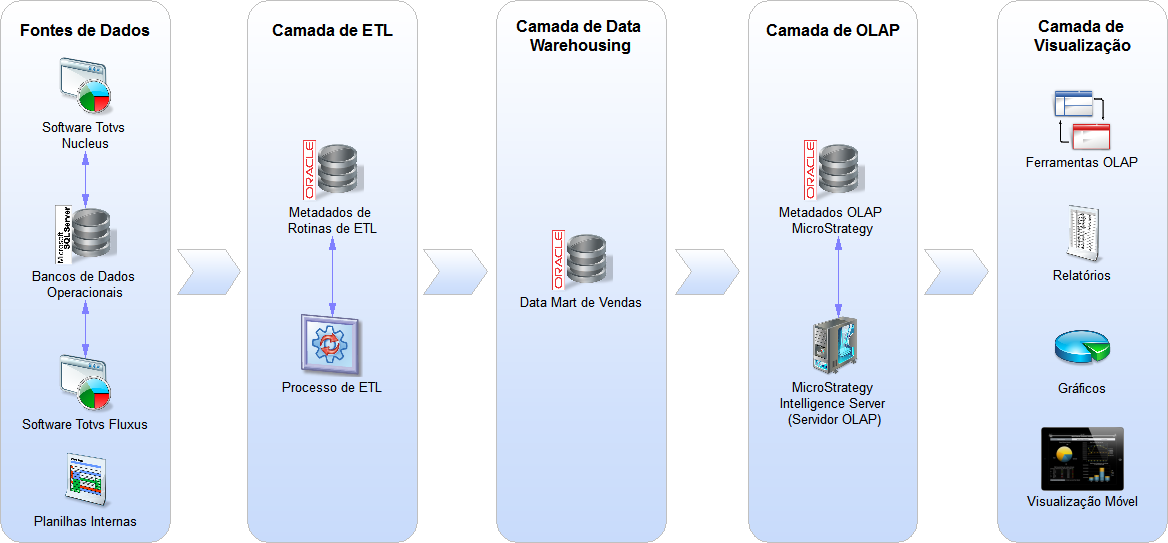
\includegraphics[width=15.977cm,height=7.428cm]{monograph-img018.png} 

{\selectlanguage{portuges}
\textsf{\MakeUppercase{FIGURA 18}}\textsf{: Fluxo de execu\c{c}\~ao do sistema.\newline
}}

{\selectlanguage{portuges}
\textsf{Conforme apresentado no cap\'itulo 2, o fluxo de execu\c{c}\~ao do Sistema de Informa\c{c}\~oes Gerenciais
M\'ovel de Vendas da NIB Ferragens pode ser dividido em cinco camadas:}}

\liststyleWWviiiNumxix
\begin{enumerate}
\item {\selectlanguage{portuges}
\textsf{Camada de Fontes de Dados, que contemplam os dados dos bancos de dados operacionais, alimentados pelos softwares
transacionais Totvs Nucleus e Totvs Fluxus, e dados extra\'idos de planilhas de controle de vendas internas;}}
\item {\selectlanguage{portuges}
\textsf{Camada de ETL, que contempla a execu\c{c}\~ao e armazenamento das rotinas de ETL do sistema, onde os dados s\~ao
extra\'idos da camada de Fontes de Dados, transformados e carregados na camada de Data Warehousing. Nesta camada, foi
modelado no software Pentaho Data Integration todo o processamento ETL que, para este prot\'otipo, consta da
cria\c{c}\~ao do mapeamento das colunas nas tabelas fonte dos bancos de dados dos sistemas Totvs Nucleus e Totvs
Fluxus, elabora\c{c}\~ao dos passos de transforma\c{c}\~ao e formata\c{c}\~ao destes dados para a carga em todas as
tabelas fato e dimens\~ao do Modelo Dimensional apresentado na se\c{c}\~ao 4.1;}}
\item {\selectlanguage{portuges}
\textsf{Camada de Data Warehousing, que contempla o armazenamento dos dados transformados pela camada de ETL num banco
de dados multidimensional espec\'ifico para a \'area de vendas, o Data Mart de Vendas. Esta camada utiliza o Oracle
Database 11g, armazena o Data Mart criado de acordo com o Modelo Dimensional apresentado na se\c{c}\~ao 4.1 e recebe a
carga dos dados transformados pelo processo de ETL;}}
\item {\selectlanguage{portuges}
\textsf{Camada de OLAP, que contempla o mapeamento do Data Mart de Vendas no ambiente de OLAP do MicroStrategy
Intelligence Server e o armazenamento dos metadados de mapeamento. Para este mapeamento \'e necess\'ario que o Modelo
Dimensional esteja projetado e modelado corretamente, uma vez que \'e necess\'ario mapear no MicroStrategy Intelligence
Server quais colunas de cada tabela representam os Fatos e Atributos (denomina\c{c}\~ao dada pela MicroStrategy \`as
dimens\~oes), mapear os relacionamentos entre os fatos e atributos, para que s\'o a partir disto as an\'alises OLAP
funcionem. As an\'alises OLAP do MicroStrategy s\~ao sens\'iveis \`a boa elabora\c{c}\~ao do modelo, e ao menor
equ\'ivoco no mapeamento ou na elabora\c{c}\~ao do projeto ir\'a exibir dados n\~ao conformes ou n\~ao ir\'a gerar os
relat\'orios das an\'alises. A partir do correto mapeamento, nesta camada que \'e criada a camada de visualiza\c{c}\~ao
do sistema de BI, onde \'e modelado cada relat\'orio, criado e formatado os gr\'aficos, formatada cada
visualiza\c{c}\~ao de determinado ator e elaboradas as poss\'iveis intera\c{c}\~oes do usu\'ario com o sistema. Nesta
camada tamb\'em que se \'e poss\'ivel a formata\c{c}\~ao }\textsf{espec\'ifica para determinada plataforma, e no caso
desta proposta, foi elaborada a visualiza\c{c}\~ao espec\'ifica para o Android como plataforma m\'ovel, onde s\~ao
especificados comportamentos espec\'ificos que determinados recursos e controles visuais devem executar, entre
outros;}}
\item {\selectlanguage{portuges}
\textsf{Camada de Visualiza\c{c}\~ao, que contempla as ferramentas visuais de OLAP, os Relat\'orios, os Gr\'aficos e a
Visualiza\c{c}\~ao em ambiente M\'ovel. Para este prot\'otipo, o Android foi selecionado como plataforma m\'ovel, ao
qual a MicroStrategy possui uma aplica\c{c}\~ao cliente que acessa os gr\'aficos, relat\'orios e visualiza\c{c}\~oes
criados no software MicroStrategy (Camada de OLAP), capta as requisi\c{c}\~oes de recursos e comportamentos
espec\'ificos e os traduz para o formato de aplica\c{c}\~ao nativa do Android, tornando a intera\c{c}\~ao com o sistema
de BI amig\'avel e com r\'apidas respostas. O usu\'ario ainda pode interagir com filtros e sele\c{c}\~oes previamente
criadas para os relat\'orios e gr\'aficos criados por meio de controles e pesquisas espec\'ificas do Android.}}
\end{enumerate}

\bigskip

\liststyleWWviiiNumi
\begin{enumerate}
\item \begin{enumerate}
\item {\selectlanguage{portuges}\sffamily
ARQUITETURA DO SISTEMA }
\end{enumerate}
\end{enumerate}
{\selectlanguage{portuges}
\textsf{A Figura 19 representa a arquitetura do sistema, a qual \'e composta pela infra-estrutura de inform\c{c}\~oes
que consta na matriz e a distribui\c{c}\~ao destas informa\c{c}\~oes via internet aos Tablets dos usu\'arios do
sistema. Na base da arquitetura do sistema tem-se o servidor do Banco de Dados dos SPTs da NIB, que \'e acessado pelo
Servidor de ETL, que, ap\'os efetuar o processamento e transforma\c{c}\~ao destes dados, os carrega no Data Mart
inclu\'ido no Servidor de Data Warehousing. No topo da infraestrutura projetada para o sistema est\'a o Servidor OLAP,
que, por meio do software MicroStrategy Intelligence Server, fornece a interface de transfer\^encia de metadados e
informa\c{c}\~oes que ser\~ao acessados e visualizados nos tablets Android por meio da Internet, em qualquer lugar que
os usu\'arios portadores destes tablets estejam localizados que possua algum tipo de conex\~ao com a Internet. }}

 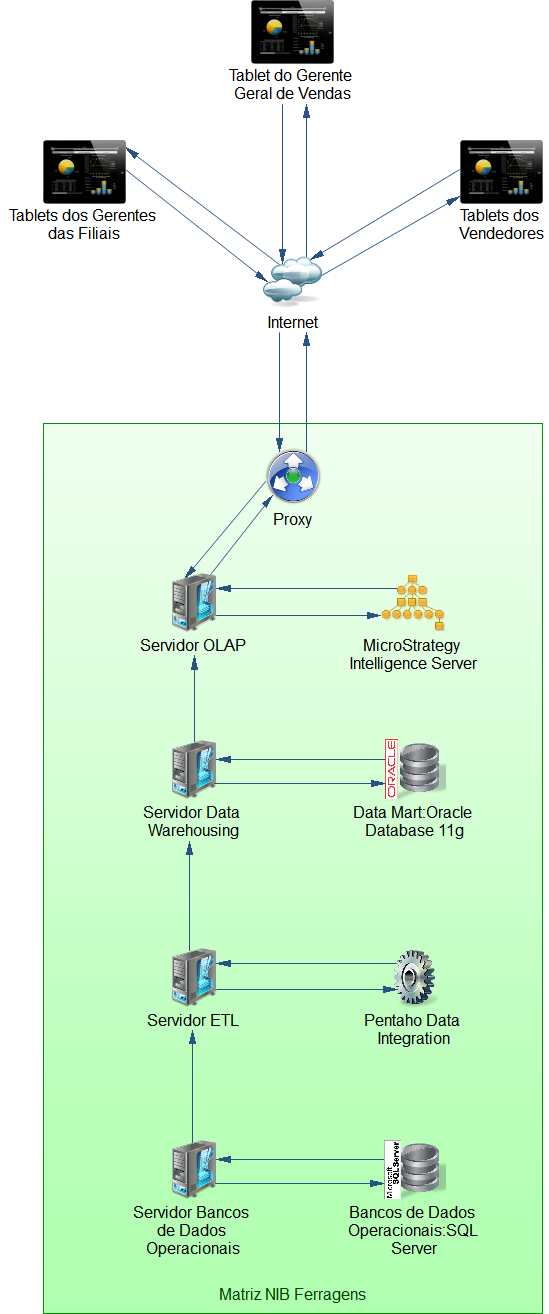
\includegraphics[width=9.617cm,height=22.983cm]{monograph-img019.png} 

{\selectlanguage{portuges}
\textsf{\MakeUppercase{FIGURA 19}}\textsf{: Arquitetura do sistema.}}

\liststyleWWviiiNumi
\setcounter{saveenum}{\value{enumi}}
\begin{enumerate}
\setcounter{enumi}{\value{saveenum}}
\item \setcounter{saveenum}{\value{enumii}}
\begin{enumerate}
\setcounter{enumii}{\value{saveenum}}
\item {\selectlanguage{portuges}\sffamily
PROT\'OTIPO DO SISTEMA}
\end{enumerate}
\end{enumerate}
{\selectlanguage{portuges}
\textsf{A seguir ser\~ao disponibilizadas as telas do prot\'otipo desenvolvido de acordo com as restri\c{c}\~oes
apresentadas na se\c{c}\~ao 4.3 deste trabalho.}}

{\selectlanguage{portuges}
\textsf{A Figura 20 apresenta a tela inicial do sistema onde s\~ao disponibilizadas as informa\c{c}\~oes referentes aos
principais resultados das vendas da NIB Ferragens dos \'ultimos 15 dias. As seguintes vis\~oes est\~ao dispon\'iveis
nesta tela:}}

\liststyleWWviiiNumxx
\begin{enumerate}
\item {\selectlanguage{portuges}
\textsf{Total de Vendas por Filial -- \'Ultimos 15 Dias: \'E representado por meio de um gr\'afico de Pizza, o qual \'e
dividido entre as filiais e seus resultados em volumes de vendas. Cada filial \'e representada por uma fatia de
determinada cor. Ao se clicar em determinada fatia do gr\'afico, \'e exibido o desempenho da determinada filial
clicada;}}
\item {\selectlanguage{portuges}
\textsf{Vendas Realizadas x Vendas Previstas -- \'Ultimos 15 Dias: \'E representado por meio de um gr\'afico de Linhas
que demonstra o volume total de vendas da empresa nos \'ultimos 15 dias comparado \`a previs\~ao de vendas para o mesmo
per\'iodo;}}
\item {\selectlanguage{portuges}
\textsf{Lista de Produtos mais Vendidos nos \'Ultimos 15 Dias: \'E representado por um Quadro, com as colunas Produto,
Quantidade, Meta e Valor, sendo que ao se clicar no t\'itulo da coluna Meta \'e poss\'ivel alternar com a coluna
Previs\~ao;}}
\item {\selectlanguage{portuges}
\textsf{Produtos Mais Vendidos por Filial -- \'Ultimos 15 Dias: \'E representado por um gr\'afico de Colunas compostas,
onde cada coluna representa um produto, dentre os 8 produtos mais vendidos neste per\'iodo. Em cada coluna s\~ao
representadas, por meio de cores, as filiais que compuseram toda a venda daquele determinado produto.}}
\end{enumerate}
 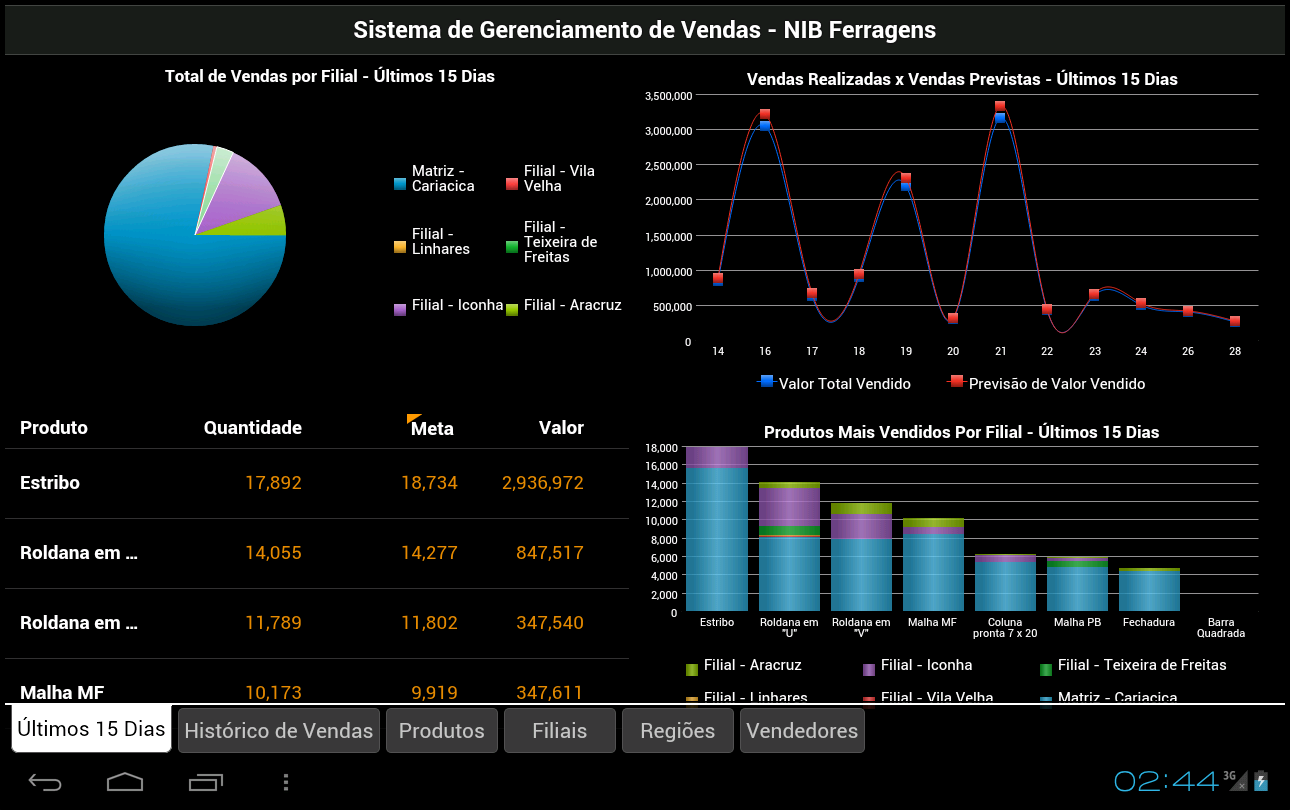
\includegraphics[width=15.968cm,height=10.026cm]{monograph-img020.png} 

{\selectlanguage{portuges}
\textsf{\MakeUppercase{FIGURA 20}}\textsf{: Tela inicial do sistema. }}

{\selectlanguage{portuges}
\textsf{A Figura 21 apresenta a tela com o Hist\'orico de Vendas anual de toda a empresa ou filtrado por filial, onde
s\~ao disponibilizadas as informa\c{c}\~oes referentes aos principais resultados das vendas da NIB Ferragens para cada
m\^es. Inicialmente s\~ao exibidas as informa\c{c}\~oes referentes ao ano corrente e basta ``arrastar'' a tela da
esquerda para a direita que as vis\~oes s\~ao convertidas para o ano anterior, e vice-versa. As seguintes vis\~oes
est\~ao dispon\'iveis nesta tela:}}

\liststyleWWviiiNumxxxii
\begin{enumerate}
\item {\selectlanguage{portuges}
\textsf{Hist\'orico de Vendas por Filial - Anual: \'E representado por meio de um gr\'afico de Linhas, ao qual cada
linha representa uma filial e \'e ilustrado o volume de vendas para cada filial em determinado m\^es do ano;}}
\item {\selectlanguage{portuges}\sffamily
Detalhamento do Volume de Vendas Mensal -- \'E representado por um quadro com a lista de filiais, com as colunas M\^es,
Meta, Previs\~ao e Total em Vendas.}
\end{enumerate}
 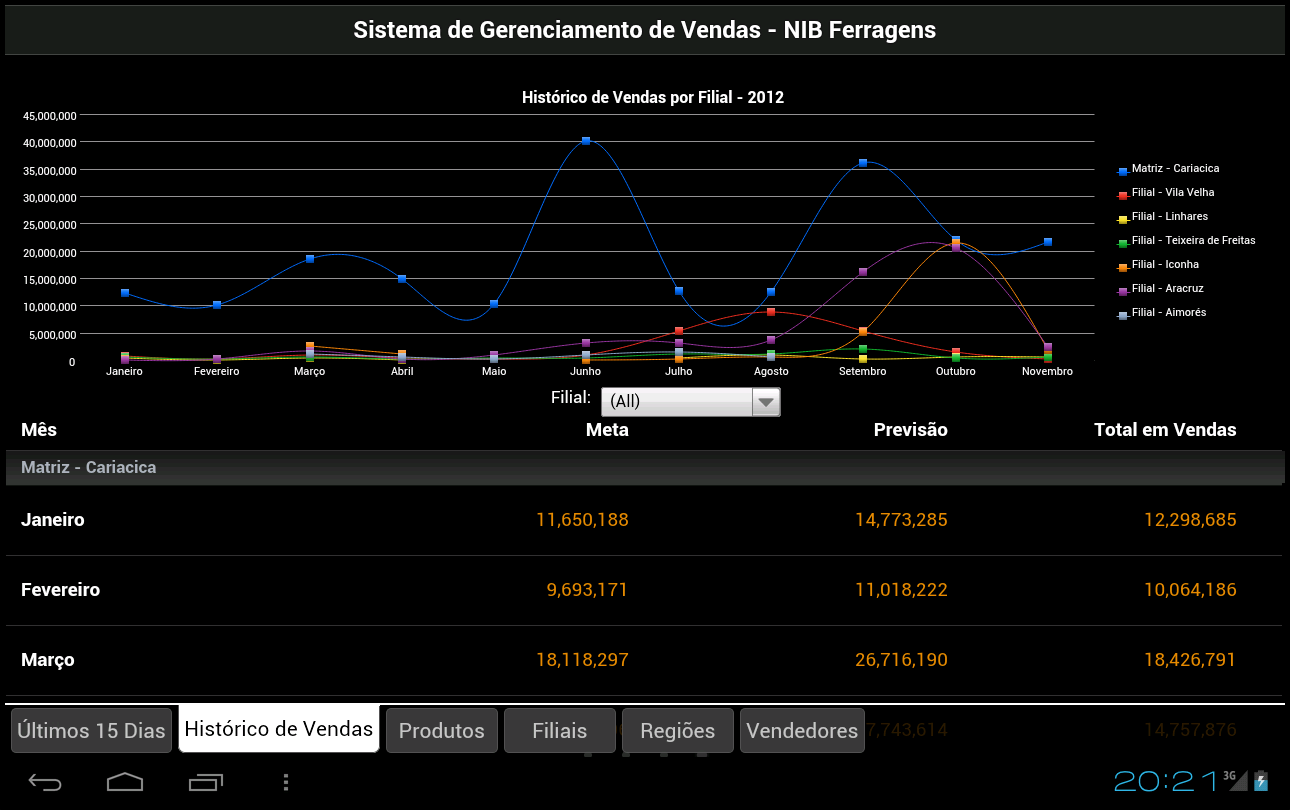
\includegraphics[width=15.976cm,height=10.031cm]{monograph-img021.png} 

{\selectlanguage{portuges}
\textsf{\MakeUppercase{FIGURA 21}}\textsf{: Tela do Hist\'orico de Vendas. }}

{\selectlanguage{portuges}
\textsf{A Figura 22 apresenta a tela com as vendas dos Produtos, onde s\~ao apresentados os desempenhos para cada
produto em determinado ano, seu hist\'orico naquele ano e qual filial apresentou melhor resultado de vendas para ele.
Inicialmente s\~ao exibidas as informa\c{c}\~oes referentes ao ano corrente e basta ``arrastar'' a tela da esquerda
para a direita que as vis\~oes s\~ao convertidas para o ano anterior, e vice-versa. As seguintes vis\~oes est\~ao
dispon\'iveis nesta tela:}}

\liststyleWWviiiNumxxxvii
\begin{enumerate}
\item {\selectlanguage{portuges}
\textsf{Lista de Vendas de Produtos: \'E representado por meio de um Quadro com a lista de produtos na primeira coluna e
a segunda coluna \'e representada, inicialmente, pela Meta, onde \'e exibida a porcentagem de alcance da meta, sendo na
colora\c{c}\~ao verde no caso de supera\c{c}\~ao da meta, vermelho quando a meta n\~ao for alcan\c{c}ada e cinza caso o
desempenho de vendas esteja igualado \`a meta. Esta coluna de metas, ao ser clicado em seu t\'itulo, pode ser alternada
com a Previs\~ao, onde \'e exibida a porcentagem de alcance da previs\~ao, seguindo o mesmo padr\~ao da meta, e a
coluna Vendas, onde \'e exibida a quantidade total de itens vendidos para aquele produto, onde a colora\c{c}\~ao de
cada linha segue o padr\~ao do alcance da meta. Ao se clicar em determinado produto, as vis\~oes da coluna da direita
s\~ao direcionadas a este produto;}}
\item {\selectlanguage{portuges}
\textsf{Hist\'orico de Produtos -- Anual: \'E representado por meio de um gr\'afico de Linhas, ao qual as linhas
representam a Quantidade Vendida (linha azul), a Previs\~ao de Quantidade Vendida (linha vermelha) e a Meta de
Quantidade Vendida (linha amarela), e \'e ilustrado o volume de vendas do produto selecionado para cada m\^es do ano
selecionado, comparado \`a meta e \`a previs\~ao determinadas;}}
\item {\selectlanguage{portuges}\sffamily
Vendas por Filial -- Anual: \'E representado por meio de um gr\'afico de Colunas Horizontais, onde demonstra o
desempenho de vendas das filiais para o produto selecionado.}
\end{enumerate}
 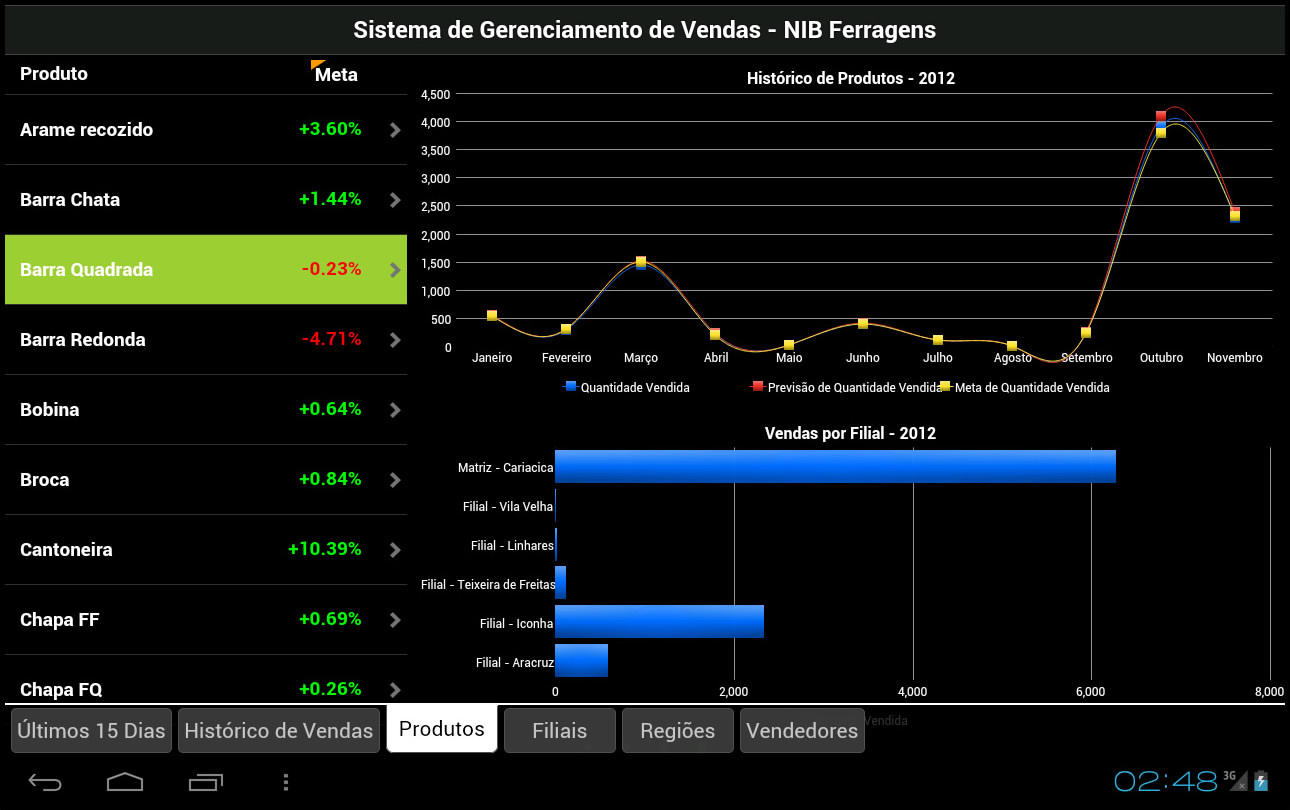
\includegraphics[width=15.972cm,height=10.029cm]{monograph-img022.jpg} 

{\selectlanguage{portuges}
\textsf{\MakeUppercase{FIGURA 22}}\textsf{: Tela de Produtos. }}

{\selectlanguage{portuges}
\textsf{A Figura 23 apresenta a tela com o resultado geral de vendas para cada Localidade, ilustrado por meio de Bolhas
associadas no mapa \`a determinada regi\~ao. O tamanho de cada bolha representa o volume de produtos vendidos de
determinada regi\~ao e as cores representam faixas 4 faixas de vendas, sendo estas:}}

\liststyleWWviiiNumxxxv
\begin{enumerate}
\item {\selectlanguage{portuges}\sffamily
Azul: Acima de 100.000 produtos vendidos;}
\item {\selectlanguage{portuges}\sffamily
Verde: Entre 10.000 e 99.999 produtos vendidos;}
\item {\selectlanguage{portuges}\sffamily
Amarelo: Entre 1.000 e 9.999 produtos vendidos;}
\item {\selectlanguage{portuges}\sffamily
Vermelho: Abaixo de 1.000 produtos vendidos. }
\end{enumerate}
 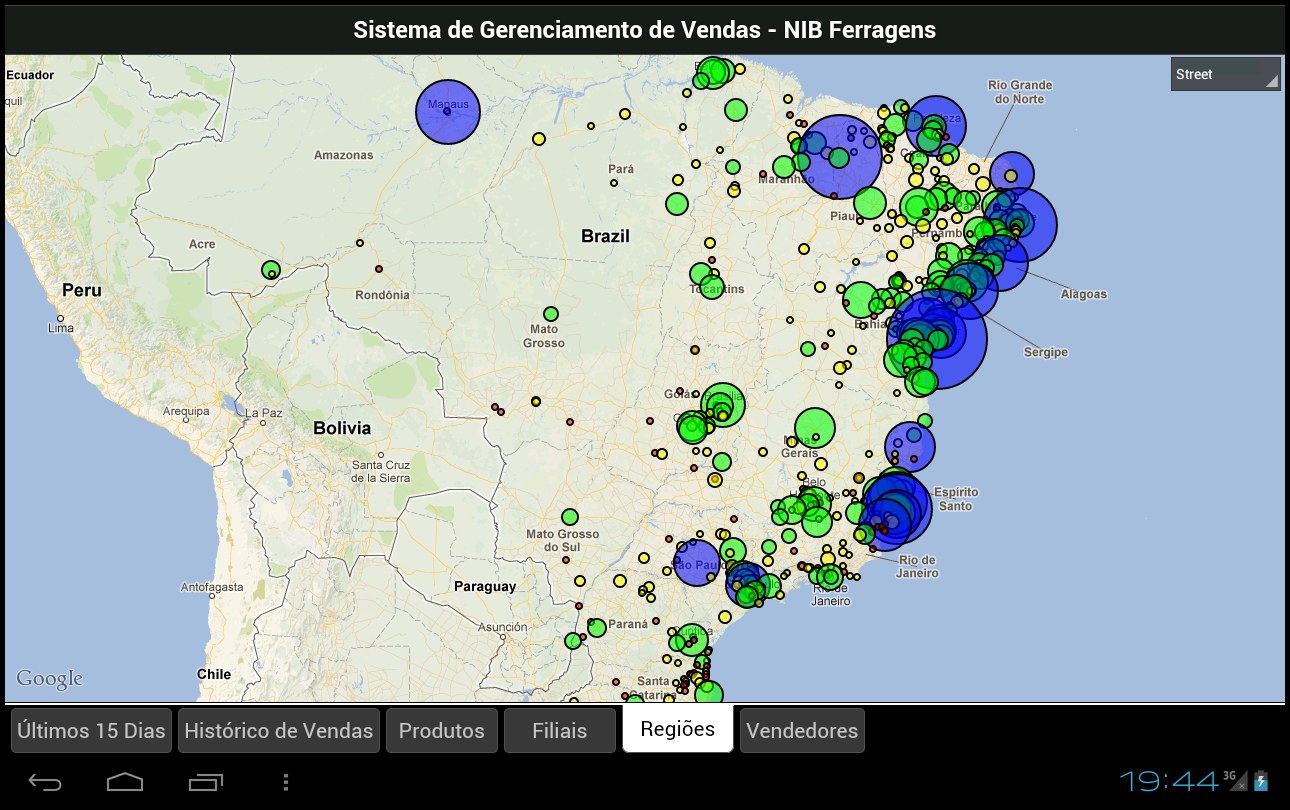
\includegraphics[width=15.976cm,height=10.031cm]{monograph-img023.png} 

{\selectlanguage{portuges}
\textsf{\MakeUppercase{FIGURA 23}}\textsf{: Tela de Regi\~oes. }}


\bigskip

\liststyleWWviiiNumi
\begin{enumerate}
\item \clearpage{\selectlanguage{portuges}\sffamily\bfseries
CONCLUS\~OES E PERSPECTIVAS FUTURAS}
\end{enumerate}

\bigskip

{\selectlanguage{portuges}
\textsf{A demanda apresentada pelo gerente geral de vendas da NIB Ferragens exp\~oe uma defici\^encia potencialmente
comum a outras empresas do ramo de com\'ercio de ferragens, que tamb\'em utilizem como base de sua opera\c{c}\~ao os
sistemas de processamento de transa\c{c}\~oes, com a exist\^encia nula ou deficiente de demonstrativos de resultados
\'ageis e espec\'ificos para o seu ramo de neg\'ocio.}}

{\selectlanguage{portuges}
\textsf{A partir da defini\c{c}\~ao e especifica\c{c}\~ao das necessidades cotidianas da gest\~ao de vendas da NIB
Ferragens foi poss\'ivel formular uma proposta de solu\c{c}\~ao para as mesmas, com foco sempre na
disponibiliza\c{c}\~ao imediata de informa\c{c}\~oes referentes ao centro do neg\'ocio, informa\c{c}\~oes estas que o
gerente de vendas n\~ao disp\~oe por meios autom\'aticos e, no caso de demandas de demonstrativos mais sens\'iveis pela
alta ger\^encia da empresa, os mesmos tem de ser elaborados pela cria\c{c}\~ao manual de planilhas e relat\'orios.}}

{\selectlanguage{portuges}
\textsf{A ado\c{c}\~ao das ferramentas e t\'ecnicas de Intelig\^encia de Neg\'ocios como base para a elabora\c{c}\~ao da
proposta de solu\c{c}\~ao foi a melhor alternativa encontrada dada a heterogeneidade das fontes de dados existentes na
estrutura atual da empresa. Esta op\c{c}\~ao mostrou-se eficiente do ponto de vista da coleta, transforma\c{c}\~ao e
exposi\c{c}\~ao das informa\c{c}\~oes para o gerente de vendas, uma vez que isola os dados de onde s\~ao extra\'idas
estas informa\c{c}\~oes num local externo ao utilizado pelos sistemas de processamento de transa\c{c}\~oes, diminuindo
o tempo de resposta das solicita\c{c}\~oes e gerando os demonstrativos de resultado de forma imediata.}}

{\selectlanguage{portuges}
\textsf{O SIG de Gest\~ao de Vendas M\'ovel possui total abertura a novas implementa\c{c}\~oes que possam vir de acordo
com a demanda da ger\^encia de vendas da empresa. Novos relat\'orios ou demonstrativos podem ser criados a partir das
informa\c{c}\~oes j\'a dispon\'iveis no banco de dados do SIG ou mesmo novas informa\c{c}\~oes podem ser integradas a
este para atendimento de novas demandas. Por meio da utiliza\c{c}\~ao do sistema }\textsf{\textit{Pentaho Data
Integration}}\textsf{, de extra\c{c}\~ao, transforma\c{c}\~ao e carga dos dados das fontes para o banco de dados do SIG
de Gest\~ao de Vendas M\'ovel, \'e poss\'ivel incluir novas fontes de dados de diversas origens, desde arquivos de
planilhas at\'e e-mails e novos sistemas gerenciadores de bancos de dados, dando maior }\textsf{flexibilidade ao
gerente de vendas e enriquecendo a informa\c{c}\~ao gerada pelo sistema.}}

{\selectlanguage{portuges}
\textsf{Como a constru\c{c}\~ao civil no pa\'is \'e um dos setores que mais cresce, o n\'umero de empresas de com\'ercio
de ferragens est\'a crescendo juntamente com o crescimento das empresas j\'a solidificadas no mercado, como a NIB
Ferragens. Seguindo esta premissa do crescimento na ind\'ustria da constru\c{c}\~ao civil, o SIG de Gest\~ao de Vendas
M\'ovel para empresas de com\'ercio de ferragens pode auxiliar a NIB Ferragens a alcan\c{c}ar um bom volume de clientes
a m\'edio prazo e, tendo como base sua mobilidade, agilidade e facilidade de uso, torna-se mais um atrativo aos
gestores de vendas que poder\~ao, a partir dos demonstrativos de desempenho gerados pelo sistema, criar planejamentos e
estrat\'egias espec\'ificas para alcan\c{c}ar um aumento efetivo em seu faturamento e, consequentemente, gerar
crescimento para sua empresa.}}

{\selectlanguage{portuges}\sffamily
Este prot\'otipo desenvolvido ser\'a apresentado ao Gerente Geral de Vendas da NIB Ferragens e caso o mesmo se interesse
ser\'a implantado para todos os usu\'arios descritos no cap\'itulo 3. Assim que o conceito deste sistema for aprovado
pela NIB Ferragens, o mesmo estar\'a apto \`a apresenta\c{c}\~ao em outras empresas de com\'ercio em geral, que possuam
filiais e necessitem de mobilidade no acesso \`as informa\c{c}\~oes gerenciais da \'area de vendas.}

{\selectlanguage{portuges}
\textsf{Foi por meio deste trabalho que o autor iniciou seu contato com os conceitos e ferramentas de BI e, ap\'os a
elabora\c{c}\~ao do mesmo, o autor formalizou parcerias com empresas como a MicroStrategy para o desenvolvimento de
novas solu\c{c}\~oes de BI para outras \'areas de mercado.}}

{\selectlanguage{portuges}\sffamily
O conte\'udo deste trabalho ir\'a contribuir para todo profissional de Tecnologia da Informa\c{c}\~ao que deseja criar
ferramentas para gera\c{c}\~ao de informa\c{c}\~oes gerenciais, principalmente focadas na Gest\~ao de Vendas M\'ovel,
independente do tipo de mercado atendido pelo cliente.}


\bigskip

\liststyleWWviiiNumi
\setcounter{saveenum}{\value{enumi}}
\begin{enumerate}
\setcounter{enumi}{\value{saveenum}}
\item \clearpage{\selectlanguage{portuges}\sffamily\bfseries
REFER\^ENCIAS}
\end{enumerate}

\bigskip

{\selectlanguage{portuges}
\textsf{BARBIERI, Carlos. }\textsf{\textbf{BI -- Business Intelligence -- Modelagem \& Tecnologia}}\textsf{. Rio de
Janeiro: Axcel, 2001. 428 p. }}

{\selectlanguage{portuges}
\textsf{Benner Solution -- Gest\~ao de neg\'ocios integrada \`a tecnologia: ERP, BI, sistema de gest\~ao empresarial.
Dispon\'ivel em {\textless}http://www.benner.com.br{\textgreater}. Acesso em: 24 de outubro de 2009.}}

{\selectlanguage{portuges}
\textsf{BEUREN, Ilse Maria. }\textsf{\textbf{Gerenciamento da Informa\c{c}\~ao}}\textsf{.
}\foreignlanguage{english}{\textsf{S\~ao Paulo: Atlas. 1998. 104 p. }}}

{\selectlanguage{portuges}
\textsf{Business Intelligence {\textbar} MicroStrategy. Dispon\'ivel em
{\textless}http://www.microstrategy.com.br/software/business-intelligence/{\textgreater}. Acesso em: 06 de novembro de
2012.}}

{\selectlanguage{portuges}
\textsf{CASSARRO, Ant\^onio Carlos. }\textsf{\textbf{Sistemas de Informa\c{c}\~oes para Tomada de Decis\~oes}}\textsf{.
3. ed. S\~ao Paulo: Thomson. 2001. 129 p. }}

{\selectlanguage{portuges}
\textsf{Database 11g {\textbar} Oracle Database 11g {\textbar} Oracle. Dispon\'ivel em
{\textless}http://www.oracle.com/us/products/database/overview/index.html{\textgreater}. Acesso em: 06 de novembro de
2012.}}

{\selectlanguage{portuges}
\textsf{DATE, Christopher J. }\textsf{\textbf{Introdu\c{c}\~ao a Sistemas de Bancos de Dados}}\textsf{. 8. ed. Rio de
Janeiro: Campus. }\foreignlanguage{english}{\textsf{2004. 865 p. }}}

{\selectlanguage{portuges}
\foreignlanguage{english}{\textsf{INMON, William Harvey. }}\foreignlanguage{english}{\textsf{\textbf{Como construir o
Data Warehouse}}}\foreignlanguage{english}{\textsf{. 2. ed. }}\textsf{Rio de Janeiro: Campus. 1997. 388 p. }}

{\selectlanguage{portuges}
\textsf{Gerenciador de Vendas An\'alises -- Business Intelligence para Vendas. Dispon\'ivel em
{\textless}http://www.gerenciadordevendas.com.br{\textgreater}. Acesso em: 24 de outubro de 2009. }}

{\selectlanguage{portuges}
\foreignlanguage{english}{\textsf{HAGERTY, John, SALLAM, Rita L., RICHARDSON, James.
}}\foreignlanguage{english}{\textsf{\textbf{Magic Quadrant for Business Intelligence
Platforms}}}\foreignlanguage{english}{\textsf{. Stamford: Gartner Inc., 2012. 54 p.}}}

{\selectlanguage{portuges}
\textsf{LAUDON, Kenneth C. }\textsf{\textbf{Sistemas de Informa\c{c}\~ao Gerenciais -- Administrando a empresa
digital}}\textsf{. 5. ed. S\~ao Paulo: Pearson Prentice Hall. 2004. 562 p. }}

{\selectlanguage{portuges}
\textsf{LAUDON, Kenneth C., LAUDON, Jane P. }\textsf{\textbf{Sistemas de Informa\c{c}\~oes Gerenciais}}\textsf{. 7. ed.
S\~ao Paulo: Pearson Education do Brasil, 2007. }\foreignlanguage{english}{\textsf{452 p. }}}

{\selectlanguage{portuges}
\foreignlanguage{english}{\textsf{MALINOWSKI, Elzbieta, ZIM\'ANYI, Esteban.
}}\foreignlanguage{english}{\textsf{\textbf{Advanced Data Warehouse Design -- From Conventional to Spatial and Temporal
Applications}}}\foreignlanguage{english}{\textsf{. New York: Springer-Verlag Berlin Heidelberg, 2008. 435 p. }}}

{\selectlanguage{portuges}
\foreignlanguage{english}{\textsf{MICROSTRATEGY. }}\foreignlanguage{english}{\textsf{\textbf{MicroStrategy 9 -
Installation and ConFiguration Guide}}}\foreignlanguage{english}{\textsf{. 14. ed. Tysons Corner: MicroStrategy
Incorporated, 2011. 576 p. }}}

{\selectlanguage{portuges}
\foreignlanguage{english}{\textsf{Pentaho Data Integration -- Pentaho. }}\textsf{Dispon\'ivel em
{\textless}http://www.pentaho.com/explore/pentaho-data-integration/{\textgreater}. Acesso em: 06 de novembro de 2012.}}

{\selectlanguage{portuges}
\foreignlanguage{english}{\textsf{POE, Vidette, KLAUER, Patricia, STEPHEN, Brobst.
}}\foreignlanguage{english}{\textsf{\textbf{Building a Data Warehouse for Decision
Support}}}\foreignlanguage{english}{\textsf{. }}\textsf{Saddle River: Prentice Hall, 1998. 285 p. }}

{\selectlanguage{portuges}
\textsf{REBOU\c{C}AS, Djalma de Pinho. }\textsf{\textbf{Sistemas de Informa\c{c}\~oes Gerencias}}\textsf{. 4. ed. S\~ao
Paulo: Atlas, 1997. 274 p. }}

{\selectlanguage{portuges}
\textsf{REBOU\c{C}AS, Djalma de Pinho. }\textsf{\textbf{Sistemas de Informa\c{c}\~oes Gerencias}}\textsf{. 11. ed. S\~ao
Paulo: Atlas, 2007. 299 p. }}

{\selectlanguage{portuges}
\textsf{STAIR, Ralph M., REYNOLDS, George W. }\textsf{\textbf{Princ\'ipios de Sistemas de Informa\c{c}\~ao}}\textsf{. 4.
ed. Rio de Janeiro: LTC, 2002. 496 p. }}

{\selectlanguage{portuges}
\textsf{STAIR, Ralph M., REYNOLDS, George W. }\textsf{\textbf{Princ\'ipios de Sistemas de Informa\c{c}\~ao}}\textsf{. 6.
ed. Rio de Janeiro: LTC, 2006. 645 p. }}

{\selectlanguage{portuges}
\textsf{Vis\~ao Geral do Produto Windows Server 2008. Dispon\'ivel em
{\textless}http://www.microsoft.com/brasil/servidores/windowsserver2008/evaluation/overview.mspx{\textgreater}. Acesso
em: 07 de novembro de 2012.}}


\bigskip
\end{document}
